\documentclass[10pt]{article}
\usepackage[margin=2.2cm]{geometry}
\usepackage{booktabs,longtable,graphicx,array}
\usepackage[hidelinks]{hyperref}
\setlength{\tabcolsep}{4pt}
\newcommand{\stackcell}[1]{\begin{tabular}[t]{@{}l@{}}#1\end{tabular}}
\title{tropical: Quickselect}
\date{2026-10-25T12:45:32}
\begin{document}
\maketitle

\section{Key results}
This report covers 240 runs (5 seeds; 0 diverged) under frozen hash \texttt{bd73c304e6b9}.
\paragraph{Where to look.} The headline metric is \texttt{ood\_len\_f1} (higher is better).
\autoref{fig:ood_len_f1} plots it against \texttt{fishr\_lambda}.
\autoref{tab:summary-ood_len_f1} gives every cell's mean with its 95\% bootstrap CI.
\autoref{tab:control-ood_len_f1} compares each level with the control.
\autoref{tab:trend-ood_len_f1} gives the trend.
\autoref{tab:paired-ood_len_f1} gives the paired contrasts.
Its tests take the parametric path: values away from the metric bounds.
Cells are compared within a seed: a seed index fixes the data and the initialization.
Comparisons are marked significant at $p < 0.05$ after the stated correction.

\subsection{\texttt{ood\_len\_f1}}
\begin{figure}[tbp]
\centering
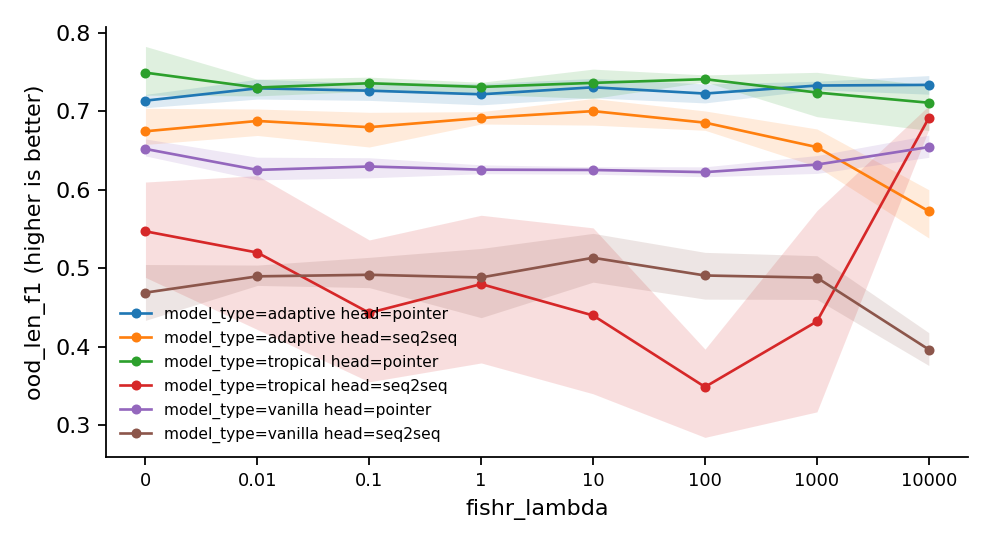
\includegraphics[width=\textwidth]{metric_ood_len_f1.png}
\caption{\texttt{ood\_len\_f1} against \texttt{fishr\_lambda}: the mean over seeds with a 95\% bootstrap CI, one line per combination of the other factors.}
\label{fig:ood_len_f1}
\end{figure}

{\small
\begin{longtable}{lllrlrrr}
\caption{\texttt{ood\_len\_f1} per cell: mean, 95\% bootstrap CI, SD, seeds, diverged runs.}\label{tab:summary-ood_len_f1}\\
\toprule
\texttt{model\_type} & \texttt{head} & \texttt{fishr\_lambda} & mean & 95\% CI & SD & $n$ & div.\\
\midrule
\endhead
adaptive & pointer & 0 & 0.7137 & [0.705, 0.722] & 0.0107 & 5 & 0\\
adaptive & pointer & 0.01 & 0.7294 & [0.716, 0.741] & 0.017 & 5 & 0\\
adaptive & pointer & 0.1 & 0.7264 & [0.714, 0.736] & 0.0147 & 5 & 0\\
adaptive & pointer & 1 & 0.7218 & [0.708, 0.736] & 0.0185 & 5 & 0\\
adaptive & pointer & 10 & 0.7308 & [0.717, 0.742] & 0.016 & 5 & 0\\
adaptive & pointer & 100 & 0.7228 & [0.711, 0.735] & 0.016 & 5 & 0\\
adaptive & pointer & 1000 & 0.733 & [0.728, 0.738] & 0.00699 & 5 & 0\\
adaptive & pointer & 1e+04 & 0.7338 & [0.722, 0.746] & 0.0143 & 5 & 0\\
adaptive & seq2seq & 0 & 0.6747 & [0.658, 0.704] & 0.0326 & 5 & 0\\
adaptive & seq2seq & 0.01 & 0.6878 & [0.669, 0.703] & 0.0212 & 5 & 0\\
adaptive & seq2seq & 0.1 & 0.6799 & [0.655, 0.699] & 0.0283 & 5 & 0\\
adaptive & seq2seq & 1 & 0.6916 & [0.684, 0.7] & 0.00997 & 5 & 0\\
adaptive & seq2seq & 10 & 0.7004 & [0.683, 0.716] & 0.0213 & 5 & 0\\
adaptive & seq2seq & 100 & 0.6857 & [0.676, 0.701] & 0.0164 & 5 & 0\\
adaptive & seq2seq & 1000 & 0.6545 & [0.63, 0.678] & 0.0292 & 5 & 0\\
adaptive & seq2seq & 1e+04 & 0.5728 & [0.539, 0.6] & 0.0412 & 5 & 0\\
tropical & pointer & 0 & 0.7494 & [0.721, 0.783] & 0.0436 & 5 & 0\\
tropical & pointer & 0.01 & 0.7304 & [0.72, 0.741] & 0.0138 & 5 & 0\\
tropical & pointer & 0.1 & 0.7359 & [0.726, 0.744] & 0.0119 & 5 & 0\\
tropical & pointer & 1 & 0.7312 & [0.722, 0.737] & 0.0106 & 5 & 0\\
tropical & pointer & 10 & 0.7364 & [0.716, 0.754] & 0.024 & 5 & 0\\
tropical & pointer & 100 & 0.7411 & [0.738, 0.747] & 0.00605 & 5 & 0\\
tropical & pointer & 1000 & 0.7241 & [0.693, 0.75] & 0.0378 & 5 & 0\\
tropical & pointer & 1e+04 & 0.7111 & [0.676, 0.733] & 0.0393 & 5 & 0\\
tropical & seq2seq & 0 & 0.5472 & [0.488, 0.61] & 0.0809 & 5 & 0\\
tropical & seq2seq & 0.01 & 0.5201 & [0.422, 0.618] & 0.131 & 5 & 0\\
tropical & seq2seq & 0.1 & 0.4432 & [0.355, 0.536] & 0.116 & 5 & 0\\
tropical & seq2seq & 1 & 0.4799 & [0.379, 0.568] & 0.119 & 5 & 0\\
tropical & seq2seq & 10 & 0.4399 & [0.34, 0.552] & 0.137 & 5 & 0\\
tropical & seq2seq & 100 & 0.3488 & [0.285, 0.397] & 0.073 & 5 & 0\\
tropical & seq2seq & 1000 & 0.4323 & [0.317, 0.574] & 0.162 & 5 & 0\\
tropical & seq2seq & 1e+04 & 0.6917 & [0.677, 0.707] & 0.0196 & 5 & 0\\
vanilla & pointer & 0 & 0.6521 & [0.643, 0.665] & 0.0133 & 5 & 0\\
vanilla & pointer & 0.01 & 0.6254 & [0.613, 0.642] & 0.018 & 5 & 0\\
vanilla & pointer & 0.1 & 0.6298 & [0.615, 0.641] & 0.0169 & 5 & 0\\
vanilla & pointer & 1 & 0.6258 & [0.621, 0.632] & 0.00767 & 5 & 0\\
vanilla & pointer & 10 & 0.6254 & [0.62, 0.63] & 0.00612 & 5 & 0\\
vanilla & pointer & 100 & 0.6226 & [0.617, 0.629] & 0.00832 & 5 & 0\\
vanilla & pointer & 1000 & 0.6322 & [0.621, 0.644] & 0.016 & 5 & 0\\
vanilla & pointer & 1e+04 & 0.6546 & [0.641, 0.67] & 0.0174 & 5 & 0\\
vanilla & seq2seq & 0 & 0.469 & [0.434, 0.505] & 0.047 & 5 & 0\\
vanilla & seq2seq & 0.01 & 0.4898 & [0.478, 0.504] & 0.0173 & 5 & 0\\
vanilla & seq2seq & 0.1 & 0.4918 & [0.475, 0.514] & 0.0249 & 5 & 0\\
vanilla & seq2seq & 1 & 0.4884 & [0.437, 0.525] & 0.0532 & 5 & 0\\
vanilla & seq2seq & 10 & 0.5135 & [0.482, 0.545] & 0.0406 & 5 & 0\\
vanilla & seq2seq & 100 & 0.4909 & [0.461, 0.52] & 0.0396 & 5 & 0\\
vanilla & seq2seq & 1000 & 0.4881 & [0.46, 0.516] & 0.0358 & 5 & 0\\
vanilla & seq2seq & 1e+04 & 0.3965 & [0.376, 0.418] & 0.0275 & 5 & 0\\
\bottomrule
\end{longtable}
}

{\small
\begin{longtable}{lllrrrl}
\caption{\texttt{ood\_len\_f1}: each level of \texttt{fishr\_lambda} against its control (0), within each combination of the other factors. parametric: Dunnett vs control.}\label{tab:control-ood_len_f1}\\
\toprule
\texttt{model\_type} & \texttt{head} & \texttt{fishr\_lambda} & difference & 95\% CI & $p$ & \\
\midrule
\endhead
adaptive & pointer & 0.01 & 0.01571 & [-0.00995, 0.0414] & 0.3955 & \\
adaptive & pointer & 0.1 & 0.01271 & [-0.0129, 0.0384] & 0.6103 & \\
adaptive & pointer & 1 & 0.008079 & [-0.0176, 0.0337] & 0.9176 & \\
adaptive & pointer & 10 & 0.01703 & [-0.00864, 0.0427] & 0.3163 & \\
adaptive & pointer & 100 & 0.009039 & [-0.0166, 0.0347] & 0.8691 & \\
adaptive & pointer & 1000 & 0.01926 & [-0.00641, 0.0449] & 0.2082 & \\
adaptive & pointer & 1e+04 & 0.0201 & [-0.00556, 0.0458] & 0.1755 & \\
adaptive & seq2seq & 0.01 & 0.01318 & [-0.0334, 0.0597] & 0.9491 & \\
adaptive & seq2seq & 0.1 & 0.005239 & [-0.0413, 0.0518] & 0.9998 & \\
adaptive & seq2seq & 1 & 0.01694 & [-0.0296, 0.0635] & 0.8520 & \\
adaptive & seq2seq & 10 & 0.02572 & [-0.0209, 0.0723] & 0.5010 & \\
adaptive & seq2seq & 100 & 0.01103 & [-0.0355, 0.0576] & 0.9791 & \\
adaptive & seq2seq & 1000 & -0.02019 & [-0.0668, 0.0264] & 0.7307 & \\
adaptive & seq2seq & 1e+04 & -0.1019 & [-0.148, -0.0553] & $<10^{-4}$ & *\\
tropical & pointer & 0.01 & -0.01897 & [-0.0665, 0.0286] & 0.7937 & \\
tropical & pointer & 0.1 & -0.0135 & [-0.0611, 0.0341] & 0.9484 & \\
tropical & pointer & 1 & -0.01819 & [-0.0657, 0.0294] & 0.8219 & \\
tropical & pointer & 10 & -0.01303 & [-0.0606, 0.0345] & 0.9563 & \\
tropical & pointer & 100 & -0.008305 & [-0.0559, 0.0392] & 0.9962 & \\
tropical & pointer & 1000 & -0.02535 & [-0.0729, 0.0222] & 0.5373 & \\
tropical & pointer & 1e+04 & -0.03835 & [-0.0859, 0.0092] & 0.1552 & \\
tropical & seq2seq & 0.01 & -0.02709 & [-0.224, 0.17] & 0.9991 & \\
tropical & seq2seq & 0.1 & -0.1039 & [-0.301, 0.0932] & 0.5485 & \\
tropical & seq2seq & 1 & -0.06722 & [-0.264, 0.13] & 0.8848 & \\
tropical & seq2seq & 10 & -0.1072 & [-0.304, 0.0899] & 0.5163 & \\
tropical & seq2seq & 100 & -0.1984 & [-0.395, -0.00125] & 0.0480 & *\\
tropical & seq2seq & 1000 & -0.1149 & [-0.312, 0.0822] & 0.4456 & \\
tropical & seq2seq & 1e+04 & 0.1446 & [-0.0525, 0.342] & 0.2265 & \\
vanilla & pointer & 0.01 & -0.02673 & [-0.0508, -0.0027] & 0.0240 & *\\
vanilla & pointer & 0.1 & -0.02235 & [-0.0464, 0.00167] & 0.0765 & \\
vanilla & pointer & 1 & -0.0264 & [-0.0504, -0.00237] & 0.0263 & *\\
vanilla & pointer & 10 & -0.02679 & [-0.0508, -0.00277] & 0.0237 & *\\
vanilla & pointer & 100 & -0.02954 & [-0.0536, -0.00551] & 0.0107 & *\\
vanilla & pointer & 1000 & -0.01994 & [-0.044, 0.00409] & 0.1367 & \\
vanilla & pointer & 1e+04 & 0.002412 & [-0.0216, 0.0264] & 0.9999 & \\
vanilla & seq2seq & 0.01 & 0.02076 & [-0.0446, 0.0862] & 0.9145 & \\
vanilla & seq2seq & 0.1 & 0.02276 & [-0.0426, 0.0882] & 0.8751 & \\
vanilla & seq2seq & 1 & 0.01934 & [-0.0461, 0.0847] & 0.9376 & \\
vanilla & seq2seq & 10 & 0.04445 & [-0.0209, 0.11] & 0.2936 & \\
vanilla & seq2seq & 100 & 0.02185 & [-0.0435, 0.0873] & 0.8939 & \\
vanilla & seq2seq & 1000 & 0.01907 & [-0.0463, 0.0845] & 0.9415 & \\
vanilla & seq2seq & 1e+04 & -0.07253 & [-0.138, -0.00713] & 0.0247 & *\\
\bottomrule
\end{longtable}
}

{\small
\begin{longtable}{llrrrrr}
\caption{\texttt{ood\_len\_f1} against log10 \texttt{fishr\_lambda}: parametric: OLS slope t-test, seed-bootstrap CI, with the Jonckheere--Terpstra ordered-trend $\tau$ and $p$.}\label{tab:trend-ood_len_f1}\\
\toprule
\texttt{model\_type} & \texttt{head} & estimate & 95\% CI & $p$ & JT $\tau$ & JT $p$\\
\midrule
\endhead
adaptive & pointer & $9.724\times10^{-4}$ & [$-8.18\times10^{-4}$, 0.0033] & 0.4352 & 0.124 & 0.3605\\
adaptive & seq2seq & -0.01436 & [-0.0181, -0.0107] & $<10^{-4}$ & -0.467 & 0.0006\\
tropical & pointer & -0.00257 & [-0.00951, 0.00268] & 0.2040 & -0.0629 & 0.6457\\
tropical & seq2seq & 0.01293 & [-0.0101, 0.0285] & 0.3020 & 0.109 & 0.4095\\
vanilla & pointer & 0.003182 & [$-6.68\times10^{-4}$, 0.00793] & 0.0178 & 0.242 & 0.0764\\
vanilla & seq2seq & -0.01017 & [-0.0138, -0.00686] & 0.0103 & -0.265 & 0.0502\\
\bottomrule
\end{longtable}
}

{\small
\begin{longtable}{lrrrl}
\caption{\texttt{ood\_len\_f1}: paired contrasts by seed, Holm-corrected across the cells. parametric: paired t-test by seed, Holm.}\label{tab:paired-ood_len_f1}\\
\toprule
contrast (within) & difference & 95\% CI & $p$ & \\
\midrule
\endhead
\stackcell{model\_type: tropical - vanilla\\\footnotesize head=pointer fishr\_lambda=0 } & 0.09726 & [0.0367, 0.158] & 0.1114 & \\
\stackcell{model\_type: tropical - vanilla\\\footnotesize head=pointer fishr\_lambda=0.01 } & 0.105 & [0.0909, 0.119] & 0.0004 & *\\
\stackcell{model\_type: tropical - vanilla\\\footnotesize head=pointer fishr\_lambda=0.1 } & 0.1061 & [0.0816, 0.131] & 0.0033 & *\\
\stackcell{model\_type: tropical - vanilla\\\footnotesize head=pointer fishr\_lambda=1 } & 0.1055 & [0.0925, 0.118] & 0.0003 & *\\
\stackcell{model\_type: tropical - vanilla\\\footnotesize head=pointer fishr\_lambda=10 } & 0.111 & [0.0837, 0.138] & 0.0039 & *\\
\stackcell{model\_type: tropical - vanilla\\\footnotesize head=pointer fishr\_lambda=100 } & 0.1185 & [0.106, 0.131] & 0.0002 & *\\
\stackcell{model\_type: tropical - vanilla\\\footnotesize head=pointer fishr\_lambda=1000 } & 0.09185 & [0.0345, 0.149] & 0.1114 & \\
\stackcell{model\_type: tropical - vanilla\\\footnotesize head=pointer fishr\_lambda=1e+04 } & 0.05649 & [0.00835, 0.105] & 0.2243 & \\
\stackcell{model\_type: tropical - vanilla\\\footnotesize head=seq2seq fishr\_lambda=0 } & 0.07814 & [-0.0794, 0.236] & 1.0000 & \\
\stackcell{model\_type: tropical - vanilla\\\footnotesize head=seq2seq fishr\_lambda=0.01 } & 0.0303 & [-0.118, 0.179] & 1.0000 & \\
\stackcell{model\_type: tropical - vanilla\\\footnotesize head=seq2seq fishr\_lambda=0.1 } & -0.04853 & [-0.216, 0.119] & 1.0000 & \\
\stackcell{model\_type: tropical - vanilla\\\footnotesize head=seq2seq fishr\_lambda=1 } & -0.008412 & [-0.21, 0.193] & 1.0000 & \\
\stackcell{model\_type: tropical - vanilla\\\footnotesize head=seq2seq fishr\_lambda=10 } & -0.07355 & [-0.288, 0.141] & 1.0000 & \\
\stackcell{model\_type: tropical - vanilla\\\footnotesize head=seq2seq fishr\_lambda=100 } & -0.1421 & [-0.259, -0.025] & 0.2243 & \\
\stackcell{model\_type: tropical - vanilla\\\footnotesize head=seq2seq fishr\_lambda=1000 } & -0.05579 & [-0.27, 0.158] & 1.0000 & \\
\stackcell{model\_type: tropical - vanilla\\\footnotesize head=seq2seq fishr\_lambda=1e+04 } & 0.2953 & [0.258, 0.333] & 0.0004 & *\\
\stackcell{model\_type: adaptive - vanilla\\\footnotesize head=pointer fishr\_lambda=0 } & 0.06158 & [0.0327, 0.0904] & 0.0057 & *\\
\stackcell{model\_type: adaptive - vanilla\\\footnotesize head=pointer fishr\_lambda=0.01 } & 0.104 & [0.0907, 0.117] & 0.0004 & *\\
\stackcell{model\_type: adaptive - vanilla\\\footnotesize head=pointer fishr\_lambda=0.1 } & 0.09665 & [0.0869, 0.106] & 0.0002 & *\\
\stackcell{model\_type: adaptive - vanilla\\\footnotesize head=pointer fishr\_lambda=1 } & 0.09605 & [0.0758, 0.116] & 0.0024 & *\\
\stackcell{model\_type: adaptive - vanilla\\\footnotesize head=pointer fishr\_lambda=10 } & 0.1054 & [0.0833, 0.127] & 0.0024 & *\\
\stackcell{model\_type: adaptive - vanilla\\\footnotesize head=pointer fishr\_lambda=100 } & 0.1002 & [0.0711, 0.129] & 0.0042 & *\\
\stackcell{model\_type: adaptive - vanilla\\\footnotesize head=pointer fishr\_lambda=1000 } & 0.1008 & [0.0763, 0.125] & 0.0034 & *\\
\stackcell{model\_type: adaptive - vanilla\\\footnotesize head=pointer fishr\_lambda=1e+04 } & 0.07927 & [0.0512, 0.107] & 0.0057 & *\\
\stackcell{model\_type: adaptive - vanilla\\\footnotesize head=seq2seq fishr\_lambda=0 } & 0.2056 & [0.12, 0.292] & 0.0057 & *\\
\stackcell{model\_type: adaptive - vanilla\\\footnotesize head=seq2seq fishr\_lambda=0.01 } & 0.1981 & [0.178, 0.219] & 0.0002 & *\\
\stackcell{model\_type: adaptive - vanilla\\\footnotesize head=seq2seq fishr\_lambda=0.1 } & 0.1881 & [0.147, 0.23] & 0.0025 & *\\
\stackcell{model\_type: adaptive - vanilla\\\footnotesize head=seq2seq fishr\_lambda=1 } & 0.2032 & [0.129, 0.278] & 0.0057 & *\\
\stackcell{model\_type: adaptive - vanilla\\\footnotesize head=seq2seq fishr\_lambda=10 } & 0.1869 & [0.133, 0.241] & 0.0042 & *\\
\stackcell{model\_type: adaptive - vanilla\\\footnotesize head=seq2seq fishr\_lambda=100 } & 0.1948 & [0.145, 0.244] & 0.0036 & *\\
\stackcell{model\_type: adaptive - vanilla\\\footnotesize head=seq2seq fishr\_lambda=1000 } & 0.1664 & [0.121, 0.212] & 0.0042 & *\\
\stackcell{model\_type: adaptive - vanilla\\\footnotesize head=seq2seq fishr\_lambda=1e+04 } & 0.1763 & [0.128, 0.225] & 0.0042 & *\\
\stackcell{head: pointer - seq2seq\\\footnotesize model\_type=adaptive fishr\_lambda=0 } & 0.03906 & [0.00426, 0.0739] & 0.1850 & \\
\stackcell{head: pointer - seq2seq\\\footnotesize model\_type=adaptive fishr\_lambda=0.01 } & 0.0416 & [$-8.78\times10^{-4}$, 0.0841] & 0.2063 & \\
\stackcell{head: pointer - seq2seq\\\footnotesize model\_type=adaptive fishr\_lambda=0.1 } & 0.04654 & [$-5.09\times10^{-4}$, 0.0936] & 0.2063 & \\
\stackcell{head: pointer - seq2seq\\\footnotesize model\_type=adaptive fishr\_lambda=1 } & 0.03021 & [0.00535, 0.0551] & 0.1850 & \\
\stackcell{head: pointer - seq2seq\\\footnotesize model\_type=adaptive fishr\_lambda=10 } & 0.03037 & [-0.0116, 0.0723] & 0.2297 & \\
\stackcell{head: pointer - seq2seq\\\footnotesize model\_type=adaptive fishr\_lambda=100 } & 0.03708 & [0.00834, 0.0658] & 0.1850 & \\
\stackcell{head: pointer - seq2seq\\\footnotesize model\_type=adaptive fishr\_lambda=1000 } & 0.07851 & [0.0364, 0.121] & 0.0859 & \\
\stackcell{head: pointer - seq2seq\\\footnotesize model\_type=adaptive fishr\_lambda=1e+04 } & 0.1611 & [0.111, 0.211] & 0.0160 & *\\
\stackcell{head: pointer - seq2seq\\\footnotesize model\_type=tropical fishr\_lambda=0 } & 0.2022 & [0.0602, 0.344] & 0.1511 & \\
\stackcell{head: pointer - seq2seq\\\footnotesize model\_type=tropical fishr\_lambda=0.01 } & 0.2104 & [0.0445, 0.376] & 0.1850 & \\
\stackcell{head: pointer - seq2seq\\\footnotesize model\_type=tropical fishr\_lambda=0.1 } & 0.2927 & [0.156, 0.429] & 0.0563 & \\
\stackcell{head: pointer - seq2seq\\\footnotesize model\_type=tropical fishr\_lambda=1 } & 0.2513 & [0.113, 0.39] & 0.0859 & \\
\stackcell{head: pointer - seq2seq\\\footnotesize model\_type=tropical fishr\_lambda=10 } & 0.2965 & [0.136, 0.457] & 0.0859 & \\
\stackcell{head: pointer - seq2seq\\\footnotesize model\_type=tropical fishr\_lambda=100 } & 0.3923 & [0.304, 0.48] & 0.0057 & *\\
\stackcell{head: pointer - seq2seq\\\footnotesize model\_type=tropical fishr\_lambda=1000 } & 0.2918 & [0.117, 0.467] & 0.0981 & \\
\stackcell{head: pointer - seq2seq\\\footnotesize model\_type=tropical fishr\_lambda=1e+04 } & 0.01931 & [-0.0322, 0.0709] & 0.3570 & \\
\stackcell{head: pointer - seq2seq\\\footnotesize model\_type=vanilla fishr\_lambda=0 } & 0.1831 & [0.13, 0.236] & 0.0132 & *\\
\stackcell{head: pointer - seq2seq\\\footnotesize model\_type=vanilla fishr\_lambda=0.01 } & 0.1356 & [0.0974, 0.174] & 0.0126 & *\\
\stackcell{head: pointer - seq2seq\\\footnotesize model\_type=vanilla fishr\_lambda=0.1 } & 0.138 & [0.103, 0.173] & 0.0087 & *\\
\stackcell{head: pointer - seq2seq\\\footnotesize model\_type=vanilla fishr\_lambda=1 } & 0.1374 & [0.077, 0.198] & 0.0513 & \\
\stackcell{head: pointer - seq2seq\\\footnotesize model\_type=vanilla fishr\_lambda=10 } & 0.1119 & [0.0611, 0.163] & 0.0544 & \\
\stackcell{head: pointer - seq2seq\\\footnotesize model\_type=vanilla fishr\_lambda=100 } & 0.1317 & [0.0771, 0.186] & 0.0440 & *\\
\stackcell{head: pointer - seq2seq\\\footnotesize model\_type=vanilla fishr\_lambda=1000 } & 0.1441 & [0.101, 0.187] & 0.0141 & *\\
\stackcell{head: pointer - seq2seq\\\footnotesize model\_type=vanilla fishr\_lambda=1e+04 } & 0.2581 & [0.221, 0.296] & 0.0011 & *\\
\bottomrule
\end{longtable}
}

\clearpage
\appendix
\section{Other metrics}
\subsection{\texttt{ood\_len\_exact}}
\begin{figure}[tbp]
\centering
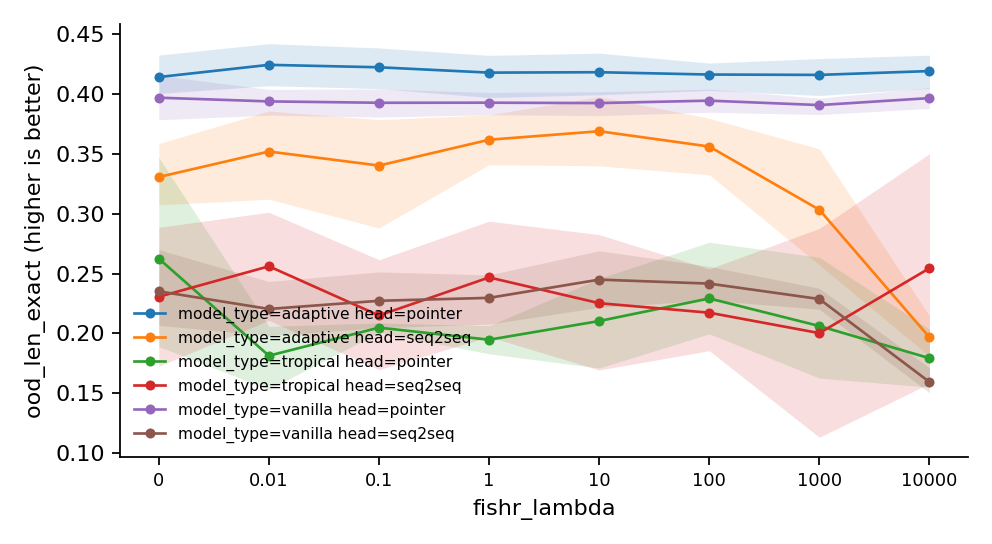
\includegraphics[width=\textwidth]{metric_ood_len_exact.png}
\caption{\texttt{ood\_len\_exact} against \texttt{fishr\_lambda}: the mean over seeds with a 95\% bootstrap CI, one line per combination of the other factors.}
\label{fig:ood_len_exact}
\end{figure}

{\small
\begin{longtable}{lllrlrrr}
\caption{\texttt{ood\_len\_exact} per cell: mean, 95\% bootstrap CI, SD, seeds, diverged runs.}\label{tab:summary-ood_len_exact}\\
\toprule
\texttt{model\_type} & \texttt{head} & \texttt{fishr\_lambda} & mean & 95\% CI & SD & $n$ & div.\\
\midrule
\endhead
adaptive & pointer & 0 & 0.4144 & [0.401, 0.433] & 0.0204 & 5 & 0\\
adaptive & pointer & 0.01 & 0.4246 & [0.407, 0.442] & 0.0213 & 5 & 0\\
adaptive & pointer & 0.1 & 0.4225 & [0.405, 0.439] & 0.0221 & 5 & 0\\
adaptive & pointer & 1 & 0.4181 & [0.397, 0.432] & 0.022 & 5 & 0\\
adaptive & pointer & 10 & 0.4184 & [0.4, 0.434] & 0.0205 & 5 & 0\\
adaptive & pointer & 100 & 0.4165 & [0.403, 0.426] & 0.0152 & 5 & 0\\
adaptive & pointer & 1000 & 0.4162 & [0.399, 0.43] & 0.02 & 5 & 0\\
adaptive & pointer & 1e+04 & 0.4194 & [0.405, 0.433] & 0.0188 & 5 & 0\\
adaptive & seq2seq & 0 & 0.3308 & [0.307, 0.359] & 0.0346 & 5 & 0\\
adaptive & seq2seq & 0.01 & 0.3521 & [0.312, 0.386] & 0.047 & 5 & 0\\
adaptive & seq2seq & 0.1 & 0.3404 & [0.288, 0.379] & 0.0575 & 5 & 0\\
adaptive & seq2seq & 1 & 0.3619 & [0.341, 0.383] & 0.0266 & 5 & 0\\
adaptive & seq2seq & 10 & 0.3691 & [0.34, 0.398] & 0.04 & 5 & 0\\
adaptive & seq2seq & 100 & 0.3563 & [0.333, 0.38] & 0.031 & 5 & 0\\
adaptive & seq2seq & 1000 & 0.3034 & [0.257, 0.354] & 0.0599 & 5 & 0\\
adaptive & seq2seq & 1e+04 & 0.1967 & [0.181, 0.215] & 0.0203 & 5 & 0\\
tropical & pointer & 0 & 0.2626 & [0.189, 0.347] & 0.106 & 5 & 0\\
tropical & pointer & 0.01 & 0.1814 & [0.153, 0.206] & 0.0345 & 5 & 0\\
tropical & pointer & 0.1 & 0.2048 & [0.201, 0.209] & 0.00521 & 5 & 0\\
tropical & pointer & 1 & 0.1947 & [0.183, 0.207] & 0.0156 & 5 & 0\\
tropical & pointer & 10 & 0.2104 & [0.171, 0.246] & 0.0453 & 5 & 0\\
tropical & pointer & 100 & 0.2293 & [0.2, 0.276] & 0.0532 & 5 & 0\\
tropical & pointer & 1000 & 0.2062 & [0.163, 0.264] & 0.067 & 5 & 0\\
tropical & pointer & 1e+04 & 0.1793 & [0.155, 0.204] & 0.0335 & 5 & 0\\
tropical & seq2seq & 0 & 0.2307 & [0.173, 0.289] & 0.0735 & 5 & 0\\
tropical & seq2seq & 0.01 & 0.2561 & [0.211, 0.301] & 0.0609 & 5 & 0\\
tropical & seq2seq & 0.1 & 0.215 & [0.17, 0.262] & 0.0618 & 5 & 0\\
tropical & seq2seq & 1 & 0.2468 & [0.197, 0.294] & 0.0614 & 5 & 0\\
tropical & seq2seq & 10 & 0.2253 & [0.169, 0.283] & 0.0731 & 5 & 0\\
tropical & seq2seq & 100 & 0.2173 & [0.186, 0.254] & 0.0421 & 5 & 0\\
tropical & seq2seq & 1000 & 0.2003 & [0.113, 0.288] & 0.111 & 5 & 0\\
tropical & seq2seq & 1e+04 & 0.2545 & [0.158, 0.35] & 0.128 & 5 & 0\\
vanilla & pointer & 0 & 0.3971 & [0.379, 0.416] & 0.0246 & 5 & 0\\
vanilla & pointer & 0.01 & 0.394 & [0.383, 0.404] & 0.0136 & 5 & 0\\
vanilla & pointer & 0.1 & 0.3929 & [0.381, 0.404] & 0.015 & 5 & 0\\
vanilla & pointer & 1 & 0.3929 & [0.383, 0.401] & 0.0118 & 5 & 0\\
vanilla & pointer & 10 & 0.3926 & [0.382, 0.402] & 0.0133 & 5 & 0\\
vanilla & pointer & 100 & 0.3946 & [0.385, 0.404] & 0.0124 & 5 & 0\\
vanilla & pointer & 1000 & 0.3909 & [0.383, 0.397] & 0.00897 & 5 & 0\\
vanilla & pointer & 1e+04 & 0.3968 & [0.388, 0.405] & 0.0111 & 5 & 0\\
vanilla & seq2seq & 0 & 0.2352 & [0.207, 0.27] & 0.0397 & 5 & 0\\
vanilla & seq2seq & 0.01 & 0.2205 & [0.198, 0.243] & 0.0292 & 5 & 0\\
vanilla & seq2seq & 0.1 & 0.2273 & [0.205, 0.251] & 0.0303 & 5 & 0\\
vanilla & seq2seq & 1 & 0.2297 & [0.208, 0.249] & 0.0248 & 5 & 0\\
vanilla & seq2seq & 10 & 0.245 & [0.222, 0.269] & 0.0308 & 5 & 0\\
vanilla & seq2seq & 100 & 0.2417 & [0.228, 0.256] & 0.0185 & 5 & 0\\
vanilla & seq2seq & 1000 & 0.2288 & [0.22, 0.238] & 0.0116 & 5 & 0\\
vanilla & seq2seq & 1e+04 & 0.1594 & [0.15, 0.171] & 0.0134 & 5 & 0\\
\bottomrule
\end{longtable}
}

{\small
\begin{longtable}{lllrrrl}
\caption{\texttt{ood\_len\_exact}: each level of \texttt{fishr\_lambda} against its control (0), within each combination of the other factors. parametric: Dunnett vs control.}\label{tab:control-ood_len_exact}\\
\toprule
\texttt{model\_type} & \texttt{head} & \texttt{fishr\_lambda} & difference & 95\% CI & $p$ & \\
\midrule
\endhead
adaptive & pointer & 0.01 & 0.0102 & [-0.025, 0.0454] & 0.9430 & \\
adaptive & pointer & 0.1 & 0.008167 & [-0.027, 0.0434] & 0.9812 & \\
adaptive & pointer & 1 & 0.0037 & [-0.0315, 0.0389] & 0.9998 & \\
adaptive & pointer & 10 & 0.004033 & [-0.0312, 0.0392] & 0.9997 & \\
adaptive & pointer & 100 & 0.0021 & [-0.0331, 0.0373] & 1.0000 & \\
adaptive & pointer & 1000 & 0.0018 & [-0.0334, 0.037] & 1.0000 & \\
adaptive & pointer & 1e+04 & 0.005 & [-0.0302, 0.0402] & 0.9989 & \\
adaptive & seq2seq & 0.01 & 0.0213 & [-0.0517, 0.0943] & 0.9413 & \\
adaptive & seq2seq & 0.1 & 0.009567 & [-0.0635, 0.0826] & 0.9994 & \\
adaptive & seq2seq & 1 & 0.03113 & [-0.0419, 0.104] & 0.7440 & \\
adaptive & seq2seq & 10 & 0.03827 & [-0.0348, 0.111] & 0.5544 & \\
adaptive & seq2seq & 100 & 0.02547 & [-0.0476, 0.0985] & 0.8740 & \\
adaptive & seq2seq & 1000 & -0.0274 & [-0.1, 0.0456] & 0.8337 & \\
adaptive & seq2seq & 1e+04 & -0.1341 & [-0.207, -0.061] & 0.0001 & *\\
tropical & pointer & 0.01 & -0.0812 & [-0.175, 0.0127] & 0.1128 & \\
tropical & pointer & 0.1 & -0.05773 & [-0.152, 0.0362] & 0.3916 & \\
tropical & pointer & 1 & -0.06783 & [-0.162, 0.0261] & 0.2399 & \\
tropical & pointer & 10 & -0.0522 & [-0.146, 0.0417] & 0.4947 & \\
tropical & pointer & 100 & -0.0333 & [-0.127, 0.0606] & 0.8658 & \\
tropical & pointer & 1000 & -0.05637 & [-0.15, 0.0376] & 0.4159 & \\
tropical & pointer & 1e+04 & -0.08327 & [-0.177, 0.0107] & 0.0994 & \\
tropical & seq2seq & 0.01 & 0.02547 & [-0.116, 0.167] & 0.9956 & \\
tropical & seq2seq & 0.1 & -0.01567 & [-0.157, 0.126] & 0.9998 & \\
tropical & seq2seq & 1 & 0.01617 & [-0.126, 0.158] & 0.9997 & \\
tropical & seq2seq & 10 & -0.005367 & [-0.147, 0.136] & 1.0000 & \\
tropical & seq2seq & 100 & -0.01333 & [-0.155, 0.128] & 0.9999 & \\
tropical & seq2seq & 1000 & -0.0304 & [-0.172, 0.111] & 0.9877 & \\
tropical & seq2seq & 1e+04 & 0.02387 & [-0.118, 0.166] & 0.9970 & \\
vanilla & pointer & 0.01 & -0.0031 & [-0.0285, 0.0223] & 0.9996 & \\
vanilla & pointer & 0.1 & -0.004233 & [-0.0296, 0.0211] & 0.9971 & \\
vanilla & pointer & 1 & -0.004167 & [-0.0295, 0.0212] & 0.9974 & \\
vanilla & pointer & 10 & -0.0045 & [-0.0299, 0.0209] & 0.9959 & \\
vanilla & pointer & 100 & -0.002467 & [-0.0278, 0.0229] & 0.9999 & \\
vanilla & pointer & 1000 & -0.006167 & [-0.0315, 0.0192] & 0.9760 & \\
vanilla & pointer & 1e+04 & $-3.333\times10^{-4}$ & [-0.0257, 0.025] & 1.0000 & \\
vanilla & seq2seq & 0.01 & -0.01473 & [-0.0608, 0.0313] & 0.9117 & \\
vanilla & seq2seq & 0.1 & -0.0079 & [-0.054, 0.0382] & 0.9966 & \\
vanilla & seq2seq & 1 & -0.005467 & [-0.0515, 0.0406] & 0.9997 & \\
vanilla & seq2seq & 10 & 0.0098 & [-0.0363, 0.0559] & 0.9883 & \\
vanilla & seq2seq & 100 & 0.006467 & [-0.0396, 0.0525] & 0.9990 & \\
vanilla & seq2seq & 1000 & -0.006433 & [-0.0525, 0.0396] & 0.9991 & \\
vanilla & seq2seq & 1e+04 & -0.0758 & [-0.122, -0.0297] & 0.0005 & *\\
\bottomrule
\end{longtable}
}

{\small
\begin{longtable}{llrrrrr}
\caption{\texttt{ood\_len\_exact} against log10 \texttt{fishr\_lambda}: parametric: OLS slope t-test, seed-bootstrap CI, with the Jonckheere--Terpstra ordered-trend $\tau$ and $p$.}\label{tab:trend-ood_len_exact}\\
\toprule
\texttt{model\_type} & \texttt{head} & estimate & 95\% CI & $p$ & JT $\tau$ & JT $p$\\
\midrule
\endhead
adaptive & pointer & -0.001069 & [-0.00185, $-4.86\times10^{-4}$] & 0.5018 & -0.103 & 0.4449\\
adaptive & seq2seq & -0.01949 & [-0.0266, -0.0139] & 0.0003 & -0.379 & 0.0036\\
tropical & pointer & 0.00111 & [-0.00458, 0.0101] & 0.7536 & 0.0438 & 0.7536\\
tropical & seq2seq & -0.002277 & [-0.0163, 0.012] & 0.7331 & -0.0667 & 0.6173\\
vanilla & pointer & $2.190\times10^{-4}$ & [-0.00104, 0.00143] & 0.8242 & 0 & 1.0000\\
vanilla & seq2seq & -0.006012 & [-0.00922, -0.00287] & 0.0380 & -0.21 & 0.1114\\
\bottomrule
\end{longtable}
}

{\small
\begin{longtable}{lrrrl}
\caption{\texttt{ood\_len\_exact}: paired contrasts by seed, Holm-corrected across the cells. parametric: paired t-test by seed, Holm.}\label{tab:paired-ood_len_exact}\\
\toprule
contrast (within) & difference & 95\% CI & $p$ & \\
\midrule
\endhead
\stackcell{model\_type: tropical - vanilla\\\footnotesize head=pointer fishr\_lambda=0 } & -0.1345 & [-0.253, -0.0156] & 0.3133 & \\
\stackcell{model\_type: tropical - vanilla\\\footnotesize head=pointer fishr\_lambda=0.01 } & -0.2126 & [-0.269, -0.156] & 0.0062 & *\\
\stackcell{model\_type: tropical - vanilla\\\footnotesize head=pointer fishr\_lambda=0.1 } & -0.188 & [-0.204, -0.172] & $<10^{-4}$ & *\\
\stackcell{model\_type: tropical - vanilla\\\footnotesize head=pointer fishr\_lambda=1 } & -0.1982 & [-0.225, -0.171] & 0.0005 & *\\
\stackcell{model\_type: tropical - vanilla\\\footnotesize head=pointer fishr\_lambda=10 } & -0.1822 & [-0.242, -0.122] & 0.0128 & *\\
\stackcell{model\_type: tropical - vanilla\\\footnotesize head=pointer fishr\_lambda=100 } & -0.1654 & [-0.225, -0.106] & 0.0164 & *\\
\stackcell{model\_type: tropical - vanilla\\\footnotesize head=pointer fishr\_lambda=1000 } & -0.1847 & [-0.27, -0.0999] & 0.0378 & *\\
\stackcell{model\_type: tropical - vanilla\\\footnotesize head=pointer fishr\_lambda=1e+04 } & -0.2175 & [-0.264, -0.171] & 0.0028 & *\\
\stackcell{model\_type: tropical - vanilla\\\footnotesize head=seq2seq fishr\_lambda=0 } & -0.004533 & [-0.132, 0.123] & 1.0000 & \\
\stackcell{model\_type: tropical - vanilla\\\footnotesize head=seq2seq fishr\_lambda=0.01 } & 0.03567 & [-0.0516, 0.123] & 1.0000 & \\
\stackcell{model\_type: tropical - vanilla\\\footnotesize head=seq2seq fishr\_lambda=0.1 } & -0.0123 & [-0.125, 0.1] & 1.0000 & \\
\stackcell{model\_type: tropical - vanilla\\\footnotesize head=seq2seq fishr\_lambda=1 } & 0.0171 & [-0.0621, 0.0963] & 1.0000 & \\
\stackcell{model\_type: tropical - vanilla\\\footnotesize head=seq2seq fishr\_lambda=10 } & -0.0197 & [-0.145, 0.106] & 1.0000 & \\
\stackcell{model\_type: tropical - vanilla\\\footnotesize head=seq2seq fishr\_lambda=100 } & -0.02433 & [-0.0947, 0.0461] & 1.0000 & \\
\stackcell{model\_type: tropical - vanilla\\\footnotesize head=seq2seq fishr\_lambda=1000 } & -0.0285 & [-0.18, 0.123] & 1.0000 & \\
\stackcell{model\_type: tropical - vanilla\\\footnotesize head=seq2seq fishr\_lambda=1e+04 } & 0.09513 & [-0.0613, 0.252] & 1.0000 & \\
\stackcell{model\_type: adaptive - vanilla\\\footnotesize head=pointer fishr\_lambda=0 } & 0.01727 & [0.0015, 0.033] & 0.2685 & \\
\stackcell{model\_type: adaptive - vanilla\\\footnotesize head=pointer fishr\_lambda=0.01 } & 0.03057 & [-0.00445, 0.0656] & 0.3632 & \\
\stackcell{model\_type: adaptive - vanilla\\\footnotesize head=pointer fishr\_lambda=0.1 } & 0.02967 & [-0.00667, 0.066] & 0.3632 & \\
\stackcell{model\_type: adaptive - vanilla\\\footnotesize head=pointer fishr\_lambda=1 } & 0.02513 & [-0.0076, 0.0579] & 0.3632 & \\
\stackcell{model\_type: adaptive - vanilla\\\footnotesize head=pointer fishr\_lambda=10 } & 0.0258 & [-0.0047, 0.0563] & 0.3632 & \\
\stackcell{model\_type: adaptive - vanilla\\\footnotesize head=pointer fishr\_lambda=100 } & 0.02183 & [-0.00348, 0.0471] & 0.3632 & \\
\stackcell{model\_type: adaptive - vanilla\\\footnotesize head=pointer fishr\_lambda=1000 } & 0.02523 & [-0.00179, 0.0523] & 0.3632 & \\
\stackcell{model\_type: adaptive - vanilla\\\footnotesize head=pointer fishr\_lambda=1e+04 } & 0.0226 & [0.00418, 0.041] & 0.2437 & \\
\stackcell{model\_type: adaptive - vanilla\\\footnotesize head=seq2seq fishr\_lambda=0 } & 0.0956 & [0.0203, 0.171] & 0.2437 & \\
\stackcell{model\_type: adaptive - vanilla\\\footnotesize head=seq2seq fishr\_lambda=0.01 } & 0.1316 & [0.0876, 0.176] & 0.0156 & *\\
\stackcell{model\_type: adaptive - vanilla\\\footnotesize head=seq2seq fishr\_lambda=0.1 } & 0.1131 & [0.0569, 0.169] & 0.0602 & \\
\stackcell{model\_type: adaptive - vanilla\\\footnotesize head=seq2seq fishr\_lambda=1 } & 0.1322 & [0.0883, 0.176] & 0.0156 & *\\
\stackcell{model\_type: adaptive - vanilla\\\footnotesize head=seq2seq fishr\_lambda=10 } & 0.1241 & [0.0842, 0.164] & 0.0148 & *\\
\stackcell{model\_type: adaptive - vanilla\\\footnotesize head=seq2seq fishr\_lambda=100 } & 0.1146 & [0.0916, 0.138] & 0.0025 & *\\
\stackcell{model\_type: adaptive - vanilla\\\footnotesize head=seq2seq fishr\_lambda=1000 } & 0.07463 & [0.0139, 0.135] & 0.2437 & \\
\stackcell{model\_type: adaptive - vanilla\\\footnotesize head=seq2seq fishr\_lambda=1e+04 } & 0.03733 & [0.0118, 0.0629] & 0.1697 & \\
\stackcell{head: pointer - seq2seq\\\footnotesize model\_type=adaptive fishr\_lambda=0 } & 0.08357 & [0.0312, 0.136] & 0.1716 & \\
\stackcell{head: pointer - seq2seq\\\footnotesize model\_type=adaptive fishr\_lambda=0.01 } & 0.07247 & [-0.00192, 0.147] & 0.5114 & \\
\stackcell{head: pointer - seq2seq\\\footnotesize model\_type=adaptive fishr\_lambda=0.1 } & 0.08217 & [$-6.55\times10^{-4}$, 0.165] & 0.5114 & \\
\stackcell{head: pointer - seq2seq\\\footnotesize model\_type=adaptive fishr\_lambda=1 } & 0.05613 & [0.00192, 0.11] & 0.4977 & \\
\stackcell{head: pointer - seq2seq\\\footnotesize model\_type=adaptive fishr\_lambda=10 } & 0.04933 & [-0.0171, 0.116] & 0.8645 & \\
\stackcell{head: pointer - seq2seq\\\footnotesize model\_type=adaptive fishr\_lambda=100 } & 0.0602 & [0.00989, 0.111] & 0.3811 & \\
\stackcell{head: pointer - seq2seq\\\footnotesize model\_type=adaptive fishr\_lambda=1000 } & 0.1128 & [0.0171, 0.208] & 0.3811 & \\
\stackcell{head: pointer - seq2seq\\\footnotesize model\_type=adaptive fishr\_lambda=1e+04 } & 0.2226 & [0.197, 0.249] & 0.0004 & *\\
\stackcell{head: pointer - seq2seq\\\footnotesize model\_type=tropical fishr\_lambda=0 } & 0.0319 & [-0.146, 0.21] & 1.0000 & \\
\stackcell{head: pointer - seq2seq\\\footnotesize model\_type=tropical fishr\_lambda=0.01 } & -0.07477 & [-0.135, -0.0141] & 0.3743 & \\
\stackcell{head: pointer - seq2seq\\\footnotesize model\_type=tropical fishr\_lambda=0.1 } & -0.01017 & [-0.0913, 0.0709] & 1.0000 & \\
\stackcell{head: pointer - seq2seq\\\footnotesize model\_type=tropical fishr\_lambda=1 } & -0.0521 & [-0.129, 0.0251] & 0.9388 & \\
\stackcell{head: pointer - seq2seq\\\footnotesize model\_type=tropical fishr\_lambda=10 } & -0.01493 & [-0.125, 0.0955] & 1.0000 & \\
\stackcell{head: pointer - seq2seq\\\footnotesize model\_type=tropical fishr\_lambda=100 } & 0.01193 & [-0.0396, 0.0634] & 1.0000 & \\
\stackcell{head: pointer - seq2seq\\\footnotesize model\_type=tropical fishr\_lambda=1000 } & 0.005933 & [-0.0929, 0.105] & 1.0000 & \\
\stackcell{head: pointer - seq2seq\\\footnotesize model\_type=tropical fishr\_lambda=1e+04 } & -0.07523 & [-0.23, 0.0793] & 1.0000 & \\
\stackcell{head: pointer - seq2seq\\\footnotesize model\_type=vanilla fishr\_lambda=0 } & 0.1619 & [0.116, 0.208] & 0.0100 & *\\
\stackcell{head: pointer - seq2seq\\\footnotesize model\_type=vanilla fishr\_lambda=0.01 } & 0.1735 & [0.143, 0.204] & 0.0019 & *\\
\stackcell{head: pointer - seq2seq\\\footnotesize model\_type=vanilla fishr\_lambda=0.1 } & 0.1656 & [0.131, 0.2] & 0.0034 & *\\
\stackcell{head: pointer - seq2seq\\\footnotesize model\_type=vanilla fishr\_lambda=1 } & 0.1632 & [0.128, 0.199] & 0.0038 & *\\
\stackcell{head: pointer - seq2seq\\\footnotesize model\_type=vanilla fishr\_lambda=10 } & 0.1476 & [0.116, 0.18] & 0.0038 & *\\
\stackcell{head: pointer - seq2seq\\\footnotesize model\_type=vanilla fishr\_lambda=100 } & 0.153 & [0.129, 0.177] & 0.0013 & *\\
\stackcell{head: pointer - seq2seq\\\footnotesize model\_type=vanilla fishr\_lambda=1000 } & 0.1622 & [0.148, 0.176] & 0.0001 & *\\
\stackcell{head: pointer - seq2seq\\\footnotesize model\_type=vanilla fishr\_lambda=1e+04 } & 0.2374 & [0.211, 0.263] & 0.0003 & *\\
\bottomrule
\end{longtable}
}

\subsection{\texttt{ood\_val\_f1}}
\begin{figure}[tbp]
\centering
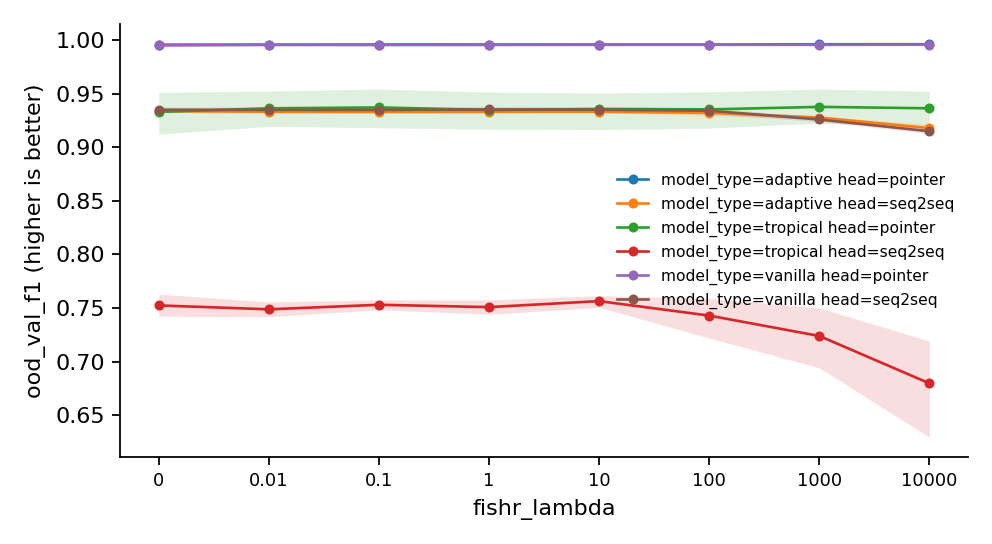
\includegraphics[width=\textwidth]{metric_ood_val_f1.png}
\caption{\texttt{ood\_val\_f1} against \texttt{fishr\_lambda}: the mean over seeds with a 95\% bootstrap CI, one line per combination of the other factors.}
\label{fig:ood_val_f1}
\end{figure}

{\small
\begin{longtable}{lllrlrrr}
\caption{\texttt{ood\_val\_f1} per cell: mean, 95\% bootstrap CI, SD, seeds, diverged runs.}\label{tab:summary-ood_val_f1}\\
\toprule
\texttt{model\_type} & \texttt{head} & \texttt{fishr\_lambda} & mean & 95\% CI & SD & $n$ & div.\\
\midrule
\endhead
adaptive & pointer & 0 & 0.9957 & [0.995, 0.997] & 0.00113 & 5 & 0\\
adaptive & pointer & 0.01 & 0.9957 & [0.995, 0.996] & $6.68\times10^{-4}$ & 5 & 0\\
adaptive & pointer & 0.1 & 0.9958 & [0.995, 0.996] & $5.39\times10^{-4}$ & 5 & 0\\
adaptive & pointer & 1 & 0.9958 & [0.995, 0.996] & $4.69\times10^{-4}$ & 5 & 0\\
adaptive & pointer & 10 & 0.9957 & [0.995, 0.996] & $5.12\times10^{-4}$ & 5 & 0\\
adaptive & pointer & 100 & 0.9957 & [0.995, 0.996] & $5.03\times10^{-4}$ & 5 & 0\\
adaptive & pointer & 1000 & 0.996 & [0.996, 0.996] & $4.11\times10^{-4}$ & 5 & 0\\
adaptive & pointer & 1e+04 & 0.996 & [0.996, 0.996] & $2.87\times10^{-4}$ & 5 & 0\\
adaptive & seq2seq & 0 & 0.9336 & [0.933, 0.934] & 0.0012 & 5 & 0\\
adaptive & seq2seq & 0.01 & 0.9331 & [0.932, 0.934] & 0.00161 & 5 & 0\\
adaptive & seq2seq & 0.1 & 0.9329 & [0.932, 0.934] & 0.00147 & 5 & 0\\
adaptive & seq2seq & 1 & 0.9331 & [0.932, 0.934] & 0.00158 & 5 & 0\\
adaptive & seq2seq & 10 & 0.9331 & [0.932, 0.934] & 0.0013 & 5 & 0\\
adaptive & seq2seq & 100 & 0.9321 & [0.93, 0.935] & 0.00316 & 5 & 0\\
adaptive & seq2seq & 1000 & 0.9277 & [0.926, 0.929] & 0.00218 & 5 & 0\\
adaptive & seq2seq & 1e+04 & 0.9178 & [0.915, 0.921] & 0.00403 & 5 & 0\\
tropical & pointer & 0 & 0.9329 & [0.912, 0.951] & 0.0262 & 5 & 0\\
tropical & pointer & 0.01 & 0.9362 & [0.919, 0.952] & 0.0226 & 5 & 0\\
tropical & pointer & 0.1 & 0.9371 & [0.918, 0.954] & 0.0239 & 5 & 0\\
tropical & pointer & 1 & 0.9347 & [0.917, 0.951] & 0.0218 & 5 & 0\\
tropical & pointer & 10 & 0.9356 & [0.916, 0.951] & 0.0217 & 5 & 0\\
tropical & pointer & 100 & 0.9352 & [0.918, 0.952] & 0.0223 & 5 & 0\\
tropical & pointer & 1000 & 0.9376 & [0.922, 0.954] & 0.0208 & 5 & 0\\
tropical & pointer & 1e+04 & 0.9363 & [0.919, 0.952] & 0.0213 & 5 & 0\\
tropical & seq2seq & 0 & 0.7523 & [0.742, 0.763] & 0.0138 & 5 & 0\\
tropical & seq2seq & 0.01 & 0.7487 & [0.742, 0.756] & 0.00875 & 5 & 0\\
tropical & seq2seq & 0.1 & 0.7529 & [0.748, 0.758] & 0.00591 & 5 & 0\\
tropical & seq2seq & 1 & 0.7508 & [0.744, 0.757] & 0.00856 & 5 & 0\\
tropical & seq2seq & 10 & 0.7564 & [0.751, 0.761] & 0.00706 & 5 & 0\\
tropical & seq2seq & 100 & 0.7429 & [0.722, 0.759] & 0.0239 & 5 & 0\\
tropical & seq2seq & 1000 & 0.7238 & [0.694, 0.75] & 0.0362 & 5 & 0\\
tropical & seq2seq & 1e+04 & 0.6796 & [0.629, 0.719] & 0.0581 & 5 & 0\\
vanilla & pointer & 0 & 0.9949 & [0.995, 0.995] & $4.49\times10^{-4}$ & 5 & 0\\
vanilla & pointer & 0.01 & 0.9954 & [0.995, 0.996] & $7.59\times10^{-4}$ & 5 & 0\\
vanilla & pointer & 0.1 & 0.9953 & [0.995, 0.996] & $6.32\times10^{-4}$ & 5 & 0\\
vanilla & pointer & 1 & 0.9954 & [0.995, 0.996] & $7.46\times10^{-4}$ & 5 & 0\\
vanilla & pointer & 10 & 0.9955 & [0.995, 0.996] & $6.25\times10^{-4}$ & 5 & 0\\
vanilla & pointer & 100 & 0.9955 & [0.995, 0.996] & $6.06\times10^{-4}$ & 5 & 0\\
vanilla & pointer & 1000 & 0.9955 & [0.995, 0.996] & $5.64\times10^{-4}$ & 5 & 0\\
vanilla & pointer & 1e+04 & 0.9956 & [0.995, 0.996] & $4.32\times10^{-4}$ & 5 & 0\\
vanilla & seq2seq & 0 & 0.9349 & [0.933, 0.937] & 0.00286 & 5 & 0\\
vanilla & seq2seq & 0.01 & 0.9348 & [0.932, 0.938] & 0.00347 & 5 & 0\\
vanilla & seq2seq & 0.1 & 0.9347 & [0.932, 0.937] & 0.00316 & 5 & 0\\
vanilla & seq2seq & 1 & 0.9352 & [0.932, 0.938] & 0.00371 & 5 & 0\\
vanilla & seq2seq & 10 & 0.935 & [0.933, 0.938] & 0.00325 & 5 & 0\\
vanilla & seq2seq & 100 & 0.934 & [0.931, 0.937] & 0.00404 & 5 & 0\\
vanilla & seq2seq & 1000 & 0.9258 & [0.924, 0.928] & 0.00253 & 5 & 0\\
vanilla & seq2seq & 1e+04 & 0.9149 & [0.913, 0.917] & 0.00292 & 5 & 0\\
\bottomrule
\end{longtable}
}

{\small
\begin{longtable}{lllrrrl}
\caption{\texttt{ood\_val\_f1}: each level of \texttt{fishr\_lambda} against its control (0), within each combination of the other factors. rank: Wilcoxon signed-rank by seed, Holm.}\label{tab:control-ood_val_f1}\\
\toprule
\texttt{model\_type} & \texttt{head} & \texttt{fishr\_lambda} & difference & 95\% CI & $p$ & \\
\midrule
\endhead
adaptive & pointer & 0.01 & $1.329\times10^{-4}$ & [-0.00112, 0.00116] & 1.0000 & \\
adaptive & pointer & 0.1 & $-9.965\times10^{-5}$ & [$-7.91\times10^{-4}$, 0.00108] & 1.0000 & \\
adaptive & pointer & 1 & $-3.264\times10^{-5}$ & [$-8.38\times10^{-4}$, 0.00104] & 1.0000 & \\
adaptive & pointer & 10 & $-9.965\times10^{-5}$ & [$-7.91\times10^{-4}$, 0.00101] & 1.0000 & \\
adaptive & pointer & 100 & $1.681\times10^{-4}$ & [-0.00109, 0.00115] & 1.0000 & \\
adaptive & pointer & 1000 & $3.705\times10^{-4}$ & [$-7.50\times10^{-4}$, 0.0014] & 1.0000 & \\
adaptive & pointer & 1e+04 & $3.699\times10^{-4}$ & [$-4.52\times10^{-4}$, 0.00117] & 1.0000 & \\
adaptive & seq2seq & 0.01 & $2.385\times10^{-5}$ & [-0.00145, $3.07\times10^{-4}$] & 1.0000 & \\
adaptive & seq2seq & 0.1 & $-5.365\times10^{-4}$ & [-0.00122, $-1.87\times10^{-4}$] & 0.6250 & \\
adaptive & seq2seq & 1 & $7.383\times10^{-5}$ & [-0.00153, $3.18\times10^{-4}$] & 1.0000 & \\
adaptive & seq2seq & 10 & $-2.941\times10^{-4}$ & [-0.00103, $-5.75\times10^{-5}$] & 0.7500 & \\
adaptive & seq2seq & 100 & -0.001759 & [-0.0033, $1.75\times10^{-4}$] & 0.9375 & \\
adaptive & seq2seq & 1000 & -0.005248 & [-0.00747, -0.0049] & 0.4375 & \\
adaptive & seq2seq & 1e+04 & -0.01547 & [-0.0185, -0.013] & 0.4375 & \\
tropical & pointer & 0.01 & 0.002545 & [$-4.79\times10^{-5}$, 0.00692] & 1.0000 & \\
tropical & pointer & 0.1 & 0.005462 & [$7.40\times10^{-4}$, 0.00705] & 1.0000 & \\
tropical & pointer & 1 & $7.079\times10^{-5}$ & [-0.00179, 0.00596] & 1.0000 & \\
tropical & pointer & 10 & 0.002024 & [-0.00103, 0.00648] & 1.0000 & \\
tropical & pointer & 100 & $9.750\times10^{-4}$ & [-0.00133, 0.006] & 1.0000 & \\
tropical & pointer & 1000 & 0.00233 & [$1.19\times10^{-4}$, 0.01] & 1.0000 & \\
tropical & pointer & 1e+04 & 0.007318 & [-0.00308, 0.00818] & 1.0000 & \\
tropical & seq2seq & 0.01 & -0.003136 & [-0.00801, $8.97\times10^{-4}$] & 1.0000 & \\
tropical & seq2seq & 0.1 & 0.00243 & [-0.00604, 0.00724] & 1.0000 & \\
tropical & seq2seq & 1 & 0.001091 & [-0.00632, 0.00287] & 1.0000 & \\
tropical & seq2seq & 10 & 0.007181 & [-0.00405, 0.0121] & 1.0000 & \\
tropical & seq2seq & 100 & -0.002194 & [-0.0258, 0.00283] & 1.0000 & \\
tropical & seq2seq & 1000 & -0.01786 & [-0.0527, -0.00899] & 0.7500 & \\
tropical & seq2seq & 1e+04 & -0.04512 & [-0.114, -0.0412] & 0.4375 & \\
vanilla & pointer & 0.01 & $4.980\times10^{-4}$ & [$5.55\times10^{-6}$, $9.42\times10^{-4}$] & 0.9375 & \\
vanilla & pointer & 0.1 & $2.643\times10^{-4}$ & [$5.41\times10^{-6}$, $8.92\times10^{-4}$] & 0.9375 & \\
vanilla & pointer & 1 & $4.980\times10^{-4}$ & [$-2.15\times10^{-5}$, $9.73\times10^{-4}$] & 0.9375 & \\
vanilla & pointer & 10 & $5.033\times10^{-4}$ & [$2.19\times10^{-4}$, 0.00105] & 0.6250 & \\
vanilla & pointer & 100 & $6.040\times10^{-4}$ & [$1.49\times10^{-4}$, 0.00114] & 0.6250 & \\
vanilla & pointer & 1000 & $4.316\times10^{-4}$ & [$2.59\times10^{-4}$, $9.29\times10^{-4}$] & 0.4375 & \\
vanilla & pointer & 1e+04 & $6.974\times10^{-4}$ & [$3.80\times10^{-4}$, 0.00104] & 0.4375 & \\
vanilla & seq2seq & 0.01 & $1.940\times10^{-4}$ & [-0.00109, $7.49\times10^{-4}$] & 1.0000 & \\
vanilla & seq2seq & 0.1 & $-2.173\times10^{-4}$ & [$-9.58\times10^{-4}$, $6.51\times10^{-4}$] & 1.0000 & \\
vanilla & seq2seq & 1 & $8.150\times10^{-4}$ & [$-7.24\times10^{-4}$, 0.00126] & 1.0000 & \\
vanilla & seq2seq & 10 & $4.467\times10^{-5}$ & [$-8.28\times10^{-4}$, $9.10\times10^{-4}$] & 1.0000 & \\
vanilla & seq2seq & 100 & -0.001157 & [-0.00268, 0.00127] & 1.0000 & \\
vanilla & seq2seq & 1000 & -0.008846 & [-0.00998, -0.0082] & 0.4375 & \\
vanilla & seq2seq & 1e+04 & -0.0202 & [-0.0214, -0.0185] & 0.4375 & \\
\bottomrule
\end{longtable}
}

{\small
\begin{longtable}{llrrrrr}
\caption{\texttt{ood\_val\_f1} against log10 \texttt{fishr\_lambda}: rank: Spearman rho, seed-bootstrap CI, with the Jonckheere--Terpstra ordered-trend $\tau$ and $p$.}\label{tab:trend-ood_val_f1}\\
\toprule
\texttt{model\_type} & \texttt{head} & estimate & 95\% CI & $p$ & JT $\tau$ & JT $p$\\
\midrule
\endhead
adaptive & pointer & 0.2115 & [-0.00569, 0.553] & 0.2225 & 0.158 & 0.2456\\
adaptive & seq2seq & -0.6493 & [-0.731, -0.587] & $<10^{-4}$ & -0.528 & 0.0002\\
tropical & pointer & -0.004243 & [-0.254, 0.133] & 0.9807 & 0.00571 & 0.9768\\
tropical & seq2seq & -0.4456 & [-0.564, -0.424] & 0.0073 & -0.322 & 0.0152\\
vanilla & pointer & 0.1429 & [-0.03, 0.554] & 0.4129 & 0.118 & 0.3841\\
vanilla & seq2seq & -0.6705 & [-0.741, -0.587] & $<10^{-4}$ & -0.562 & 0.0002\\
\bottomrule
\end{longtable}
}

{\small
\begin{longtable}{lrrrl}
\caption{\texttt{ood\_val\_f1}: paired contrasts by seed, Holm-corrected across the cells. rank: Wilcoxon signed-rank by seed, Holm.}\label{tab:paired-ood_val_f1}\\
\toprule
contrast (within) & difference & 95\% CI & $p$ & \\
\midrule
\endhead
\stackcell{model\_type: tropical - vanilla\\\footnotesize head=pointer fishr\_lambda=0 } & -0.06198 & [-0.0948, -0.0292] & 1.0000 & \\
\stackcell{model\_type: tropical - vanilla\\\footnotesize head=pointer fishr\_lambda=0.01 } & -0.05915 & [-0.0881, -0.0302] & 1.0000 & \\
\stackcell{model\_type: tropical - vanilla\\\footnotesize head=pointer fishr\_lambda=0.1 } & -0.05826 & [-0.0887, -0.0278] & 1.0000 & \\
\stackcell{model\_type: tropical - vanilla\\\footnotesize head=pointer fishr\_lambda=1 } & -0.06071 & [-0.0886, -0.0328] & 1.0000 & \\
\stackcell{model\_type: tropical - vanilla\\\footnotesize head=pointer fishr\_lambda=10 } & -0.05988 & [-0.0875, -0.0322] & 1.0000 & \\
\stackcell{model\_type: tropical - vanilla\\\footnotesize head=pointer fishr\_lambda=100 } & -0.0603 & [-0.0887, -0.0319] & 1.0000 & \\
\stackcell{model\_type: tropical - vanilla\\\footnotesize head=pointer fishr\_lambda=1000 } & -0.05789 & [-0.0844, -0.0314] & 1.0000 & \\
\stackcell{model\_type: tropical - vanilla\\\footnotesize head=pointer fishr\_lambda=1e+04 } & -0.05936 & [-0.0864, -0.0323] & 1.0000 & \\
\stackcell{model\_type: tropical - vanilla\\\footnotesize head=seq2seq fishr\_lambda=0 } & -0.1826 & [-0.201, -0.164] & 1.0000 & \\
\stackcell{model\_type: tropical - vanilla\\\footnotesize head=seq2seq fishr\_lambda=0.01 } & -0.1861 & [-0.199, -0.173] & 1.0000 & \\
\stackcell{model\_type: tropical - vanilla\\\footnotesize head=seq2seq fishr\_lambda=0.1 } & -0.1818 & [-0.191, -0.173] & 1.0000 & \\
\stackcell{model\_type: tropical - vanilla\\\footnotesize head=seq2seq fishr\_lambda=1 } & -0.1844 & [-0.197, -0.172] & 1.0000 & \\
\stackcell{model\_type: tropical - vanilla\\\footnotesize head=seq2seq fishr\_lambda=10 } & -0.1786 & [-0.19, -0.167] & 1.0000 & \\
\stackcell{model\_type: tropical - vanilla\\\footnotesize head=seq2seq fishr\_lambda=100 } & -0.1911 & [-0.221, -0.162] & 1.0000 & \\
\stackcell{model\_type: tropical - vanilla\\\footnotesize head=seq2seq fishr\_lambda=1000 } & -0.202 & [-0.247, -0.157] & 1.0000 & \\
\stackcell{model\_type: tropical - vanilla\\\footnotesize head=seq2seq fishr\_lambda=1e+04 } & -0.2352 & [-0.309, -0.162] & 1.0000 & \\
\stackcell{model\_type: adaptive - vanilla\\\footnotesize head=pointer fishr\_lambda=0 } & $7.355\times10^{-4}$ & [$-5.89\times10^{-4}$, 0.00206] & 1.0000 & \\
\stackcell{model\_type: adaptive - vanilla\\\footnotesize head=pointer fishr\_lambda=0.01 } & $2.724\times10^{-4}$ & [$-5.41\times10^{-4}$, 0.00109] & 1.0000 & \\
\stackcell{model\_type: adaptive - vanilla\\\footnotesize head=pointer fishr\_lambda=0.1 } & $4.248\times10^{-4}$ & [$-1.61\times10^{-4}$, 0.00101] & 1.0000 & \\
\stackcell{model\_type: adaptive - vanilla\\\footnotesize head=pointer fishr\_lambda=1 } & $4.069\times10^{-4}$ & [$-2.00\times10^{-4}$, 0.00101] & 1.0000 & \\
\stackcell{model\_type: adaptive - vanilla\\\footnotesize head=pointer fishr\_lambda=10 } & $2.124\times10^{-4}$ & [$-2.27\times10^{-4}$, $6.52\times10^{-4}$] & 1.0000 & \\
\stackcell{model\_type: adaptive - vanilla\\\footnotesize head=pointer fishr\_lambda=100 } & $1.519\times10^{-4}$ & [$-6.50\times10^{-4}$, $9.54\times10^{-4}$] & 1.0000 & \\
\stackcell{model\_type: adaptive - vanilla\\\footnotesize head=pointer fishr\_lambda=1000 } & $5.207\times10^{-4}$ & [$-6.79\times10^{-5}$, 0.00111] & 1.0000 & \\
\stackcell{model\_type: adaptive - vanilla\\\footnotesize head=pointer fishr\_lambda=1e+04 } & $4.193\times10^{-4}$ & [$4.60\times10^{-5}$, $7.92\times10^{-4}$] & 1.0000 & \\
\stackcell{model\_type: adaptive - vanilla\\\footnotesize head=seq2seq fishr\_lambda=0 } & -0.001286 & [-0.00419, 0.00162] & 1.0000 & \\
\stackcell{model\_type: adaptive - vanilla\\\footnotesize head=seq2seq fishr\_lambda=0.01 } & -0.001682 & [-0.00409, $7.24\times10^{-4}$] & 1.0000 & \\
\stackcell{model\_type: adaptive - vanilla\\\footnotesize head=seq2seq fishr\_lambda=0.1 } & -0.001815 & [-0.00428, $6.52\times10^{-4}$] & 1.0000 & \\
\stackcell{model\_type: adaptive - vanilla\\\footnotesize head=seq2seq fishr\_lambda=1 } & -0.002097 & [-0.00504, $8.49\times10^{-4}$] & 1.0000 & \\
\stackcell{model\_type: adaptive - vanilla\\\footnotesize head=seq2seq fishr\_lambda=10 } & -0.001877 & [-0.00445, $6.92\times10^{-4}$] & 1.0000 & \\
\stackcell{model\_type: adaptive - vanilla\\\footnotesize head=seq2seq fishr\_lambda=100 } & -0.00193 & [-0.00395, $8.52\times10^{-5}$] & 1.0000 & \\
\stackcell{model\_type: adaptive - vanilla\\\footnotesize head=seq2seq fishr\_lambda=1000 } & 0.00183 & [-0.00115, 0.00481] & 1.0000 & \\
\stackcell{model\_type: adaptive - vanilla\\\footnotesize head=seq2seq fishr\_lambda=1e+04 } & 0.002918 & [$-8.62\times10^{-4}$, 0.0067] & 1.0000 & \\
\stackcell{head: pointer - seq2seq\\\footnotesize model\_type=adaptive fishr\_lambda=0 } & 0.06204 & [0.0594, 0.0647] & 1.0000 & \\
\stackcell{head: pointer - seq2seq\\\footnotesize model\_type=adaptive fishr\_lambda=0.01 } & 0.06256 & [0.0605, 0.0646] & 1.0000 & \\
\stackcell{head: pointer - seq2seq\\\footnotesize model\_type=adaptive fishr\_lambda=0.1 } & 0.06284 & [0.0607, 0.065] & 1.0000 & \\
\stackcell{head: pointer - seq2seq\\\footnotesize model\_type=adaptive fishr\_lambda=1 } & 0.06272 & [0.0605, 0.065] & 1.0000 & \\
\stackcell{head: pointer - seq2seq\\\footnotesize model\_type=adaptive fishr\_lambda=10 } & 0.06265 & [0.0608, 0.0645] & 1.0000 & \\
\stackcell{head: pointer - seq2seq\\\footnotesize model\_type=adaptive fishr\_lambda=100 } & 0.06364 & [0.0599, 0.0673] & 1.0000 & \\
\stackcell{head: pointer - seq2seq\\\footnotesize model\_type=adaptive fishr\_lambda=1000 } & 0.06835 & [0.0657, 0.071] & 1.0000 & \\
\stackcell{head: pointer - seq2seq\\\footnotesize model\_type=adaptive fishr\_lambda=1e+04 } & 0.07828 & [0.0734, 0.0831] & 1.0000 & \\
\stackcell{head: pointer - seq2seq\\\footnotesize model\_type=tropical fishr\_lambda=0 } & 0.1806 & [0.144, 0.218] & 1.0000 & \\
\stackcell{head: pointer - seq2seq\\\footnotesize model\_type=tropical fishr\_lambda=0.01 } & 0.1875 & [0.157, 0.219] & 1.0000 & \\
\stackcell{head: pointer - seq2seq\\\footnotesize model\_type=tropical fishr\_lambda=0.1 } & 0.1841 & [0.155, 0.213] & 1.0000 & \\
\stackcell{head: pointer - seq2seq\\\footnotesize model\_type=tropical fishr\_lambda=1 } & 0.1839 & [0.153, 0.215] & 1.0000 & \\
\stackcell{head: pointer - seq2seq\\\footnotesize model\_type=tropical fishr\_lambda=10 } & 0.1793 & [0.15, 0.209] & 1.0000 & \\
\stackcell{head: pointer - seq2seq\\\footnotesize model\_type=tropical fishr\_lambda=100 } & 0.1924 & [0.15, 0.234] & 1.0000 & \\
\stackcell{head: pointer - seq2seq\\\footnotesize model\_type=tropical fishr\_lambda=1000 } & 0.2138 & [0.157, 0.271] & 1.0000 & \\
\stackcell{head: pointer - seq2seq\\\footnotesize model\_type=tropical fishr\_lambda=1e+04 } & 0.2567 & [0.171, 0.343] & 1.0000 & \\
\stackcell{head: pointer - seq2seq\\\footnotesize model\_type=vanilla fishr\_lambda=0 } & 0.06002 & [0.0564, 0.0637] & 1.0000 & \\
\stackcell{head: pointer - seq2seq\\\footnotesize model\_type=vanilla fishr\_lambda=0.01 } & 0.0606 & [0.0556, 0.0656] & 1.0000 & \\
\stackcell{head: pointer - seq2seq\\\footnotesize model\_type=vanilla fishr\_lambda=0.1 } & 0.0606 & [0.0561, 0.0651] & 1.0000 & \\
\stackcell{head: pointer - seq2seq\\\footnotesize model\_type=vanilla fishr\_lambda=1 } & 0.06022 & [0.0549, 0.0656] & 1.0000 & \\
\stackcell{head: pointer - seq2seq\\\footnotesize model\_type=vanilla fishr\_lambda=10 } & 0.06056 & [0.0561, 0.0651] & 1.0000 & \\
\stackcell{head: pointer - seq2seq\\\footnotesize model\_type=vanilla fishr\_lambda=100 } & 0.06156 & [0.0559, 0.0672] & 1.0000 & \\
\stackcell{head: pointer - seq2seq\\\footnotesize model\_type=vanilla fishr\_lambda=1000 } & 0.06966 & [0.066, 0.0733] & 1.0000 & \\
\stackcell{head: pointer - seq2seq\\\footnotesize model\_type=vanilla fishr\_lambda=1e+04 } & 0.08078 & [0.0767, 0.0848] & 1.0000 & \\
\bottomrule
\end{longtable}
}

\subsection{\texttt{ood\_val\_exact}}
\begin{figure}[tbp]
\centering
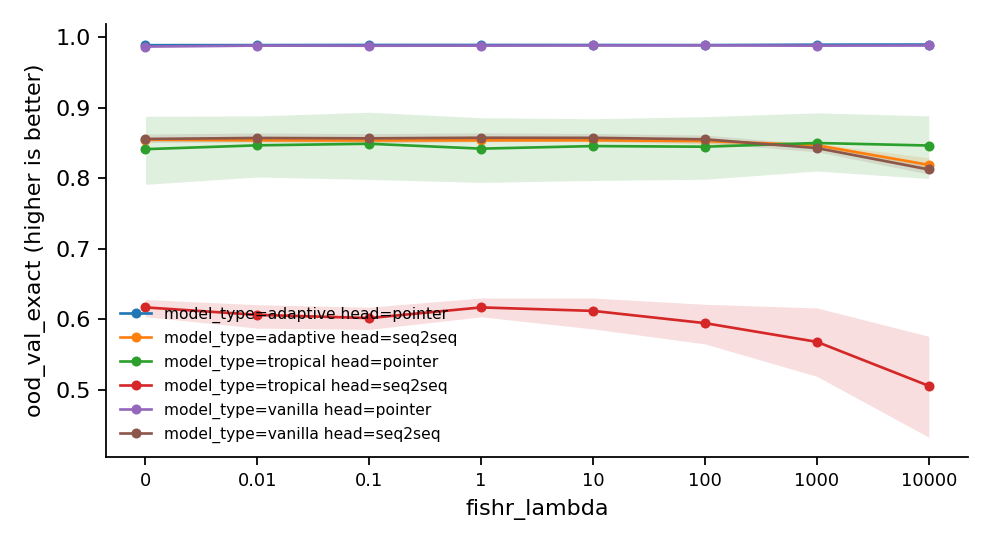
\includegraphics[width=\textwidth]{metric_ood_val_exact.png}
\caption{\texttt{ood\_val\_exact} against \texttt{fishr\_lambda}: the mean over seeds with a 95\% bootstrap CI, one line per combination of the other factors.}
\label{fig:ood_val_exact}
\end{figure}

{\small
\begin{longtable}{lllrlrrr}
\caption{\texttt{ood\_val\_exact} per cell: mean, 95\% bootstrap CI, SD, seeds, diverged runs.}\label{tab:summary-ood_val_exact}\\
\toprule
\texttt{model\_type} & \texttt{head} & \texttt{fishr\_lambda} & mean & 95\% CI & SD & $n$ & div.\\
\midrule
\endhead
adaptive & pointer & 0 & 0.9886 & [0.987, 0.991] & 0.00272 & 5 & 0\\
adaptive & pointer & 0.01 & 0.9888 & [0.988, 0.99] & 0.00163 & 5 & 0\\
adaptive & pointer & 0.1 & 0.989 & [0.988, 0.99] & $9.94\times10^{-4}$ & 5 & 0\\
adaptive & pointer & 1 & 0.989 & [0.988, 0.99] & $9.91\times10^{-4}$ & 5 & 0\\
adaptive & pointer & 10 & 0.9889 & [0.988, 0.99] & 0.00111 & 5 & 0\\
adaptive & pointer & 100 & 0.9888 & [0.988, 0.99] & 0.00119 & 5 & 0\\
adaptive & pointer & 1000 & 0.9894 & [0.989, 0.99] & 0.00104 & 5 & 0\\
adaptive & pointer & 1e+04 & 0.9896 & [0.989, 0.99] & $6.07\times10^{-4}$ & 5 & 0\\
adaptive & seq2seq & 0 & 0.8549 & [0.852, 0.857] & 0.00321 & 5 & 0\\
adaptive & seq2seq & 0.01 & 0.8538 & [0.852, 0.855] & 0.00203 & 5 & 0\\
adaptive & seq2seq & 0.1 & 0.8537 & [0.851, 0.855] & 0.00275 & 5 & 0\\
adaptive & seq2seq & 1 & 0.8539 & [0.852, 0.856] & 0.00236 & 5 & 0\\
adaptive & seq2seq & 10 & 0.8539 & [0.852, 0.855] & 0.00224 & 5 & 0\\
adaptive & seq2seq & 100 & 0.8528 & [0.849, 0.857] & 0.00533 & 5 & 0\\
adaptive & seq2seq & 1000 & 0.8469 & [0.844, 0.849] & 0.00328 & 5 & 0\\
adaptive & seq2seq & 1e+04 & 0.8191 & [0.81, 0.829] & 0.0121 & 5 & 0\\
tropical & pointer & 0 & 0.8413 & [0.791, 0.888] & 0.0634 & 5 & 0\\
tropical & pointer & 0.01 & 0.8467 & [0.802, 0.888] & 0.0579 & 5 & 0\\
tropical & pointer & 0.1 & 0.849 & [0.798, 0.894] & 0.0623 & 5 & 0\\
tropical & pointer & 1 & 0.8421 & [0.794, 0.886] & 0.0572 & 5 & 0\\
tropical & pointer & 10 & 0.8457 & [0.797, 0.884] & 0.0561 & 5 & 0\\
tropical & pointer & 100 & 0.8448 & [0.799, 0.887] & 0.0587 & 5 & 0\\
tropical & pointer & 1000 & 0.85 & [0.81, 0.893] & 0.0541 & 5 & 0\\
tropical & pointer & 1e+04 & 0.8465 & [0.8, 0.889] & 0.0562 & 5 & 0\\
tropical & seq2seq & 0 & 0.6171 & [0.604, 0.628] & 0.0158 & 5 & 0\\
tropical & seq2seq & 0.01 & 0.6065 & [0.588, 0.621] & 0.0222 & 5 & 0\\
tropical & seq2seq & 0.1 & 0.602 & [0.586, 0.617] & 0.0209 & 5 & 0\\
tropical & seq2seq & 1 & 0.6171 & [0.604, 0.63] & 0.0175 & 5 & 0\\
tropical & seq2seq & 10 & 0.6121 & [0.587, 0.63] & 0.0283 & 5 & 0\\
tropical & seq2seq & 100 & 0.5948 & [0.565, 0.621] & 0.0362 & 5 & 0\\
tropical & seq2seq & 1000 & 0.5683 & [0.519, 0.616] & 0.0621 & 5 & 0\\
tropical & seq2seq & 1e+04 & 0.5059 & [0.433, 0.576] & 0.0939 & 5 & 0\\
vanilla & pointer & 0 & 0.9867 & [0.986, 0.988] & 0.00116 & 5 & 0\\
vanilla & pointer & 0.01 & 0.988 & [0.987, 0.989] & 0.00134 & 5 & 0\\
vanilla & pointer & 0.1 & 0.9878 & [0.987, 0.989] & 0.00106 & 5 & 0\\
vanilla & pointer & 1 & 0.988 & [0.987, 0.989] & 0.0012 & 5 & 0\\
vanilla & pointer & 10 & 0.9883 & [0.988, 0.989] & 0.00115 & 5 & 0\\
vanilla & pointer & 100 & 0.9883 & [0.988, 0.989] & 0.0011 & 5 & 0\\
vanilla & pointer & 1000 & 0.988 & [0.987, 0.989] & 0.0011 & 5 & 0\\
vanilla & pointer & 1e+04 & 0.9882 & [0.988, 0.989] & $6.96\times10^{-4}$ & 5 & 0\\
vanilla & seq2seq & 0 & 0.8558 & [0.851, 0.863] & 0.00769 & 5 & 0\\
vanilla & seq2seq & 0.01 & 0.8572 & [0.851, 0.864] & 0.00829 & 5 & 0\\
vanilla & seq2seq & 0.1 & 0.8567 & [0.851, 0.863] & 0.0083 & 5 & 0\\
vanilla & seq2seq & 1 & 0.8575 & [0.852, 0.864] & 0.00854 & 5 & 0\\
vanilla & seq2seq & 10 & 0.8574 & [0.853, 0.863] & 0.00735 & 5 & 0\\
vanilla & seq2seq & 100 & 0.8553 & [0.85, 0.861] & 0.00705 & 5 & 0\\
vanilla & seq2seq & 1000 & 0.8429 & [0.838, 0.848] & 0.00659 & 5 & 0\\
vanilla & seq2seq & 1e+04 & 0.8126 & [0.806, 0.819] & 0.00862 & 5 & 0\\
\bottomrule
\end{longtable}
}

{\small
\begin{longtable}{lllrrrl}
\caption{\texttt{ood\_val\_exact}: each level of \texttt{fishr\_lambda} against its control (0), within each combination of the other factors. parametric: Dunnett vs control.}\label{tab:control-ood_val_exact}\\
\toprule
\texttt{model\_type} & \texttt{head} & \texttt{fishr\_lambda} & difference & 95\% CI & $p$ & \\
\midrule
\endhead
adaptive & pointer & 0.01 & $1.400\times10^{-4}$ & [-0.00234, 0.00262] & 1.0000 & \\
adaptive & pointer & 0.1 & $3.200\times10^{-4}$ & [-0.00216, 0.0028] & 0.9994 & \\
adaptive & pointer & 1 & $3.200\times10^{-4}$ & [-0.00216, 0.0028] & 0.9994 & \\
adaptive & pointer & 10 & $3.000\times10^{-4}$ & [-0.00218, 0.00278] & 0.9996 & \\
adaptive & pointer & 100 & $1.400\times10^{-4}$ & [-0.00234, 0.00262] & 1.0000 & \\
adaptive & pointer & 1000 & $7.400\times10^{-4}$ & [-0.00174, 0.00322] & 0.9351 & \\
adaptive & pointer & 1e+04 & $9.200\times10^{-4}$ & [-0.00156, 0.0034] & 0.8410 & \\
adaptive & seq2seq & 0.01 & -0.00112 & [-0.0103, 0.00801] & 0.9996 & \\
adaptive & seq2seq & 0.1 & -0.0012 & [-0.0103, 0.00793] & 0.9994 & \\
adaptive & seq2seq & 1 & -0.00102 & [-0.0102, 0.00811] & 0.9998 & \\
adaptive & seq2seq & 10 & -0.00102 & [-0.0102, 0.00811] & 0.9998 & \\
adaptive & seq2seq & 100 & -0.00206 & [-0.0112, 0.00707] & 0.9839 & \\
adaptive & seq2seq & 1000 & -0.00802 & [-0.0172, 0.00111] & 0.1042 & \\
adaptive & seq2seq & 1e+04 & -0.03582 & [-0.045, -0.0267] & $<10^{-4}$ & *\\
tropical & pointer & 0.01 & 0.00542 & [-0.0964, 0.107] & 1.0000 & \\
tropical & pointer & 0.1 & 0.00764 & [-0.0942, 0.11] & 1.0000 & \\
tropical & pointer & 1 & $7.400\times10^{-4}$ & [-0.101, 0.103] & 1.0000 & \\
tropical & pointer & 10 & 0.00436 & [-0.0975, 0.106] & 1.0000 & \\
tropical & pointer & 100 & 0.00348 & [-0.0984, 0.105] & 1.0000 & \\
tropical & pointer & 1000 & 0.00872 & [-0.0931, 0.111] & 1.0000 & \\
tropical & pointer & 1e+04 & 0.00516 & [-0.0967, 0.107] & 1.0000 & \\
tropical & seq2seq & 0.01 & -0.0106 & [-0.0894, 0.0682] & 0.9993 & \\
tropical & seq2seq & 0.1 & -0.01512 & [-0.0939, 0.0637] & 0.9935 & \\
tropical & seq2seq & 1 & $-4.000\times10^{-5}$ & [-0.0788, 0.0787] & 1.0000 & \\
tropical & seq2seq & 10 & -0.00498 & [-0.0838, 0.0738] & 1.0000 & \\
tropical & seq2seq & 100 & -0.02232 & [-0.101, 0.0565] & 0.9488 & \\
tropical & seq2seq & 1000 & -0.04884 & [-0.128, 0.0299] & 0.3826 & \\
tropical & seq2seq & 1e+04 & -0.1112 & [-0.19, -0.0324] & 0.0029 & *\\
vanilla & pointer & 0.01 & 0.00134 & [$-6.03\times10^{-4}$, 0.00328] & 0.2804 & \\
vanilla & pointer & 0.1 & 0.00114 & [$-8.03\times10^{-4}$, 0.00308] & 0.4389 & \\
vanilla & pointer & 1 & 0.00134 & [$-6.03\times10^{-4}$, 0.00328] & 0.2804 & \\
vanilla & pointer & 10 & 0.00156 & [$-3.83\times10^{-4}$, 0.0035] & 0.1585 & \\
vanilla & pointer & 100 & 0.00164 & [$-3.03\times10^{-4}$, 0.00358] & 0.1266 & \\
vanilla & pointer & 1000 & 0.00128 & [$-6.63\times10^{-4}$, 0.00322] & 0.3232 & \\
vanilla & pointer & 1e+04 & 0.0015 & [$-4.43\times10^{-4}$, 0.00344] & 0.1864 & \\
vanilla & seq2seq & 0.01 & 0.00138 & [-0.0123, 0.0151] & 0.9999 & \\
vanilla & seq2seq & 0.1 & $9.000\times10^{-4}$ & [-0.0128, 0.0146] & 1.0000 & \\
vanilla & seq2seq & 1 & 0.00172 & [-0.012, 0.0154] & 0.9995 & \\
vanilla & seq2seq & 10 & 0.00158 & [-0.0121, 0.0153] & 0.9997 & \\
vanilla & seq2seq & 100 & $-5.000\times10^{-4}$ & [-0.0142, 0.0132] & 1.0000 & \\
vanilla & seq2seq & 1000 & -0.0129 & [-0.0266, $7.87\times10^{-4}$] & 0.0712 & \\
vanilla & seq2seq & 1e+04 & -0.04322 & [-0.0569, -0.0295] & $<10^{-4}$ & *\\
\bottomrule
\end{longtable}
}

{\small
\begin{longtable}{llrrrrr}
\caption{\texttt{ood\_val\_exact} against log10 \texttt{fishr\_lambda}: parametric: OLS slope t-test, seed-bootstrap CI, with the Jonckheere--Terpstra ordered-trend $\tau$ and $p$.}\label{tab:trend-ood_val_exact}\\
\toprule
\texttt{model\_type} & \texttt{head} & estimate & 95\% CI & $p$ & JT $\tau$ & JT $p$\\
\midrule
\endhead
adaptive & pointer & $1.071\times10^{-4}$ & [$-7.86\times10^{-6}$, $2.22\times10^{-4}$] & 0.2337 & 0.135 & 0.3139\\
adaptive & seq2seq & -0.004242 & [-0.00523, -0.00307] & $<10^{-4}$ & -0.501 & 0.0004\\
tropical & pointer & $1.471\times10^{-4}$ & [$-9.05\times10^{-4}$, $8.58\times10^{-4}$] & 0.9740 & 0.00571 & 0.9758\\
tropical & seq2seq & -0.01398 & [-0.0235, -0.00515] & 0.0022 & -0.299 & 0.0258\\
vanilla & pointer & $3.786\times10^{-5}$ & [$-2.86\times10^{-5}$, $1.34\times10^{-4}$] & 0.6663 & 0.0781 & 0.5603\\
vanilla & seq2seq & -0.005844 & [-0.00645, -0.0052] & $<10^{-4}$ & -0.528 & 0.0004\\
\bottomrule
\end{longtable}
}

{\small
\begin{longtable}{lrrrl}
\caption{\texttt{ood\_val\_exact}: paired contrasts by seed, Holm-corrected across the cells. parametric: paired t-test by seed, Holm.}\label{tab:paired-ood_val_exact}\\
\toprule
contrast (within) & difference & 95\% CI & $p$ & \\
\midrule
\endhead
\stackcell{model\_type: tropical - vanilla\\\footnotesize head=pointer fishr\_lambda=0 } & -0.1454 & [-0.225, -0.0659] & 0.0401 & *\\
\stackcell{model\_type: tropical - vanilla\\\footnotesize head=pointer fishr\_lambda=0.01 } & -0.1413 & [-0.215, -0.0679] & 0.0401 & *\\
\stackcell{model\_type: tropical - vanilla\\\footnotesize head=pointer fishr\_lambda=0.1 } & -0.1389 & [-0.218, -0.0603] & 0.0401 & *\\
\stackcell{model\_type: tropical - vanilla\\\footnotesize head=pointer fishr\_lambda=1 } & -0.146 & [-0.218, -0.0735] & 0.0401 & *\\
\stackcell{model\_type: tropical - vanilla\\\footnotesize head=pointer fishr\_lambda=10 } & -0.1426 & [-0.214, -0.0716] & 0.0401 & *\\
\stackcell{model\_type: tropical - vanilla\\\footnotesize head=pointer fishr\_lambda=100 } & -0.1435 & [-0.218, -0.0693] & 0.0401 & *\\
\stackcell{model\_type: tropical - vanilla\\\footnotesize head=pointer fishr\_lambda=1000 } & -0.1379 & [-0.206, -0.0695] & 0.0401 & *\\
\stackcell{model\_type: tropical - vanilla\\\footnotesize head=pointer fishr\_lambda=1e+04 } & -0.1417 & [-0.212, -0.0711] & 0.0401 & *\\
\stackcell{model\_type: tropical - vanilla\\\footnotesize head=seq2seq fishr\_lambda=0 } & -0.2387 & [-0.267, -0.211] & 0.0003 & *\\
\stackcell{model\_type: tropical - vanilla\\\footnotesize head=seq2seq fishr\_lambda=0.01 } & -0.2506 & [-0.287, -0.215] & 0.0005 & *\\
\stackcell{model\_type: tropical - vanilla\\\footnotesize head=seq2seq fishr\_lambda=0.1 } & -0.2547 & [-0.287, -0.222] & 0.0004 & *\\
\stackcell{model\_type: tropical - vanilla\\\footnotesize head=seq2seq fishr\_lambda=1 } & -0.2404 & [-0.268, -0.213] & 0.0003 & *\\
\stackcell{model\_type: tropical - vanilla\\\footnotesize head=seq2seq fishr\_lambda=10 } & -0.2452 & [-0.289, -0.201] & 0.0011 & *\\
\stackcell{model\_type: tropical - vanilla\\\footnotesize head=seq2seq fishr\_lambda=100 } & -0.2605 & [-0.306, -0.215] & 0.0011 & *\\
\stackcell{model\_type: tropical - vanilla\\\footnotesize head=seq2seq fishr\_lambda=1000 } & -0.2746 & [-0.353, -0.197] & 0.0062 & *\\
\stackcell{model\_type: tropical - vanilla\\\footnotesize head=seq2seq fishr\_lambda=1e+04 } & -0.3067 & [-0.424, -0.189] & 0.0172 & *\\
\stackcell{model\_type: adaptive - vanilla\\\footnotesize head=pointer fishr\_lambda=0 } & 0.00194 & [-0.00103, 0.00491] & 1.0000 & \\
\stackcell{model\_type: adaptive - vanilla\\\footnotesize head=pointer fishr\_lambda=0.01 } & $7.400\times10^{-4}$ & [-0.00139, 0.00287] & 1.0000 & \\
\stackcell{model\_type: adaptive - vanilla\\\footnotesize head=pointer fishr\_lambda=0.1 } & 0.00112 & [$-2.61\times10^{-4}$, 0.0025] & 1.0000 & \\
\stackcell{model\_type: adaptive - vanilla\\\footnotesize head=pointer fishr\_lambda=1 } & $9.200\times10^{-4}$ & [$-3.51\times10^{-4}$, 0.00219] & 1.0000 & \\
\stackcell{model\_type: adaptive - vanilla\\\footnotesize head=pointer fishr\_lambda=10 } & $6.800\times10^{-4}$ & [$-4.22\times10^{-4}$, 0.00178] & 1.0000 & \\
\stackcell{model\_type: adaptive - vanilla\\\footnotesize head=pointer fishr\_lambda=100 } & $4.400\times10^{-4}$ & [-0.00149, 0.00237] & 1.0000 & \\
\stackcell{model\_type: adaptive - vanilla\\\footnotesize head=pointer fishr\_lambda=1000 } & 0.0014 & [$-1.97\times10^{-4}$, 0.003] & 1.0000 & \\
\stackcell{model\_type: adaptive - vanilla\\\footnotesize head=pointer fishr\_lambda=1e+04 } & 0.00136 & [$4.71\times10^{-4}$, 0.00225] & 0.2112 & \\
\stackcell{model\_type: adaptive - vanilla\\\footnotesize head=seq2seq fishr\_lambda=0 } & $-9.000\times10^{-4}$ & [-0.00876, 0.00696] & 1.0000 & \\
\stackcell{model\_type: adaptive - vanilla\\\footnotesize head=seq2seq fishr\_lambda=0.01 } & -0.0034 & [-0.0113, 0.00453] & 1.0000 & \\
\stackcell{model\_type: adaptive - vanilla\\\footnotesize head=seq2seq fishr\_lambda=0.1 } & -0.003 & [-0.0108, 0.00477] & 1.0000 & \\
\stackcell{model\_type: adaptive - vanilla\\\footnotesize head=seq2seq fishr\_lambda=1 } & -0.00364 & [-0.0118, 0.00456] & 1.0000 & \\
\stackcell{model\_type: adaptive - vanilla\\\footnotesize head=seq2seq fishr\_lambda=10 } & -0.0035 & [-0.0108, 0.00375] & 1.0000 & \\
\stackcell{model\_type: adaptive - vanilla\\\footnotesize head=seq2seq fishr\_lambda=100 } & -0.00246 & [-0.00701, 0.00209] & 1.0000 & \\
\stackcell{model\_type: adaptive - vanilla\\\footnotesize head=seq2seq fishr\_lambda=1000 } & 0.00398 & [-0.00243, 0.0104] & 1.0000 & \\
\stackcell{model\_type: adaptive - vanilla\\\footnotesize head=seq2seq fishr\_lambda=1e+04 } & 0.0065 & [-0.00284, 0.0158] & 1.0000 & \\
\stackcell{head: pointer - seq2seq\\\footnotesize model\_type=adaptive fishr\_lambda=0 } & 0.1338 & [0.127, 0.141] & $<10^{-4}$ & *\\
\stackcell{head: pointer - seq2seq\\\footnotesize model\_type=adaptive fishr\_lambda=0.01 } & 0.135 & [0.133, 0.137] & $<10^{-4}$ & *\\
\stackcell{head: pointer - seq2seq\\\footnotesize model\_type=adaptive fishr\_lambda=0.1 } & 0.1353 & [0.132, 0.138] & $<10^{-4}$ & *\\
\stackcell{head: pointer - seq2seq\\\footnotesize model\_type=adaptive fishr\_lambda=1 } & 0.1351 & [0.132, 0.138] & $<10^{-4}$ & *\\
\stackcell{head: pointer - seq2seq\\\footnotesize model\_type=adaptive fishr\_lambda=10 } & 0.1351 & [0.133, 0.138] & $<10^{-4}$ & *\\
\stackcell{head: pointer - seq2seq\\\footnotesize model\_type=adaptive fishr\_lambda=100 } & 0.136 & [0.13, 0.142] & $<10^{-4}$ & *\\
\stackcell{head: pointer - seq2seq\\\footnotesize model\_type=adaptive fishr\_lambda=1000 } & 0.1425 & [0.139, 0.146] & $<10^{-4}$ & *\\
\stackcell{head: pointer - seq2seq\\\footnotesize model\_type=adaptive fishr\_lambda=1e+04 } & 0.1705 & [0.156, 0.185] & $<10^{-4}$ & *\\
\stackcell{head: pointer - seq2seq\\\footnotesize model\_type=tropical fishr\_lambda=0 } & 0.2242 & [0.131, 0.318] & 0.0128 & *\\
\stackcell{head: pointer - seq2seq\\\footnotesize model\_type=tropical fishr\_lambda=0.01 } & 0.2402 & [0.152, 0.328] & 0.0121 & *\\
\stackcell{head: pointer - seq2seq\\\footnotesize model\_type=tropical fishr\_lambda=0.1 } & 0.247 & [0.158, 0.336] & 0.0121 & *\\
\stackcell{head: pointer - seq2seq\\\footnotesize model\_type=tropical fishr\_lambda=1 } & 0.225 & [0.135, 0.315] & 0.0128 & *\\
\stackcell{head: pointer - seq2seq\\\footnotesize model\_type=tropical fishr\_lambda=10 } & 0.2335 & [0.14, 0.327] & 0.0128 & *\\
\stackcell{head: pointer - seq2seq\\\footnotesize model\_type=tropical fishr\_lambda=100 } & 0.25 & [0.152, 0.348] & 0.0128 & *\\
\stackcell{head: pointer - seq2seq\\\footnotesize model\_type=tropical fishr\_lambda=1000 } & 0.2818 & [0.153, 0.411] & 0.0128 & *\\
\stackcell{head: pointer - seq2seq\\\footnotesize model\_type=tropical fishr\_lambda=1e+04 } & 0.3406 & [0.18, 0.501] & 0.0128 & *\\
\stackcell{head: pointer - seq2seq\\\footnotesize model\_type=vanilla fishr\_lambda=0 } & 0.1309 & [0.121, 0.141] & $<10^{-4}$ & *\\
\stackcell{head: pointer - seq2seq\\\footnotesize model\_type=vanilla fishr\_lambda=0.01 } & 0.1309 & [0.12, 0.142] & $<10^{-4}$ & *\\
\stackcell{head: pointer - seq2seq\\\footnotesize model\_type=vanilla fishr\_lambda=0.1 } & 0.1312 & [0.12, 0.142] & $<10^{-4}$ & *\\
\stackcell{head: pointer - seq2seq\\\footnotesize model\_type=vanilla fishr\_lambda=1 } & 0.1305 & [0.119, 0.142] & $<10^{-4}$ & *\\
\stackcell{head: pointer - seq2seq\\\footnotesize model\_type=vanilla fishr\_lambda=10 } & 0.1309 & [0.121, 0.141] & $<10^{-4}$ & *\\
\stackcell{head: pointer - seq2seq\\\footnotesize model\_type=vanilla fishr\_lambda=100 } & 0.1331 & [0.123, 0.143] & $<10^{-4}$ & *\\
\stackcell{head: pointer - seq2seq\\\footnotesize model\_type=vanilla fishr\_lambda=1000 } & 0.1451 & [0.136, 0.154] & $<10^{-4}$ & *\\
\stackcell{head: pointer - seq2seq\\\footnotesize model\_type=vanilla fishr\_lambda=1e+04 } & 0.1756 & [0.164, 0.187] & $<10^{-4}$ & *\\
\bottomrule
\end{longtable}
}

\subsection{\texttt{ood\_noise\_f1}}
\begin{figure}[tbp]
\centering
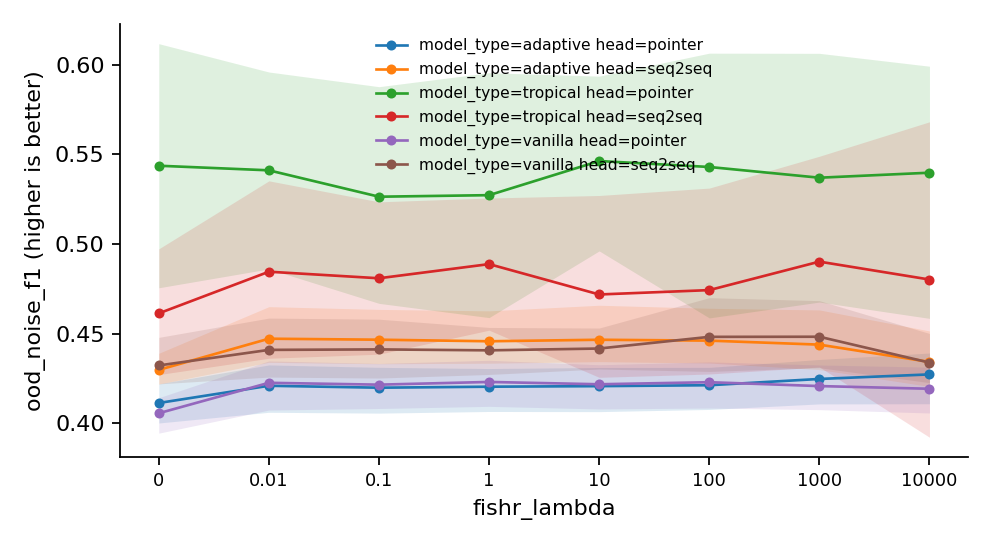
\includegraphics[width=\textwidth]{metric_ood_noise_f1.png}
\caption{\texttt{ood\_noise\_f1} against \texttt{fishr\_lambda}: the mean over seeds with a 95\% bootstrap CI, one line per combination of the other factors.}
\label{fig:ood_noise_f1}
\end{figure}

{\small
\begin{longtable}{lllrlrrr}
\caption{\texttt{ood\_noise\_f1} per cell: mean, 95\% bootstrap CI, SD, seeds, diverged runs.}\label{tab:summary-ood_noise_f1}\\
\toprule
\texttt{model\_type} & \texttt{head} & \texttt{fishr\_lambda} & mean & 95\% CI & SD & $n$ & div.\\
\midrule
\endhead
adaptive & pointer & 0 & 0.4113 & [0.4, 0.422] & 0.0142 & 5 & 0\\
adaptive & pointer & 0.01 & 0.4209 & [0.406, 0.433] & 0.0178 & 5 & 0\\
adaptive & pointer & 0.1 & 0.4198 & [0.406, 0.431] & 0.0165 & 5 & 0\\
adaptive & pointer & 1 & 0.4204 & [0.407, 0.431] & 0.0163 & 5 & 0\\
adaptive & pointer & 10 & 0.4207 & [0.406, 0.431] & 0.0161 & 5 & 0\\
adaptive & pointer & 100 & 0.4212 & [0.408, 0.431] & 0.0159 & 5 & 0\\
adaptive & pointer & 1000 & 0.4247 & [0.411, 0.436] & 0.0165 & 5 & 0\\
adaptive & pointer & 1e+04 & 0.4272 & [0.411, 0.439] & 0.0181 & 5 & 0\\
adaptive & seq2seq & 0 & 0.4298 & [0.422, 0.439] & 0.0117 & 5 & 0\\
adaptive & seq2seq & 0.01 & 0.4472 & [0.434, 0.465] & 0.0206 & 5 & 0\\
adaptive & seq2seq & 0.1 & 0.4466 & [0.433, 0.464] & 0.0201 & 5 & 0\\
adaptive & seq2seq & 1 & 0.4457 & [0.433, 0.463] & 0.0189 & 5 & 0\\
adaptive & seq2seq & 10 & 0.4466 & [0.434, 0.466] & 0.0214 & 5 & 0\\
adaptive & seq2seq & 100 & 0.4461 & [0.434, 0.464] & 0.0184 & 5 & 0\\
adaptive & seq2seq & 1000 & 0.4438 & [0.43, 0.463] & 0.022 & 5 & 0\\
adaptive & seq2seq & 1e+04 & 0.4342 & [0.421, 0.451] & 0.0205 & 5 & 0\\
tropical & pointer & 0 & 0.5436 & [0.476, 0.612] & 0.0859 & 5 & 0\\
tropical & pointer & 0.01 & 0.5411 & [0.486, 0.596] & 0.0716 & 5 & 0\\
tropical & pointer & 0.1 & 0.5264 & [0.467, 0.588] & 0.0782 & 5 & 0\\
tropical & pointer & 1 & 0.5272 & [0.459, 0.596] & 0.0896 & 5 & 0\\
tropical & pointer & 10 & 0.5463 & [0.496, 0.594] & 0.0634 & 5 & 0\\
tropical & pointer & 100 & 0.543 & [0.459, 0.606] & 0.0938 & 5 & 0\\
tropical & pointer & 1000 & 0.537 & [0.468, 0.606] & 0.0875 & 5 & 0\\
tropical & pointer & 1e+04 & 0.5398 & [0.458, 0.599] & 0.0912 & 5 & 0\\
tropical & seq2seq & 0 & 0.4613 & [0.427, 0.497] & 0.0464 & 5 & 0\\
tropical & seq2seq & 0.01 & 0.4845 & [0.436, 0.535] & 0.0607 & 5 & 0\\
tropical & seq2seq & 0.1 & 0.4809 & [0.439, 0.524] & 0.0538 & 5 & 0\\
tropical & seq2seq & 1 & 0.4888 & [0.452, 0.526] & 0.0474 & 5 & 0\\
tropical & seq2seq & 10 & 0.4718 & [0.426, 0.527] & 0.0605 & 5 & 0\\
tropical & seq2seq & 100 & 0.4743 & [0.427, 0.531] & 0.0704 & 5 & 0\\
tropical & seq2seq & 1000 & 0.4901 & [0.431, 0.549] & 0.0767 & 5 & 0\\
tropical & seq2seq & 1e+04 & 0.4802 & [0.392, 0.568] & 0.113 & 5 & 0\\
vanilla & pointer & 0 & 0.4056 & [0.394, 0.414] & 0.0127 & 5 & 0\\
vanilla & pointer & 0.01 & 0.4225 & [0.407, 0.435] & 0.0176 & 5 & 0\\
vanilla & pointer & 0.1 & 0.4215 & [0.408, 0.433] & 0.0165 & 5 & 0\\
vanilla & pointer & 1 & 0.423 & [0.409, 0.435] & 0.0167 & 5 & 0\\
vanilla & pointer & 10 & 0.4217 & [0.408, 0.433] & 0.016 & 5 & 0\\
vanilla & pointer & 100 & 0.4229 & [0.408, 0.434] & 0.017 & 5 & 0\\
vanilla & pointer & 1000 & 0.4207 & [0.408, 0.432] & 0.0168 & 5 & 0\\
vanilla & pointer & 1e+04 & 0.4192 & [0.406, 0.431] & 0.0171 & 5 & 0\\
vanilla & seq2seq & 0 & 0.4322 & [0.422, 0.448] & 0.0166 & 5 & 0\\
vanilla & seq2seq & 0.01 & 0.4409 & [0.426, 0.459] & 0.0216 & 5 & 0\\
vanilla & seq2seq & 0.1 & 0.4412 & [0.425, 0.458] & 0.0206 & 5 & 0\\
vanilla & seq2seq & 1 & 0.4407 & [0.427, 0.453] & 0.0173 & 5 & 0\\
vanilla & seq2seq & 10 & 0.4417 & [0.43, 0.453] & 0.0153 & 5 & 0\\
vanilla & seq2seq & 100 & 0.4482 & [0.429, 0.47] & 0.0257 & 5 & 0\\
vanilla & seq2seq & 1000 & 0.4482 & [0.431, 0.468] & 0.0254 & 5 & 0\\
vanilla & seq2seq & 1e+04 & 0.4338 & [0.423, 0.45] & 0.018 & 5 & 0\\
\bottomrule
\end{longtable}
}

{\small
\begin{longtable}{lllrrrl}
\caption{\texttt{ood\_noise\_f1}: each level of \texttt{fishr\_lambda} against its control (0), within each combination of the other factors. parametric: Dunnett vs control.}\label{tab:control-ood_noise_f1}\\
\toprule
\texttt{model\_type} & \texttt{head} & \texttt{fishr\_lambda} & difference & 95\% CI & $p$ & \\
\midrule
\endhead
adaptive & pointer & 0.01 & 0.009602 & [-0.0192, 0.0384] & 0.8945 & \\
adaptive & pointer & 0.1 & 0.008526 & [-0.0202, 0.0373] & 0.9370 & \\
adaptive & pointer & 1 & 0.009082 & [-0.0197, 0.0379] & 0.9166 & \\
adaptive & pointer & 10 & 0.009397 & [-0.0194, 0.0382] & 0.9036 & \\
adaptive & pointer & 100 & 0.009906 & [-0.0189, 0.0387] & 0.8803 & \\
adaptive & pointer & 1000 & 0.0134 & [-0.0154, 0.0422] & 0.6685 & \\
adaptive & pointer & 1e+04 & 0.01594 & [-0.0128, 0.0447] & 0.4981 & \\
adaptive & seq2seq & 0.01 & 0.01738 & [-0.0166, 0.0513] & 0.5785 & \\
adaptive & seq2seq & 0.1 & 0.01682 & [-0.0171, 0.0508] & 0.6107 & \\
adaptive & seq2seq & 1 & 0.01594 & [-0.018, 0.0499] & 0.6611 & \\
adaptive & seq2seq & 10 & 0.01679 & [-0.0172, 0.0508] & 0.6122 & \\
adaptive & seq2seq & 100 & 0.0163 & [-0.0177, 0.0503] & 0.6403 & \\
adaptive & seq2seq & 1000 & 0.01407 & [-0.0199, 0.048] & 0.7666 & \\
adaptive & seq2seq & 1e+04 & 0.004418 & [-0.0295, 0.0384] & 0.9994 & \\
tropical & pointer & 0.01 & -0.002559 & [-0.148, 0.143] & 1.0000 & \\
tropical & pointer & 0.1 & -0.01728 & [-0.163, 0.128] & 0.9997 & \\
tropical & pointer & 1 & -0.01642 & [-0.162, 0.129] & 0.9998 & \\
tropical & pointer & 10 & 0.002618 & [-0.143, 0.148] & 1.0000 & \\
tropical & pointer & 100 & $-6.931\times10^{-4}$ & [-0.146, 0.145] & 1.0000 & \\
tropical & pointer & 1000 & -0.006681 & [-0.152, 0.139] & 1.0000 & \\
tropical & pointer & 1e+04 & -0.003891 & [-0.149, 0.142] & 1.0000 & \\
tropical & seq2seq & 0.01 & 0.02323 & [-0.0975, 0.144] & 0.9934 & \\
tropical & seq2seq & 0.1 & 0.01958 & [-0.101, 0.14] & 0.9976 & \\
tropical & seq2seq & 1 & 0.02748 & [-0.0933, 0.148] & 0.9831 & \\
tropical & seq2seq & 10 & 0.01054 & [-0.11, 0.131] & 1.0000 & \\
tropical & seq2seq & 100 & 0.01297 & [-0.108, 0.134] & 0.9998 & \\
tropical & seq2seq & 1000 & 0.02886 & [-0.0919, 0.15] & 0.9781 & \\
tropical & seq2seq & 1e+04 & 0.01887 & [-0.102, 0.14] & 0.9981 & \\
vanilla & pointer & 0.01 & 0.01697 & [-0.0116, 0.0455] & 0.4260 & \\
vanilla & pointer & 0.1 & 0.01593 & [-0.0126, 0.0445] & 0.4906 & \\
vanilla & pointer & 1 & 0.01745 & [-0.0111, 0.046] & 0.3975 & \\
vanilla & pointer & 10 & 0.01616 & [-0.0124, 0.0447] & 0.4763 & \\
vanilla & pointer & 100 & 0.0173 & [-0.0113, 0.0459] & 0.4060 & \\
vanilla & pointer & 1000 & 0.01515 & [-0.0134, 0.0437] & 0.5424 & \\
vanilla & pointer & 1e+04 & 0.01365 & [-0.0149, 0.0422] & 0.6446 & \\
vanilla & seq2seq & 0.01 & 0.00869 & [-0.027, 0.0443] & 0.9757 & \\
vanilla & seq2seq & 0.1 & 0.008957 & [-0.0267, 0.0446] & 0.9716 & \\
vanilla & seq2seq & 1 & 0.008433 & [-0.0272, 0.0441] & 0.9792 & \\
vanilla & seq2seq & 10 & 0.009445 & [-0.0262, 0.0451] & 0.9629 & \\
vanilla & seq2seq & 100 & 0.01595 & [-0.0197, 0.0516] & 0.7035 & \\
vanilla & seq2seq & 1000 & 0.01602 & [-0.0196, 0.0517] & 0.6999 & \\
vanilla & seq2seq & 1e+04 & 0.001594 & [-0.034, 0.0372] & 1.0000 & \\
\bottomrule
\end{longtable}
}

{\small
\begin{longtable}{llrrrrr}
\caption{\texttt{ood\_noise\_f1} against log10 \texttt{fishr\_lambda}: parametric: OLS slope t-test, seed-bootstrap CI, with the Jonckheere--Terpstra ordered-trend $\tau$ and $p$.}\label{tab:trend-ood_noise_f1}\\
\toprule
\texttt{model\_type} & \texttt{head} & estimate & 95\% CI & $p$ & JT $\tau$ & JT $p$\\
\midrule
\endhead
adaptive & pointer & 0.001056 & [$5.20\times10^{-4}$, 0.00159] & 0.4265 & 0.23 & 0.0832\\
adaptive & seq2seq & -0.001572 & [-0.00237, $-6.92\times10^{-4}$] & 0.3331 & -0.181 & 0.1796\\
tropical & pointer & 0.001176 & [-0.00454, 0.00677] & 0.8570 & 0.0362 & 0.8072\\
tropical & seq2seq & $-3.221\times10^{-4}$ & [-0.0125, 0.0109] & 0.9546 & -0.0286 & 0.8454\\
vanilla & pointer & $-4.170\times10^{-4}$ & [-0.00144, $4.81\times10^{-4}$] & 0.7525 & -0.0667 & 0.6267\\
vanilla & seq2seq & $1.307\times10^{-5}$ & [-0.00219, 0.00206] & 0.9938 & -0.0438 & 0.7441\\
\bottomrule
\end{longtable}
}

{\small
\begin{longtable}{lrrrl}
\caption{\texttt{ood\_noise\_f1}: paired contrasts by seed, Holm-corrected across the cells. parametric: paired t-test by seed, Holm.}\label{tab:paired-ood_noise_f1}\\
\toprule
contrast (within) & difference & 95\% CI & $p$ & \\
\midrule
\endhead
\stackcell{model\_type: tropical - vanilla\\\footnotesize head=pointer fishr\_lambda=0 } & 0.1381 & [0.0177, 0.258] & 0.5007 & \\
\stackcell{model\_type: tropical - vanilla\\\footnotesize head=pointer fishr\_lambda=0.01 } & 0.1185 & [0.0143, 0.223] & 0.5007 & \\
\stackcell{model\_type: tropical - vanilla\\\footnotesize head=pointer fishr\_lambda=0.1 } & 0.1049 & [-0.00719, 0.217] & 0.6342 & \\
\stackcell{model\_type: tropical - vanilla\\\footnotesize head=pointer fishr\_lambda=1 } & 0.1042 & [-0.0216, 0.23] & 0.7460 & \\
\stackcell{model\_type: tropical - vanilla\\\footnotesize head=pointer fishr\_lambda=10 } & 0.1245 & [0.0332, 0.216] & 0.3093 & \\
\stackcell{model\_type: tropical - vanilla\\\footnotesize head=pointer fishr\_lambda=100 } & 0.1201 & [-0.00238, 0.243] & 0.6342 & \\
\stackcell{model\_type: tropical - vanilla\\\footnotesize head=pointer fishr\_lambda=1000 } & 0.1162 & [-0.00345, 0.236] & 0.6342 & \\
\stackcell{model\_type: tropical - vanilla\\\footnotesize head=pointer fishr\_lambda=1e+04 } & 0.1205 & [0.00372, 0.237] & 0.5942 & \\
\stackcell{model\_type: tropical - vanilla\\\footnotesize head=seq2seq fishr\_lambda=0 } & 0.02906 & [-0.0397, 0.0978] & 1.0000 & \\
\stackcell{model\_type: tropical - vanilla\\\footnotesize head=seq2seq fishr\_lambda=0.01 } & 0.0436 & [-0.0401, 0.127] & 1.0000 & \\
\stackcell{model\_type: tropical - vanilla\\\footnotesize head=seq2seq fishr\_lambda=0.1 } & 0.03968 & [-0.0327, 0.112] & 1.0000 & \\
\stackcell{model\_type: tropical - vanilla\\\footnotesize head=seq2seq fishr\_lambda=1 } & 0.04811 & [-0.0187, 0.115] & 0.9310 & \\
\stackcell{model\_type: tropical - vanilla\\\footnotesize head=seq2seq fishr\_lambda=10 } & 0.03015 & [-0.0575, 0.118] & 1.0000 & \\
\stackcell{model\_type: tropical - vanilla\\\footnotesize head=seq2seq fishr\_lambda=100 } & 0.02608 & [-0.052, 0.104] & 1.0000 & \\
\stackcell{model\_type: tropical - vanilla\\\footnotesize head=seq2seq fishr\_lambda=1000 } & 0.0419 & [-0.0441, 0.128] & 1.0000 & \\
\stackcell{model\_type: tropical - vanilla\\\footnotesize head=seq2seq fishr\_lambda=1e+04 } & 0.04634 & [-0.0835, 0.176] & 1.0000 & \\
\stackcell{model\_type: adaptive - vanilla\\\footnotesize head=pointer fishr\_lambda=0 } & 0.005718 & [-0.00405, 0.0155] & 1.0000 & \\
\stackcell{model\_type: adaptive - vanilla\\\footnotesize head=pointer fishr\_lambda=0.01 } & -0.001648 & [-0.00827, 0.00497] & 1.0000 & \\
\stackcell{model\_type: adaptive - vanilla\\\footnotesize head=pointer fishr\_lambda=0.1 } & -0.00169 & [-0.00938, 0.006] & 1.0000 & \\
\stackcell{model\_type: adaptive - vanilla\\\footnotesize head=pointer fishr\_lambda=1 } & -0.002649 & [-0.0106, 0.00533] & 1.0000 & \\
\stackcell{model\_type: adaptive - vanilla\\\footnotesize head=pointer fishr\_lambda=10 } & -0.001041 & [-0.00609, 0.004] & 1.0000 & \\
\stackcell{model\_type: adaptive - vanilla\\\footnotesize head=pointer fishr\_lambda=100 } & -0.001677 & [-0.0121, 0.00876] & 1.0000 & \\
\stackcell{model\_type: adaptive - vanilla\\\footnotesize head=pointer fishr\_lambda=1000 } & 0.003972 & [-0.00956, 0.0175] & 1.0000 & \\
\stackcell{model\_type: adaptive - vanilla\\\footnotesize head=pointer fishr\_lambda=1e+04 } & 0.008003 & [-0.00307, 0.0191] & 1.0000 & \\
\stackcell{model\_type: adaptive - vanilla\\\footnotesize head=seq2seq fishr\_lambda=0 } & -0.002449 & [-0.0235, 0.0186] & 1.0000 & \\
\stackcell{model\_type: adaptive - vanilla\\\footnotesize head=seq2seq fishr\_lambda=0.01 } & 0.006237 & [-0.0156, 0.028] & 1.0000 & \\
\stackcell{model\_type: adaptive - vanilla\\\footnotesize head=seq2seq fishr\_lambda=0.1 } & 0.005413 & [-0.0131, 0.0239] & 1.0000 & \\
\stackcell{model\_type: adaptive - vanilla\\\footnotesize head=seq2seq fishr\_lambda=1 } & 0.005062 & [-0.0162, 0.0263] & 1.0000 & \\
\stackcell{model\_type: adaptive - vanilla\\\footnotesize head=seq2seq fishr\_lambda=10 } & 0.004896 & [-0.0205, 0.0302] & 1.0000 & \\
\stackcell{model\_type: adaptive - vanilla\\\footnotesize head=seq2seq fishr\_lambda=100 } & -0.002101 & [-0.0234, 0.0192] & 1.0000 & \\
\stackcell{model\_type: adaptive - vanilla\\\footnotesize head=seq2seq fishr\_lambda=1000 } & -0.004406 & [-0.0203, 0.0115] & 1.0000 & \\
\stackcell{model\_type: adaptive - vanilla\\\footnotesize head=seq2seq fishr\_lambda=1e+04 } & $3.747\times10^{-4}$ & [-0.0125, 0.0132] & 1.0000 & \\
\stackcell{head: pointer - seq2seq\\\footnotesize model\_type=adaptive fishr\_lambda=0 } & -0.01848 & [-0.0409, 0.00398] & 1.0000 & \\
\stackcell{head: pointer - seq2seq\\\footnotesize model\_type=adaptive fishr\_lambda=0.01 } & -0.02626 & [-0.0476, -0.0049] & 0.6176 & \\
\stackcell{head: pointer - seq2seq\\\footnotesize model\_type=adaptive fishr\_lambda=0.1 } & -0.02678 & [-0.0482, -0.00531] & 0.6176 & \\
\stackcell{head: pointer - seq2seq\\\footnotesize model\_type=adaptive fishr\_lambda=1 } & -0.02534 & [-0.0464, -0.00431] & 0.6176 & \\
\stackcell{head: pointer - seq2seq\\\footnotesize model\_type=adaptive fishr\_lambda=10 } & -0.02587 & [-0.0527, $9.86\times10^{-4}$] & 1.0000 & \\
\stackcell{head: pointer - seq2seq\\\footnotesize model\_type=adaptive fishr\_lambda=100 } & -0.02488 & [-0.045, -0.00474] & 0.6176 & \\
\stackcell{head: pointer - seq2seq\\\footnotesize model\_type=adaptive fishr\_lambda=1000 } & -0.01915 & [-0.0435, 0.00521] & 1.0000 & \\
\stackcell{head: pointer - seq2seq\\\footnotesize model\_type=adaptive fishr\_lambda=1e+04 } & -0.006965 & [-0.0301, 0.0162] & 1.0000 & \\
\stackcell{head: pointer - seq2seq\\\footnotesize model\_type=tropical fishr\_lambda=0 } & 0.08236 & [-0.0542, 0.219] & 1.0000 & \\
\stackcell{head: pointer - seq2seq\\\footnotesize model\_type=tropical fishr\_lambda=0.01 } & 0.05657 & [-0.0923, 0.205] & 1.0000 & \\
\stackcell{head: pointer - seq2seq\\\footnotesize model\_type=tropical fishr\_lambda=0.1 } & 0.0455 & [-0.102, 0.193] & 1.0000 & \\
\stackcell{head: pointer - seq2seq\\\footnotesize model\_type=tropical fishr\_lambda=1 } & 0.03846 & [-0.123, 0.2] & 1.0000 & \\
\stackcell{head: pointer - seq2seq\\\footnotesize model\_type=tropical fishr\_lambda=10 } & 0.07444 & [-0.0498, 0.199] & 1.0000 & \\
\stackcell{head: pointer - seq2seq\\\footnotesize model\_type=tropical fishr\_lambda=100 } & 0.06869 & [-0.122, 0.259] & 1.0000 & \\
\stackcell{head: pointer - seq2seq\\\footnotesize model\_type=tropical fishr\_lambda=1000 } & 0.04682 & [-0.149, 0.243] & 1.0000 & \\
\stackcell{head: pointer - seq2seq\\\footnotesize model\_type=tropical fishr\_lambda=1e+04 } & 0.05959 & [-0.171, 0.291] & 1.0000 & \\
\stackcell{head: pointer - seq2seq\\\footnotesize model\_type=vanilla fishr\_lambda=0 } & -0.02665 & [-0.0482, -0.00509] & 0.6176 & \\
\stackcell{head: pointer - seq2seq\\\footnotesize model\_type=vanilla fishr\_lambda=0.01 } & -0.01837 & [-0.0483, 0.0116] & 1.0000 & \\
\stackcell{head: pointer - seq2seq\\\footnotesize model\_type=vanilla fishr\_lambda=0.1 } & -0.01967 & [-0.0498, 0.0104] & 1.0000 & \\
\stackcell{head: pointer - seq2seq\\\footnotesize model\_type=vanilla fishr\_lambda=1 } & -0.01763 & [-0.0467, 0.0114] & 1.0000 & \\
\stackcell{head: pointer - seq2seq\\\footnotesize model\_type=vanilla fishr\_lambda=10 } & -0.01994 & [-0.0427, 0.0028] & 1.0000 & \\
\stackcell{head: pointer - seq2seq\\\footnotesize model\_type=vanilla fishr\_lambda=100 } & -0.0253 & [-0.064, 0.0134] & 1.0000 & \\
\stackcell{head: pointer - seq2seq\\\footnotesize model\_type=vanilla fishr\_lambda=1000 } & -0.02753 & [-0.0675, 0.0124] & 1.0000 & \\
\stackcell{head: pointer - seq2seq\\\footnotesize model\_type=vanilla fishr\_lambda=1e+04 } & -0.01459 & [-0.0439, 0.0147] & 1.0000 & \\
\bottomrule
\end{longtable}
}

\subsection{\texttt{ood\_noise\_exact}}
\begin{figure}[tbp]
\centering
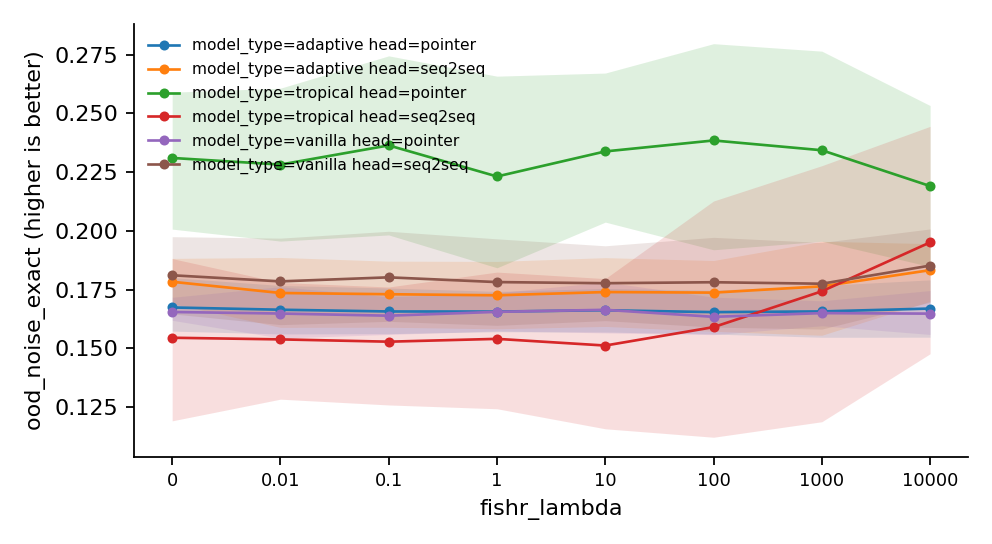
\includegraphics[width=\textwidth]{metric_ood_noise_exact.png}
\caption{\texttt{ood\_noise\_exact} against \texttt{fishr\_lambda}: the mean over seeds with a 95\% bootstrap CI, one line per combination of the other factors.}
\label{fig:ood_noise_exact}
\end{figure}

{\small
\begin{longtable}{lllrlrrr}
\caption{\texttt{ood\_noise\_exact} per cell: mean, 95\% bootstrap CI, SD, seeds, diverged runs.}\label{tab:summary-ood_noise_exact}\\
\toprule
\texttt{model\_type} & \texttt{head} & \texttt{fishr\_lambda} & mean & 95\% CI & SD & $n$ & div.\\
\midrule
\endhead
adaptive & pointer & 0 & 0.1674 & [0.157, 0.18] & 0.0144 & 5 & 0\\
adaptive & pointer & 0.01 & 0.1665 & [0.156, 0.177] & 0.0131 & 5 & 0\\
adaptive & pointer & 0.1 & 0.1657 & [0.156, 0.176] & 0.0127 & 5 & 0\\
adaptive & pointer & 1 & 0.1657 & [0.157, 0.174] & 0.0111 & 5 & 0\\
adaptive & pointer & 10 & 0.1663 & [0.157, 0.176] & 0.0119 & 5 & 0\\
adaptive & pointer & 100 & 0.1655 & [0.156, 0.175] & 0.0118 & 5 & 0\\
adaptive & pointer & 1000 & 0.1658 & [0.155, 0.177] & 0.0141 & 5 & 0\\
adaptive & pointer & 1e+04 & 0.167 & [0.155, 0.179] & 0.0153 & 5 & 0\\
adaptive & seq2seq & 0 & 0.1784 & [0.169, 0.188] & 0.0126 & 5 & 0\\
adaptive & seq2seq & 0.01 & 0.1736 & [0.159, 0.189] & 0.0196 & 5 & 0\\
adaptive & seq2seq & 0.1 & 0.1731 & [0.159, 0.187] & 0.0194 & 5 & 0\\
adaptive & seq2seq & 1 & 0.1726 & [0.158, 0.187] & 0.0195 & 5 & 0\\
adaptive & seq2seq & 10 & 0.174 & [0.159, 0.189] & 0.0202 & 5 & 0\\
adaptive & seq2seq & 100 & 0.1738 & [0.157, 0.187] & 0.0196 & 5 & 0\\
adaptive & seq2seq & 1000 & 0.1764 & [0.156, 0.196] & 0.0255 & 5 & 0\\
adaptive & seq2seq & 1e+04 & 0.1833 & [0.17, 0.195] & 0.0157 & 5 & 0\\
tropical & pointer & 0 & 0.2311 & [0.201, 0.259] & 0.0364 & 5 & 0\\
tropical & pointer & 0.01 & 0.2282 & [0.196, 0.261] & 0.0453 & 5 & 0\\
tropical & pointer & 0.1 & 0.2364 & [0.198, 0.275] & 0.0492 & 5 & 0\\
tropical & pointer & 1 & 0.2232 & [0.184, 0.266] & 0.0547 & 5 & 0\\
tropical & pointer & 10 & 0.2338 & [0.204, 0.267] & 0.0405 & 5 & 0\\
tropical & pointer & 100 & 0.2385 & [0.192, 0.28] & 0.0542 & 5 & 0\\
tropical & pointer & 1000 & 0.2343 & [0.196, 0.276] & 0.0521 & 5 & 0\\
tropical & pointer & 1e+04 & 0.2191 & [0.185, 0.253] & 0.0455 & 5 & 0\\
tropical & seq2seq & 0 & 0.1546 & [0.119, 0.188] & 0.0427 & 5 & 0\\
tropical & seq2seq & 0.01 & 0.1539 & [0.128, 0.178] & 0.0325 & 5 & 0\\
tropical & seq2seq & 0.1 & 0.1529 & [0.126, 0.176] & 0.0317 & 5 & 0\\
tropical & seq2seq & 1 & 0.1541 & [0.124, 0.182] & 0.0373 & 5 & 0\\
tropical & seq2seq & 10 & 0.1512 & [0.116, 0.18] & 0.0399 & 5 & 0\\
tropical & seq2seq & 100 & 0.1591 & [0.112, 0.213] & 0.0674 & 5 & 0\\
tropical & seq2seq & 1000 & 0.1743 & [0.119, 0.228] & 0.0725 & 5 & 0\\
tropical & seq2seq & 1e+04 & 0.1951 & [0.148, 0.245] & 0.0622 & 5 & 0\\
vanilla & pointer & 0 & 0.1655 & [0.162, 0.172] & 0.00691 & 5 & 0\\
vanilla & pointer & 0.01 & 0.1649 & [0.154, 0.176] & 0.0139 & 5 & 0\\
vanilla & pointer & 0.1 & 0.1639 & [0.156, 0.172] & 0.0106 & 5 & 0\\
vanilla & pointer & 1 & 0.1656 & [0.157, 0.174] & 0.0105 & 5 & 0\\
vanilla & pointer & 10 & 0.1664 & [0.157, 0.178] & 0.0142 & 5 & 0\\
vanilla & pointer & 100 & 0.1635 & [0.156, 0.172] & 0.0109 & 5 & 0\\
vanilla & pointer & 1000 & 0.165 & [0.16, 0.17] & 0.00688 & 5 & 0\\
vanilla & pointer & 1e+04 & 0.1648 & [0.156, 0.175] & 0.0116 & 5 & 0\\
vanilla & seq2seq & 0 & 0.1811 & [0.165, 0.198] & 0.0207 & 5 & 0\\
vanilla & seq2seq & 0.01 & 0.1785 & [0.16, 0.197] & 0.0238 & 5 & 0\\
vanilla & seq2seq & 0.1 & 0.1803 & [0.162, 0.2] & 0.0254 & 5 & 0\\
vanilla & seq2seq & 1 & 0.1782 & [0.16, 0.197] & 0.0243 & 5 & 0\\
vanilla & seq2seq & 10 & 0.1778 & [0.162, 0.194] & 0.0213 & 5 & 0\\
vanilla & seq2seq & 100 & 0.1782 & [0.159, 0.197] & 0.0253 & 5 & 0\\
vanilla & seq2seq & 1000 & 0.1775 & [0.158, 0.195] & 0.0237 & 5 & 0\\
vanilla & seq2seq & 1e+04 & 0.1853 & [0.17, 0.201] & 0.0214 & 5 & 0\\
\bottomrule
\end{longtable}
}

{\small
\begin{longtable}{lllrrrl}
\caption{\texttt{ood\_noise\_exact}: each level of \texttt{fishr\_lambda} against its control (0), within each combination of the other factors. parametric: Dunnett vs control.}\label{tab:control-ood_noise_exact}\\
\toprule
\texttt{model\_type} & \texttt{head} & \texttt{fishr\_lambda} & difference & 95\% CI & $p$ & \\
\midrule
\endhead
adaptive & pointer & 0.01 & $-9.600\times10^{-4}$ & [-0.0239, 0.022] & 1.0000 & \\
adaptive & pointer & 0.1 & -0.0017 & [-0.0246, 0.0212] & 1.0000 & \\
adaptive & pointer & 1 & -0.00174 & [-0.0247, 0.0212] & 1.0000 & \\
adaptive & pointer & 10 & -0.00118 & [-0.0241, 0.0217] & 1.0000 & \\
adaptive & pointer & 100 & -0.00198 & [-0.0249, 0.0209] & 1.0000 & \\
adaptive & pointer & 1000 & -0.00168 & [-0.0246, 0.0212] & 1.0000 & \\
adaptive & pointer & 1e+04 & $-4.600\times10^{-4}$ & [-0.0234, 0.0225] & 1.0000 & \\
adaptive & seq2seq & 0.01 & -0.00478 & [-0.0386, 0.029] & 0.9990 & \\
adaptive & seq2seq & 0.1 & -0.0053 & [-0.0391, 0.0285] & 0.9981 & \\
adaptive & seq2seq & 1 & -0.00576 & [-0.0396, 0.028] & 0.9968 & \\
adaptive & seq2seq & 10 & -0.00438 & [-0.0382, 0.0294] & 0.9994 & \\
adaptive & seq2seq & 100 & -0.00462 & [-0.0384, 0.0292] & 0.9992 & \\
adaptive & seq2seq & 1000 & -0.00194 & [-0.0357, 0.0319] & 1.0000 & \\
adaptive & seq2seq & 1e+04 & 0.00494 & [-0.0289, 0.0387] & 0.9987 & \\
tropical & pointer & 0.01 & -0.00282 & [-0.0861, 0.0804] & 1.0000 & \\
tropical & pointer & 0.1 & 0.00534 & [-0.0779, 0.0886] & 1.0000 & \\
tropical & pointer & 1 & -0.00788 & [-0.0911, 0.0754] & 0.9999 & \\
tropical & pointer & 10 & 0.00278 & [-0.0805, 0.086] & 1.0000 & \\
tropical & pointer & 100 & 0.00744 & [-0.0758, 0.0907] & 0.9999 & \\
tropical & pointer & 1000 & 0.00328 & [-0.08, 0.0865] & 1.0000 & \\
tropical & pointer & 1e+04 & -0.01196 & [-0.0952, 0.0713] & 0.9989 & \\
tropical & seq2seq & 0.01 & $-7.000\times10^{-4}$ & [-0.0892, 0.0878] & 1.0000 & \\
tropical & seq2seq & 0.1 & -0.00168 & [-0.0902, 0.0868] & 1.0000 & \\
tropical & seq2seq & 1 & $-4.800\times10^{-4}$ & [-0.089, 0.088] & 1.0000 & \\
tropical & seq2seq & 10 & -0.00332 & [-0.0918, 0.0852] & 1.0000 & \\
tropical & seq2seq & 100 & 0.00452 & [-0.084, 0.093] & 1.0000 & \\
tropical & seq2seq & 1000 & 0.01976 & [-0.0688, 0.108] & 0.9848 & \\
tropical & seq2seq & 1e+04 & 0.04058 & [-0.0479, 0.129] & 0.6829 & \\
vanilla & pointer & 0.01 & $-6.600\times10^{-4}$ & [-0.0198, 0.0185] & 1.0000 & \\
vanilla & pointer & 0.1 & -0.00158 & [-0.0208, 0.0176] & 1.0000 & \\
vanilla & pointer & 1 & $6.000\times10^{-5}$ & [-0.0191, 0.0192] & 1.0000 & \\
vanilla & pointer & 10 & $9.200\times10^{-4}$ & [-0.0183, 0.0201] & 1.0000 & \\
vanilla & pointer & 100 & -0.00206 & [-0.0212, 0.0171] & 0.9998 & \\
vanilla & pointer & 1000 & $-4.800\times10^{-4}$ & [-0.0197, 0.0187] & 1.0000 & \\
vanilla & pointer & 1e+04 & $-7.000\times10^{-4}$ & [-0.0199, 0.0185] & 1.0000 & \\
vanilla & seq2seq & 0.01 & -0.0026 & [-0.0433, 0.0381] & 1.0000 & \\
vanilla & seq2seq & 0.1 & $-8.800\times10^{-4}$ & [-0.0416, 0.0398] & 1.0000 & \\
vanilla & seq2seq & 1 & -0.0029 & [-0.0436, 0.0378] & 1.0000 & \\
vanilla & seq2seq & 10 & -0.00338 & [-0.0441, 0.0373] & 1.0000 & \\
vanilla & seq2seq & 100 & -0.00296 & [-0.0437, 0.0377] & 1.0000 & \\
vanilla & seq2seq & 1000 & -0.0036 & [-0.0443, 0.0371] & 1.0000 & \\
vanilla & seq2seq & 1e+04 & 0.00412 & [-0.0366, 0.0448] & 0.9999 & \\
\bottomrule
\end{longtable}
}

{\small
\begin{longtable}{llrrrrr}
\caption{\texttt{ood\_noise\_exact} against log10 \texttt{fishr\_lambda}: parametric: OLS slope t-test, seed-bootstrap CI, with the Jonckheere--Terpstra ordered-trend $\tau$ and $p$.}\label{tab:trend-ood_noise_exact}\\
\toprule
\texttt{model\_type} & \texttt{head} & estimate & 95\% CI & $p$ & JT $\tau$ & JT $p$\\
\midrule
\endhead
adaptive & pointer & $4.643\times10^{-5}$ & [$-2.82\times10^{-4}$, $3.69\times10^{-4}$] & 0.9635 & 0 & 1.0000\\
adaptive & seq2seq & 0.001322 & [$4.59\times10^{-4}$, 0.00253] & 0.4085 & 0.131 & 0.3291\\
tropical & pointer & $-5.793\times10^{-4}$ & [-0.00395, 0.00188] & 0.8817 & -0.04 & 0.7730\\
tropical & seq2seq & 0.006133 & [-0.00215, 0.017] & 0.1439 & 0.139 & 0.3021\\
vanilla & pointer & $-1.429\times10^{-6}$ & [$-9.56\times10^{-4}$, $7.86\times10^{-4}$] & 0.9987 & 0.0171 & 0.9006\\
vanilla & seq2seq & $5.236\times10^{-4}$ & [$-9.02\times10^{-4}$, 0.00231] & 0.7792 & 0.0152 & 0.9164\\
\bottomrule
\end{longtable}
}

{\small
\begin{longtable}{lrrrl}
\caption{\texttt{ood\_noise\_exact}: paired contrasts by seed, Holm-corrected across the cells. parametric: paired t-test by seed, Holm.}\label{tab:paired-ood_noise_exact}\\
\toprule
contrast (within) & difference & 95\% CI & $p$ & \\
\midrule
\endhead
\stackcell{model\_type: tropical - vanilla\\\footnotesize head=pointer fishr\_lambda=0 } & 0.06554 & [0.0198, 0.111] & 0.2622 & \\
\stackcell{model\_type: tropical - vanilla\\\footnotesize head=pointer fishr\_lambda=0.01 } & 0.06338 & [-0.00394, 0.131] & 0.7099 & \\
\stackcell{model\_type: tropical - vanilla\\\footnotesize head=pointer fishr\_lambda=0.1 } & 0.07246 & [0.00282, 0.142] & 0.6692 & \\
\stackcell{model\_type: tropical - vanilla\\\footnotesize head=pointer fishr\_lambda=1 } & 0.0576 & [-0.0202, 0.135] & 0.9810 & \\
\stackcell{model\_type: tropical - vanilla\\\footnotesize head=pointer fishr\_lambda=10 } & 0.0674 & [0.00183, 0.133] & 0.6692 & \\
\stackcell{model\_type: tropical - vanilla\\\footnotesize head=pointer fishr\_lambda=100 } & 0.07504 & [-0.00514, 0.155] & 0.7099 & \\
\stackcell{model\_type: tropical - vanilla\\\footnotesize head=pointer fishr\_lambda=1000 } & 0.0693 & [0.00176, 0.137] & 0.6692 & \\
\stackcell{model\_type: tropical - vanilla\\\footnotesize head=pointer fishr\_lambda=1e+04 } & 0.05428 & [-0.0129, 0.121] & 0.8826 & \\
\stackcell{model\_type: tropical - vanilla\\\footnotesize head=seq2seq fishr\_lambda=0 } & -0.02658 & [-0.0942, 0.0411] & 1.0000 & \\
\stackcell{model\_type: tropical - vanilla\\\footnotesize head=seq2seq fishr\_lambda=0.01 } & -0.02468 & [-0.0742, 0.0248] & 1.0000 & \\
\stackcell{model\_type: tropical - vanilla\\\footnotesize head=seq2seq fishr\_lambda=0.1 } & -0.02738 & [-0.0719, 0.0172] & 1.0000 & \\
\stackcell{model\_type: tropical - vanilla\\\footnotesize head=seq2seq fishr\_lambda=1 } & -0.02416 & [-0.0752, 0.0269] & 1.0000 & \\
\stackcell{model\_type: tropical - vanilla\\\footnotesize head=seq2seq fishr\_lambda=10 } & -0.02652 & [-0.073, 0.0199] & 1.0000 & \\
\stackcell{model\_type: tropical - vanilla\\\footnotesize head=seq2seq fishr\_lambda=100 } & -0.0191 & [-0.0854, 0.0472] & 1.0000 & \\
\stackcell{model\_type: tropical - vanilla\\\footnotesize head=seq2seq fishr\_lambda=1000 } & -0.00322 & [-0.0762, 0.0698] & 1.0000 & \\
\stackcell{model\_type: tropical - vanilla\\\footnotesize head=seq2seq fishr\_lambda=1e+04 } & 0.00988 & [-0.0497, 0.0695] & 1.0000 & \\
\stackcell{model\_type: adaptive - vanilla\\\footnotesize head=pointer fishr\_lambda=0 } & 0.00192 & [-0.0219, 0.0258] & 1.0000 & \\
\stackcell{model\_type: adaptive - vanilla\\\footnotesize head=pointer fishr\_lambda=0.01 } & 0.00162 & [-0.00233, 0.00557] & 1.0000 & \\
\stackcell{model\_type: adaptive - vanilla\\\footnotesize head=pointer fishr\_lambda=0.1 } & 0.0018 & [-0.00252, 0.00612] & 1.0000 & \\
\stackcell{model\_type: adaptive - vanilla\\\footnotesize head=pointer fishr\_lambda=1 } & $1.200\times10^{-4}$ & [-0.00257, 0.00281] & 1.0000 & \\
\stackcell{model\_type: adaptive - vanilla\\\footnotesize head=pointer fishr\_lambda=10 } & $-1.800\times10^{-4}$ & [-0.00505, 0.00469] & 1.0000 & \\
\stackcell{model\_type: adaptive - vanilla\\\footnotesize head=pointer fishr\_lambda=100 } & 0.002 & [-0.0061, 0.0101] & 1.0000 & \\
\stackcell{model\_type: adaptive - vanilla\\\footnotesize head=pointer fishr\_lambda=1000 } & $7.200\times10^{-4}$ & [-0.011, 0.0124] & 1.0000 & \\
\stackcell{model\_type: adaptive - vanilla\\\footnotesize head=pointer fishr\_lambda=1e+04 } & 0.00216 & [-0.00485, 0.00917] & 1.0000 & \\
\stackcell{model\_type: adaptive - vanilla\\\footnotesize head=seq2seq fishr\_lambda=0 } & -0.00276 & [-0.0174, 0.0119] & 1.0000 & \\
\stackcell{model\_type: adaptive - vanilla\\\footnotesize head=seq2seq fishr\_lambda=0.01 } & -0.00494 & [-0.013, 0.00316] & 1.0000 & \\
\stackcell{model\_type: adaptive - vanilla\\\footnotesize head=seq2seq fishr\_lambda=0.1 } & -0.00718 & [-0.017, 0.00264] & 1.0000 & \\
\stackcell{model\_type: adaptive - vanilla\\\footnotesize head=seq2seq fishr\_lambda=1 } & -0.00562 & [-0.0135, 0.00223] & 1.0000 & \\
\stackcell{model\_type: adaptive - vanilla\\\footnotesize head=seq2seq fishr\_lambda=10 } & -0.00376 & [-0.00989, 0.00237] & 1.0000 & \\
\stackcell{model\_type: adaptive - vanilla\\\footnotesize head=seq2seq fishr\_lambda=100 } & -0.00442 & [-0.018, 0.0092] & 1.0000 & \\
\stackcell{model\_type: adaptive - vanilla\\\footnotesize head=seq2seq fishr\_lambda=1000 } & -0.0011 & [-0.00834, 0.00614] & 1.0000 & \\
\stackcell{model\_type: adaptive - vanilla\\\footnotesize head=seq2seq fishr\_lambda=1e+04 } & -0.00194 & [-0.0101, 0.00622] & 1.0000 & \\
\stackcell{head: pointer - seq2seq\\\footnotesize model\_type=adaptive fishr\_lambda=0 } & -0.01094 & [-0.0412, 0.0193] & 1.0000 & \\
\stackcell{head: pointer - seq2seq\\\footnotesize model\_type=adaptive fishr\_lambda=0.01 } & -0.00712 & [-0.0283, 0.0141] & 1.0000 & \\
\stackcell{head: pointer - seq2seq\\\footnotesize model\_type=adaptive fishr\_lambda=0.1 } & -0.00734 & [-0.0287, 0.014] & 1.0000 & \\
\stackcell{head: pointer - seq2seq\\\footnotesize model\_type=adaptive fishr\_lambda=1 } & -0.00692 & [-0.0271, 0.0132] & 1.0000 & \\
\stackcell{head: pointer - seq2seq\\\footnotesize model\_type=adaptive fishr\_lambda=10 } & -0.00774 & [-0.0296, 0.0141] & 1.0000 & \\
\stackcell{head: pointer - seq2seq\\\footnotesize model\_type=adaptive fishr\_lambda=100 } & -0.0083 & [-0.028, 0.0114] & 1.0000 & \\
\stackcell{head: pointer - seq2seq\\\footnotesize model\_type=adaptive fishr\_lambda=1000 } & -0.01068 & [-0.0393, 0.0179] & 1.0000 & \\
\stackcell{head: pointer - seq2seq\\\footnotesize model\_type=adaptive fishr\_lambda=1e+04 } & -0.01634 & [-0.0351, 0.00242] & 1.0000 & \\
\stackcell{head: pointer - seq2seq\\\footnotesize model\_type=tropical fishr\_lambda=0 } & 0.0765 & [-0.00548, 0.158] & 1.0000 & \\
\stackcell{head: pointer - seq2seq\\\footnotesize model\_type=tropical fishr\_lambda=0.01 } & 0.07438 & [-0.0115, 0.16] & 1.0000 & \\
\stackcell{head: pointer - seq2seq\\\footnotesize model\_type=tropical fishr\_lambda=0.1 } & 0.08352 & [-0.0083, 0.175] & 1.0000 & \\
\stackcell{head: pointer - seq2seq\\\footnotesize model\_type=tropical fishr\_lambda=1 } & 0.0691 & [-0.0343, 0.172] & 1.0000 & \\
\stackcell{head: pointer - seq2seq\\\footnotesize model\_type=tropical fishr\_lambda=10 } & 0.0826 & [-0.00546, 0.171] & 1.0000 & \\
\stackcell{head: pointer - seq2seq\\\footnotesize model\_type=tropical fishr\_lambda=100 } & 0.07942 & [-0.0689, 0.228] & 1.0000 & \\
\stackcell{head: pointer - seq2seq\\\footnotesize model\_type=tropical fishr\_lambda=1000 } & 0.06002 & [-0.0848, 0.205] & 1.0000 & \\
\stackcell{head: pointer - seq2seq\\\footnotesize model\_type=tropical fishr\_lambda=1e+04 } & 0.02396 & [-0.0947, 0.143] & 1.0000 & \\
\stackcell{head: pointer - seq2seq\\\footnotesize model\_type=vanilla fishr\_lambda=0 } & -0.01562 & [-0.0374, 0.0062] & 1.0000 & \\
\stackcell{head: pointer - seq2seq\\\footnotesize model\_type=vanilla fishr\_lambda=0.01 } & -0.01368 & [-0.0429, 0.0155] & 1.0000 & \\
\stackcell{head: pointer - seq2seq\\\footnotesize model\_type=vanilla fishr\_lambda=0.1 } & -0.01632 & [-0.0465, 0.0138] & 1.0000 & \\
\stackcell{head: pointer - seq2seq\\\footnotesize model\_type=vanilla fishr\_lambda=1 } & -0.01266 & [-0.0408, 0.0154] & 1.0000 & \\
\stackcell{head: pointer - seq2seq\\\footnotesize model\_type=vanilla fishr\_lambda=10 } & -0.01132 & [-0.0386, 0.016] & 1.0000 & \\
\stackcell{head: pointer - seq2seq\\\footnotesize model\_type=vanilla fishr\_lambda=100 } & -0.01472 & [-0.0435, 0.0141] & 1.0000 & \\
\stackcell{head: pointer - seq2seq\\\footnotesize model\_type=vanilla fishr\_lambda=1000 } & -0.0125 & [-0.0359, 0.0109] & 1.0000 & \\
\stackcell{head: pointer - seq2seq\\\footnotesize model\_type=vanilla fishr\_lambda=1e+04 } & -0.02044 & [-0.0413, $4.28\times10^{-4}$] & 1.0000 & \\
\bottomrule
\end{longtable}
}

\subsection{\texttt{id\_f1}}
\begin{figure}[tbp]
\centering
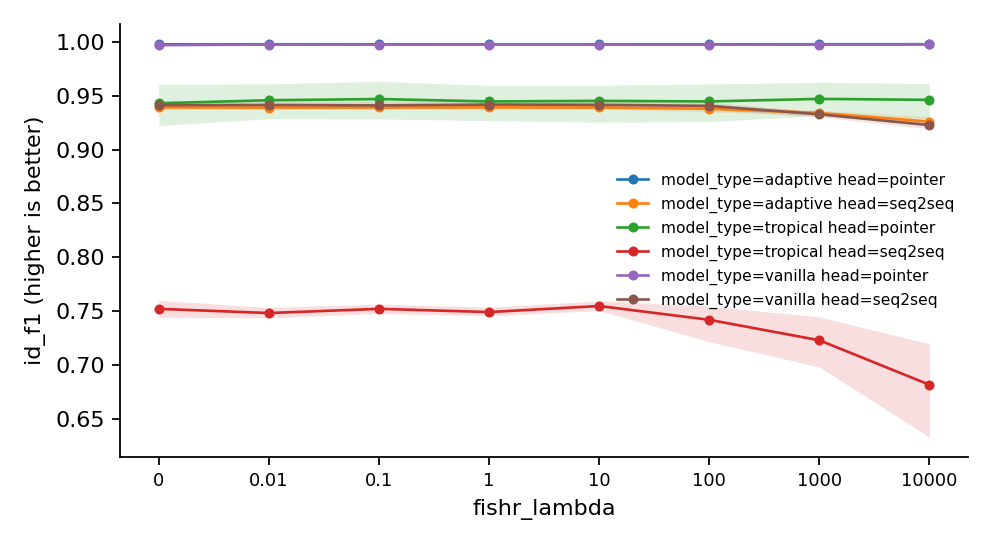
\includegraphics[width=\textwidth]{metric_id_f1.png}
\caption{\texttt{id\_f1} against \texttt{fishr\_lambda}: the mean over seeds with a 95\% bootstrap CI, one line per combination of the other factors.}
\label{fig:id_f1}
\end{figure}

{\small
\begin{longtable}{lllrlrrr}
\caption{\texttt{id\_f1} per cell: mean, 95\% bootstrap CI, SD, seeds, diverged runs.}\label{tab:summary-id_f1}\\
\toprule
\texttt{model\_type} & \texttt{head} & \texttt{fishr\_lambda} & mean & 95\% CI & SD & $n$ & div.\\
\midrule
\endhead
adaptive & pointer & 0 & 0.9976 & [0.997, 0.998] & $7.82\times10^{-4}$ & 5 & 0\\
adaptive & pointer & 0.01 & 0.9977 & [0.997, 0.998] & $2.46\times10^{-4}$ & 5 & 0\\
adaptive & pointer & 0.1 & 0.9976 & [0.997, 0.998] & $3.20\times10^{-4}$ & 5 & 0\\
adaptive & pointer & 1 & 0.9975 & [0.997, 0.998] & $2.93\times10^{-4}$ & 5 & 0\\
adaptive & pointer & 10 & 0.9975 & [0.997, 0.998] & $3.63\times10^{-4}$ & 5 & 0\\
adaptive & pointer & 100 & 0.9976 & [0.997, 0.998] & $3.92\times10^{-4}$ & 5 & 0\\
adaptive & pointer & 1000 & 0.9977 & [0.997, 0.998] & $3.74\times10^{-4}$ & 5 & 0\\
adaptive & pointer & 1e+04 & 0.9977 & [0.998, 0.998] & $1.58\times10^{-4}$ & 5 & 0\\
adaptive & seq2seq & 0 & 0.9391 & [0.938, 0.941] & 0.00206 & 5 & 0\\
adaptive & seq2seq & 0.01 & 0.9389 & [0.937, 0.941] & 0.00246 & 5 & 0\\
adaptive & seq2seq & 0.1 & 0.939 & [0.938, 0.94] & 0.00188 & 5 & 0\\
adaptive & seq2seq & 1 & 0.9391 & [0.937, 0.941] & 0.00247 & 5 & 0\\
adaptive & seq2seq & 10 & 0.939 & [0.937, 0.941] & 0.00219 & 5 & 0\\
adaptive & seq2seq & 100 & 0.9379 & [0.935, 0.941] & 0.00382 & 5 & 0\\
adaptive & seq2seq & 1000 & 0.934 & [0.932, 0.936] & 0.0029 & 5 & 0\\
adaptive & seq2seq & 1e+04 & 0.9259 & [0.922, 0.931] & 0.00557 & 5 & 0\\
tropical & pointer & 0 & 0.943 & [0.922, 0.96] & 0.0252 & 5 & 0\\
tropical & pointer & 0.01 & 0.9458 & [0.929, 0.961] & 0.0218 & 5 & 0\\
tropical & pointer & 0.1 & 0.9469 & [0.928, 0.963] & 0.0232 & 5 & 0\\
tropical & pointer & 1 & 0.9446 & [0.927, 0.96] & 0.0211 & 5 & 0\\
tropical & pointer & 10 & 0.9452 & [0.925, 0.96] & 0.0212 & 5 & 0\\
tropical & pointer & 100 & 0.9446 & [0.926, 0.961] & 0.023 & 5 & 0\\
tropical & pointer & 1000 & 0.947 & [0.932, 0.962] & 0.0203 & 5 & 0\\
tropical & pointer & 1e+04 & 0.9461 & [0.929, 0.961] & 0.022 & 5 & 0\\
tropical & seq2seq & 0 & 0.7523 & [0.744, 0.76] & 0.0103 & 5 & 0\\
tropical & seq2seq & 0.01 & 0.7484 & [0.744, 0.754] & 0.00611 & 5 & 0\\
tropical & seq2seq & 0.1 & 0.7523 & [0.748, 0.757] & 0.00566 & 5 & 0\\
tropical & seq2seq & 1 & 0.7493 & [0.746, 0.754] & 0.00536 & 5 & 0\\
tropical & seq2seq & 10 & 0.7549 & [0.751, 0.76] & 0.00594 & 5 & 0\\
tropical & seq2seq & 100 & 0.7421 & [0.722, 0.755] & 0.023 & 5 & 0\\
tropical & seq2seq & 1000 & 0.7231 & [0.698, 0.745] & 0.0298 & 5 & 0\\
tropical & seq2seq & 1e+04 & 0.6818 & [0.633, 0.72] & 0.0556 & 5 & 0\\
vanilla & pointer & 0 & 0.9969 & [0.997, 0.997] & $2.02\times10^{-4}$ & 5 & 0\\
vanilla & pointer & 0.01 & 0.9974 & [0.997, 0.998] & $3.76\times10^{-4}$ & 5 & 0\\
vanilla & pointer & 0.1 & 0.9974 & [0.997, 0.998] & $3.11\times10^{-4}$ & 5 & 0\\
vanilla & pointer & 1 & 0.9974 & [0.997, 0.998] & $2.53\times10^{-4}$ & 5 & 0\\
vanilla & pointer & 10 & 0.9974 & [0.997, 0.998] & $3.31\times10^{-4}$ & 5 & 0\\
vanilla & pointer & 100 & 0.9973 & [0.997, 0.998] & $4.28\times10^{-4}$ & 5 & 0\\
vanilla & pointer & 1000 & 0.9974 & [0.997, 0.998] & $4.58\times10^{-4}$ & 5 & 0\\
vanilla & pointer & 1e+04 & 0.9976 & [0.997, 0.998] & $2.98\times10^{-4}$ & 5 & 0\\
vanilla & seq2seq & 0 & 0.9412 & [0.939, 0.944] & 0.00353 & 5 & 0\\
vanilla & seq2seq & 0.01 & 0.9414 & [0.939, 0.945] & 0.00411 & 5 & 0\\
vanilla & seq2seq & 0.1 & 0.9409 & [0.938, 0.945] & 0.00445 & 5 & 0\\
vanilla & seq2seq & 1 & 0.9417 & [0.939, 0.946] & 0.00463 & 5 & 0\\
vanilla & seq2seq & 10 & 0.9415 & [0.938, 0.945] & 0.00441 & 5 & 0\\
vanilla & seq2seq & 100 & 0.9405 & [0.937, 0.944] & 0.00446 & 5 & 0\\
vanilla & seq2seq & 1000 & 0.9327 & [0.93, 0.935] & 0.00302 & 5 & 0\\
vanilla & seq2seq & 1e+04 & 0.9227 & [0.919, 0.926] & 0.00493 & 5 & 0\\
\bottomrule
\end{longtable}
}

{\small
\begin{longtable}{lllrrrl}
\caption{\texttt{id\_f1}: each level of \texttt{fishr\_lambda} against its control (0), within each combination of the other factors. rank: Wilcoxon signed-rank by seed, Holm.}\label{tab:control-id_f1}\\
\toprule
\texttt{model\_type} & \texttt{head} & \texttt{fishr\_lambda} & difference & 95\% CI & $p$ & \\
\midrule
\endhead
adaptive & pointer & 0.01 & $1.633\times10^{-4}$ & [$-6.27\times10^{-4}$, $8.00\times10^{-4}$] & 1.0000 & \\
adaptive & pointer & 0.1 & $-1.302\times10^{-4}$ & [$-7.05\times10^{-4}$, $8.06\times10^{-4}$] & 1.0000 & \\
adaptive & pointer & 1 & $-1.952\times10^{-4}$ & [$-7.38\times10^{-4}$, $6.63\times10^{-4}$] & 1.0000 & \\
adaptive & pointer & 10 & $6.044\times10^{-7}$ & [$-8.54\times10^{-4}$, $7.28\times10^{-4}$] & 1.0000 & \\
adaptive & pointer & 100 & 0 & [$-8.53\times10^{-4}$, $7.48\times10^{-4}$] & 1.0000 & \\
adaptive & pointer & 1000 & $3.261\times10^{-4}$ & [$-6.91\times10^{-4}$, $7.41\times10^{-4}$] & 1.0000 & \\
adaptive & pointer & 1e+04 & $1.628\times10^{-4}$ & [$-5.36\times10^{-4}$, $7.80\times10^{-4}$] & 1.0000 & \\
adaptive & seq2seq & 0.01 & $-1.046\times10^{-4}$ & [$-7.10\times10^{-4}$, $2.04\times10^{-4}$] & 1.0000 & \\
adaptive & seq2seq & 0.1 & $1.939\times10^{-5}$ & [$-5.76\times10^{-4}$, $5.85\times10^{-4}$] & 1.0000 & \\
adaptive & seq2seq & 1 & $3.703\times10^{-4}$ & [$-4.62\times10^{-4}$, $3.94\times10^{-4}$] & 1.0000 & \\
adaptive & seq2seq & 10 & $1.464\times10^{-4}$ & [$-6.97\times10^{-4}$, $4.93\times10^{-4}$] & 1.0000 & \\
adaptive & seq2seq & 100 & $-5.759\times10^{-4}$ & [-0.0031, $4.83\times10^{-4}$] & 1.0000 & \\
adaptive & seq2seq & 1000 & -0.005027 & [-0.0062, -0.00399] & 0.4375 & \\
adaptive & seq2seq & 1e+04 & -0.01462 & [-0.0165, -0.00929] & 0.4375 & \\
tropical & pointer & 0.01 & 0.002587 & [$-1.18\times10^{-4}$, 0.00617] & 1.0000 & \\
tropical & pointer & 0.1 & 0.003549 & [0.00105, 0.00672] & 0.8750 & \\
tropical & pointer & 1 & $5.463\times10^{-4}$ & [-0.00131, 0.00529] & 1.0000 & \\
tropical & pointer & 10 & 0.002045 & [$-9.51\times10^{-4}$, 0.00564] & 1.0000 & \\
tropical & pointer & 100 & 0.001366 & [$-2.06\times10^{-4}$, 0.00359] & 1.0000 & \\
tropical & pointer & 1000 & 0.002481 & [$-1.98\times10^{-5}$, 0.00877] & 1.0000 & \\
tropical & pointer & 1e+04 & 0.004979 & [-0.00243, 0.00735] & 1.0000 & \\
tropical & seq2seq & 0.01 & -0.004348 & [-0.00747, $-1.51\times10^{-4}$] & 0.9375 & \\
tropical & seq2seq & 0.1 & $1.289\times10^{-4}$ & [-0.00701, 0.00703] & 1.0000 & \\
tropical & seq2seq & 1 & $-4.252\times10^{-4}$ & [-0.00756, 0.00139] & 1.0000 & \\
tropical & seq2seq & 10 & 0.007708 & [-0.00605, 0.0113] & 1.0000 & \\
tropical & seq2seq & 100 & -0.005418 & [-0.0286, 0.0029] & 1.0000 & \\
tropical & seq2seq & 1000 & -0.02253 & [-0.0502, -0.0114] & 0.4375 & \\
tropical & seq2seq & 1e+04 & -0.04 & [-0.113, -0.0379] & 0.4375 & \\
vanilla & pointer & 0.01 & $5.484\times10^{-4}$ & [$1.88\times10^{-4}$, $8.25\times10^{-4}$] & 0.4375 & \\
vanilla & pointer & 0.1 & $7.168\times10^{-4}$ & [$2.20\times10^{-4}$, $7.98\times10^{-4}$] & 0.4375 & \\
vanilla & pointer & 1 & $5.807\times10^{-4}$ & [$2.93\times10^{-4}$, $7.27\times10^{-4}$] & 0.4375 & \\
vanilla & pointer & 10 & $7.818\times10^{-4}$ & [$2.35\times10^{-4}$, $8.80\times10^{-4}$] & 0.4375 & \\
vanilla & pointer & 100 & $4.185\times10^{-4}$ & [$7.02\times10^{-5}$, $7.86\times10^{-4}$] & 0.4375 & \\
vanilla & pointer & 1000 & $6.451\times10^{-4}$ & [$5.73\times10^{-5}$, $8.96\times10^{-4}$] & 0.4375 & \\
vanilla & pointer & 1e+04 & $9.084\times10^{-4}$ & [$3.25\times10^{-4}$, $9.99\times10^{-4}$] & 0.4375 & \\
vanilla & seq2seq & 0.01 & $1.891\times10^{-4}$ & [$-6.33\times10^{-4}$, $8.13\times10^{-4}$] & 1.0000 & \\
vanilla & seq2seq & 0.1 & $-3.166\times10^{-4}$ & [-0.00102, $5.12\times10^{-4}$] & 1.0000 & \\
vanilla & seq2seq & 1 & $8.694\times10^{-4}$ & [$-5.09\times10^{-4}$, 0.0016] & 1.0000 & \\
vanilla & seq2seq & 10 & $7.210\times10^{-4}$ & [$-6.74\times10^{-4}$, 0.00117] & 1.0000 & \\
vanilla & seq2seq & 100 & $-8.893\times10^{-4}$ & [-0.00171, $7.02\times10^{-4}$] & 1.0000 & \\
vanilla & seq2seq & 1000 & -0.007102 & [-0.0101, -0.00698] & 0.4375 & \\
vanilla & seq2seq & 1e+04 & -0.01801 & [-0.0208, -0.0159] & 0.4375 & \\
\bottomrule
\end{longtable}
}

{\small
\begin{longtable}{llrrrrr}
\caption{\texttt{id\_f1} against log10 \texttt{fishr\_lambda}: rank: Spearman rho, seed-bootstrap CI, with the Jonckheere--Terpstra ordered-trend $\tau$ and $p$.}\label{tab:trend-id_f1}\\
\toprule
\texttt{model\_type} & \texttt{head} & estimate & 95\% CI & $p$ & JT $\tau$ & JT $p$\\
\midrule
\endhead
adaptive & pointer & 0.09625 & [-0.158, 0.281] & 0.5823 & 0.059 & 0.6693\\
adaptive & seq2seq & -0.628 & [-0.825, -0.503] & $<10^{-4}$ & -0.497 & 0.0002\\
tropical & pointer & 0.004243 & [-0.221, 0.217] & 0.9807 & 0.00952 & 0.9512\\
tropical & seq2seq & -0.5106 & [-0.634, -0.33] & 0.0017 & -0.383 & 0.0042\\
vanilla & pointer & 0.06932 & [-0.103, 0.325] & 0.6923 & 0.0514 & 0.7095\\
vanilla & seq2seq & -0.6592 & [-0.77, -0.529] & $<10^{-4}$ & -0.543 & 0.0002\\
\bottomrule
\end{longtable}
}

{\small
\begin{longtable}{lrrrl}
\caption{\texttt{id\_f1}: paired contrasts by seed, Holm-corrected across the cells. rank: Wilcoxon signed-rank by seed, Holm.}\label{tab:paired-id_f1}\\
\toprule
contrast (within) & difference & 95\% CI & $p$ & \\
\midrule
\endhead
\stackcell{model\_type: tropical - vanilla\\\footnotesize head=pointer fishr\_lambda=0 } & -0.05389 & [-0.0851, -0.0227] & 1.0000 & \\
\stackcell{model\_type: tropical - vanilla\\\footnotesize head=pointer fishr\_lambda=0.01 } & -0.05162 & [-0.079, -0.0243] & 1.0000 & \\
\stackcell{model\_type: tropical - vanilla\\\footnotesize head=pointer fishr\_lambda=0.1 } & -0.05052 & [-0.0796, -0.0215] & 1.0000 & \\
\stackcell{model\_type: tropical - vanilla\\\footnotesize head=pointer fishr\_lambda=1 } & -0.05275 & [-0.0791, -0.0264] & 1.0000 & \\
\stackcell{model\_type: tropical - vanilla\\\footnotesize head=pointer fishr\_lambda=10 } & -0.05224 & [-0.0789, -0.0256] & 1.0000 & \\
\stackcell{model\_type: tropical - vanilla\\\footnotesize head=pointer fishr\_lambda=100 } & -0.05266 & [-0.0815, -0.0238] & 1.0000 & \\
\stackcell{model\_type: tropical - vanilla\\\footnotesize head=pointer fishr\_lambda=1000 } & -0.05035 & [-0.0759, -0.0248] & 1.0000 & \\
\stackcell{model\_type: tropical - vanilla\\\footnotesize head=pointer fishr\_lambda=1e+04 } & -0.05146 & [-0.079, -0.0239] & 1.0000 & \\
\stackcell{model\_type: tropical - vanilla\\\footnotesize head=seq2seq fishr\_lambda=0 } & -0.1889 & [-0.203, -0.175] & 1.0000 & \\
\stackcell{model\_type: tropical - vanilla\\\footnotesize head=seq2seq fishr\_lambda=0.01 } & -0.193 & [-0.202, -0.184] & 1.0000 & \\
\stackcell{model\_type: tropical - vanilla\\\footnotesize head=seq2seq fishr\_lambda=0.1 } & -0.1887 & [-0.197, -0.18] & 1.0000 & \\
\stackcell{model\_type: tropical - vanilla\\\footnotesize head=seq2seq fishr\_lambda=1 } & -0.1925 & [-0.201, -0.184] & 1.0000 & \\
\stackcell{model\_type: tropical - vanilla\\\footnotesize head=seq2seq fishr\_lambda=10 } & -0.1866 & [-0.197, -0.176] & 1.0000 & \\
\stackcell{model\_type: tropical - vanilla\\\footnotesize head=seq2seq fishr\_lambda=100 } & -0.1984 & [-0.226, -0.171] & 1.0000 & \\
\stackcell{model\_type: tropical - vanilla\\\footnotesize head=seq2seq fishr\_lambda=1000 } & -0.2096 & [-0.245, -0.174] & 1.0000 & \\
\stackcell{model\_type: tropical - vanilla\\\footnotesize head=seq2seq fishr\_lambda=1e+04 } & -0.2409 & [-0.311, -0.17] & 1.0000 & \\
\stackcell{model\_type: adaptive - vanilla\\\footnotesize head=pointer fishr\_lambda=0 } & $7.129\times10^{-4}$ & [$-4.11\times10^{-4}$, 0.00184] & 1.0000 & \\
\stackcell{model\_type: adaptive - vanilla\\\footnotesize head=pointer fishr\_lambda=0.01 } & $3.055\times10^{-4}$ & [$7.20\times10^{-5}$, $5.39\times10^{-4}$] & 1.0000 & \\
\stackcell{model\_type: adaptive - vanilla\\\footnotesize head=pointer fishr\_lambda=0.1 } & $2.406\times10^{-4}$ & [$-1.33\times10^{-4}$, $6.14\times10^{-4}$] & 1.0000 & \\
\stackcell{model\_type: adaptive - vanilla\\\footnotesize head=pointer fishr\_lambda=1 } & $1.358\times10^{-4}$ & [$-3.69\times10^{-5}$, $3.09\times10^{-4}$] & 1.0000 & \\
\stackcell{model\_type: adaptive - vanilla\\\footnotesize head=pointer fishr\_lambda=10 } & $1.173\times10^{-4}$ & [$-3.68\times10^{-4}$, $6.02\times10^{-4}$] & 1.0000 & \\
\stackcell{model\_type: adaptive - vanilla\\\footnotesize head=pointer fishr\_lambda=100 } & $2.799\times10^{-4}$ & [$-6.96\times10^{-5}$, $6.29\times10^{-4}$] & 1.0000 & \\
\stackcell{model\_type: adaptive - vanilla\\\footnotesize head=pointer fishr\_lambda=1000 } & $3.193\times10^{-4}$ & [$-3.27\times10^{-5}$, $6.71\times10^{-4}$] & 1.0000 & \\
\stackcell{model\_type: adaptive - vanilla\\\footnotesize head=pointer fishr\_lambda=1e+04 } & $1.633\times10^{-4}$ & [$-2.36\times10^{-4}$, $5.62\times10^{-4}$] & 1.0000 & \\
\stackcell{model\_type: adaptive - vanilla\\\footnotesize head=seq2seq fishr\_lambda=0 } & -0.002075 & [-0.00458, $4.34\times10^{-4}$] & 1.0000 & \\
\stackcell{model\_type: adaptive - vanilla\\\footnotesize head=seq2seq fishr\_lambda=0.01 } & -0.002434 & [-0.00525, $3.78\times10^{-4}$] & 1.0000 & \\
\stackcell{model\_type: adaptive - vanilla\\\footnotesize head=seq2seq fishr\_lambda=0.1 } & -0.00191 & [-0.00581, 0.00199] & 1.0000 & \\
\stackcell{model\_type: adaptive - vanilla\\\footnotesize head=seq2seq fishr\_lambda=1 } & -0.002617 & [-0.00626, 0.00103] & 1.0000 & \\
\stackcell{model\_type: adaptive - vanilla\\\footnotesize head=seq2seq fishr\_lambda=10 } & -0.002489 & [-0.00552, $5.44\times10^{-4}$] & 1.0000 & \\
\stackcell{model\_type: adaptive - vanilla\\\footnotesize head=seq2seq fishr\_lambda=100 } & -0.002659 & [-0.00465, $-6.66\times10^{-4}$] & 1.0000 & \\
\stackcell{model\_type: adaptive - vanilla\\\footnotesize head=seq2seq fishr\_lambda=1000 } & 0.001263 & [-0.00115, 0.00368] & 1.0000 & \\
\stackcell{model\_type: adaptive - vanilla\\\footnotesize head=seq2seq fishr\_lambda=1e+04 } & 0.003208 & [$4.90\times10^{-4}$, 0.00593] & 1.0000 & \\
\stackcell{head: pointer - seq2seq\\\footnotesize model\_type=adaptive fishr\_lambda=0 } & 0.05848 & [0.0553, 0.0616] & 1.0000 & \\
\stackcell{head: pointer - seq2seq\\\footnotesize model\_type=adaptive fishr\_lambda=0.01 } & 0.05876 & [0.0555, 0.062] & 1.0000 & \\
\stackcell{head: pointer - seq2seq\\\footnotesize model\_type=adaptive fishr\_lambda=0.1 } & 0.0586 & [0.0561, 0.0611] & 1.0000 & \\
\stackcell{head: pointer - seq2seq\\\footnotesize model\_type=adaptive fishr\_lambda=1 } & 0.0584 & [0.0552, 0.0616] & 1.0000 & \\
\stackcell{head: pointer - seq2seq\\\footnotesize model\_type=adaptive fishr\_lambda=10 } & 0.05851 & [0.0558, 0.0613] & 1.0000 & \\
\stackcell{head: pointer - seq2seq\\\footnotesize model\_type=adaptive fishr\_lambda=100 } & 0.05972 & [0.0549, 0.0645] & 1.0000 & \\
\stackcell{head: pointer - seq2seq\\\footnotesize model\_type=adaptive fishr\_lambda=1000 } & 0.0637 & [0.0599, 0.0675] & 1.0000 & \\
\stackcell{head: pointer - seq2seq\\\footnotesize model\_type=adaptive fishr\_lambda=1e+04 } & 0.07181 & [0.0649, 0.0787] & 1.0000 & \\
\stackcell{head: pointer - seq2seq\\\footnotesize model\_type=tropical fishr\_lambda=0 } & 0.1907 & [0.159, 0.223] & 1.0000 & \\
\stackcell{head: pointer - seq2seq\\\footnotesize model\_type=tropical fishr\_lambda=0.01 } & 0.1974 & [0.171, 0.224] & 1.0000 & \\
\stackcell{head: pointer - seq2seq\\\footnotesize model\_type=tropical fishr\_lambda=0.1 } & 0.1946 & [0.17, 0.22] & 1.0000 & \\
\stackcell{head: pointer - seq2seq\\\footnotesize model\_type=tropical fishr\_lambda=1 } & 0.1954 & [0.17, 0.221] & 1.0000 & \\
\stackcell{head: pointer - seq2seq\\\footnotesize model\_type=tropical fishr\_lambda=10 } & 0.1903 & [0.162, 0.218] & 1.0000 & \\
\stackcell{head: pointer - seq2seq\\\footnotesize model\_type=tropical fishr\_lambda=100 } & 0.2025 & [0.163, 0.242] & 1.0000 & \\
\stackcell{head: pointer - seq2seq\\\footnotesize model\_type=tropical fishr\_lambda=1000 } & 0.2239 & [0.174, 0.274] & 1.0000 & \\
\stackcell{head: pointer - seq2seq\\\footnotesize model\_type=tropical fishr\_lambda=1e+04 } & 0.2643 & [0.182, 0.346] & 1.0000 & \\
\stackcell{head: pointer - seq2seq\\\footnotesize model\_type=vanilla fishr\_lambda=0 } & 0.05569 & [0.0514, 0.06] & 1.0000 & \\
\stackcell{head: pointer - seq2seq\\\footnotesize model\_type=vanilla fishr\_lambda=0.01 } & 0.05602 & [0.0506, 0.0614] & 1.0000 & \\
\stackcell{head: pointer - seq2seq\\\footnotesize model\_type=vanilla fishr\_lambda=0.1 } & 0.05645 & [0.0506, 0.0623] & 1.0000 & \\
\stackcell{head: pointer - seq2seq\\\footnotesize model\_type=vanilla fishr\_lambda=1 } & 0.05565 & [0.0497, 0.0615] & 1.0000 & \\
\stackcell{head: pointer - seq2seq\\\footnotesize model\_type=vanilla fishr\_lambda=10 } & 0.0559 & [0.05, 0.0618] & 1.0000 & \\
\stackcell{head: pointer - seq2seq\\\footnotesize model\_type=vanilla fishr\_lambda=100 } & 0.05678 & [0.0509, 0.0627] & 1.0000 & \\
\stackcell{head: pointer - seq2seq\\\footnotesize model\_type=vanilla fishr\_lambda=1000 } & 0.06464 & [0.0606, 0.0687] & 1.0000 & \\
\stackcell{head: pointer - seq2seq\\\footnotesize model\_type=vanilla fishr\_lambda=1e+04 } & 0.07486 & [0.0684, 0.0813] & 1.0000 & \\
\bottomrule
\end{longtable}
}

\subsection{\texttt{id\_exact}}
\begin{figure}[tbp]
\centering
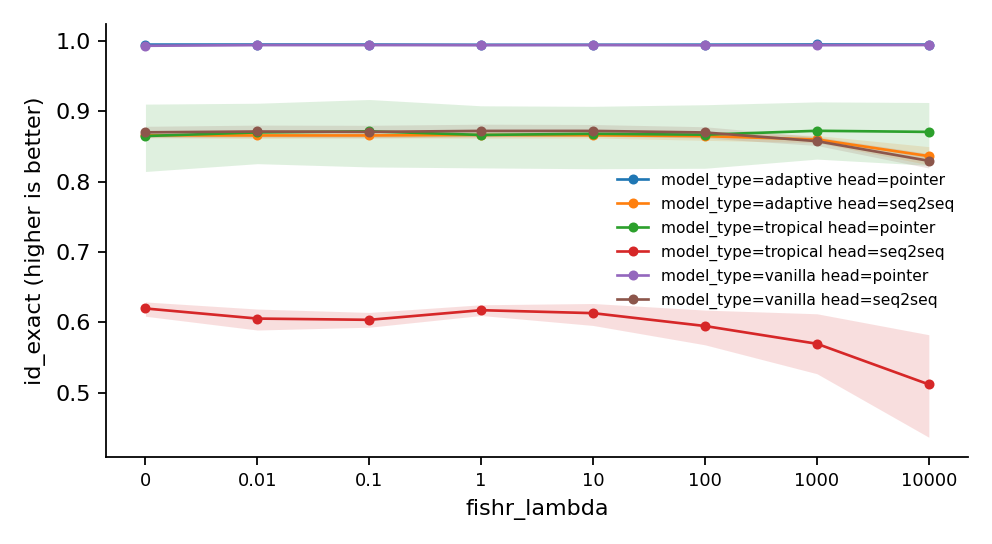
\includegraphics[width=\textwidth]{metric_id_exact.png}
\caption{\texttt{id\_exact} against \texttt{fishr\_lambda}: the mean over seeds with a 95\% bootstrap CI, one line per combination of the other factors.}
\label{fig:id_exact}
\end{figure}

{\small
\begin{longtable}{lllrlrrr}
\caption{\texttt{id\_exact} per cell: mean, 95\% bootstrap CI, SD, seeds, diverged runs.}\label{tab:summary-id_exact}\\
\toprule
\texttt{model\_type} & \texttt{head} & \texttt{fishr\_lambda} & mean & 95\% CI & SD & $n$ & div.\\
\midrule
\endhead
adaptive & pointer & 0 & 0.9949 & [0.993, 0.996] & 0.00161 & 5 & 0\\
adaptive & pointer & 0.01 & 0.9949 & [0.994, 0.995] & $6.88\times10^{-4}$ & 5 & 0\\
adaptive & pointer & 0.1 & 0.9949 & [0.994, 0.995] & $6.75\times10^{-4}$ & 5 & 0\\
adaptive & pointer & 1 & 0.9946 & [0.994, 0.995] & $6.20\times10^{-4}$ & 5 & 0\\
adaptive & pointer & 10 & 0.9946 & [0.994, 0.995] & $8.35\times10^{-4}$ & 5 & 0\\
adaptive & pointer & 100 & 0.9948 & [0.994, 0.995] & $8.70\times10^{-4}$ & 5 & 0\\
adaptive & pointer & 1000 & 0.995 & [0.994, 0.996] & $8.93\times10^{-4}$ & 5 & 0\\
adaptive & pointer & 1e+04 & 0.9949 & [0.995, 0.995] & $4.92\times10^{-4}$ & 5 & 0\\
adaptive & seq2seq & 0 & 0.8658 & [0.862, 0.869] & 0.00458 & 5 & 0\\
adaptive & seq2seq & 0.01 & 0.8657 & [0.861, 0.87] & 0.00565 & 5 & 0\\
adaptive & seq2seq & 0.1 & 0.8657 & [0.862, 0.869] & 0.00492 & 5 & 0\\
adaptive & seq2seq & 1 & 0.8663 & [0.862, 0.871] & 0.00603 & 5 & 0\\
adaptive & seq2seq & 10 & 0.8659 & [0.862, 0.87] & 0.00526 & 5 & 0\\
adaptive & seq2seq & 100 & 0.8647 & [0.859, 0.871] & 0.00797 & 5 & 0\\
adaptive & seq2seq & 1000 & 0.86 & [0.855, 0.866] & 0.00651 & 5 & 0\\
adaptive & seq2seq & 1e+04 & 0.8362 & [0.824, 0.85] & 0.016 & 5 & 0\\
tropical & pointer & 0 & 0.8648 & [0.814, 0.91] & 0.0644 & 5 & 0\\
tropical & pointer & 0.01 & 0.87 & [0.826, 0.911] & 0.0576 & 5 & 0\\
tropical & pointer & 0.1 & 0.8715 & [0.821, 0.917] & 0.063 & 5 & 0\\
tropical & pointer & 1 & 0.8664 & [0.82, 0.908] & 0.0557 & 5 & 0\\
tropical & pointer & 10 & 0.8681 & [0.818, 0.907] & 0.0559 & 5 & 0\\
tropical & pointer & 100 & 0.8667 & [0.819, 0.909] & 0.0603 & 5 & 0\\
tropical & pointer & 1000 & 0.8723 & [0.832, 0.913] & 0.0548 & 5 & 0\\
tropical & pointer & 1e+04 & 0.8707 & [0.823, 0.913] & 0.0591 & 5 & 0\\
tropical & seq2seq & 0 & 0.6196 & [0.609, 0.629] & 0.0133 & 5 & 0\\
tropical & seq2seq & 0.01 & 0.6052 & [0.589, 0.619] & 0.0194 & 5 & 0\\
tropical & seq2seq & 0.1 & 0.6035 & [0.593, 0.614] & 0.0144 & 5 & 0\\
tropical & seq2seq & 1 & 0.6172 & [0.61, 0.625] & 0.01 & 5 & 0\\
tropical & seq2seq & 10 & 0.613 & [0.595, 0.627] & 0.0201 & 5 & 0\\
tropical & seq2seq & 100 & 0.5947 & [0.568, 0.617] & 0.0309 & 5 & 0\\
tropical & seq2seq & 1000 & 0.5694 & [0.527, 0.612] & 0.0558 & 5 & 0\\
tropical & seq2seq & 1e+04 & 0.5116 & [0.436, 0.582] & 0.0964 & 5 & 0\\
vanilla & pointer & 0 & 0.9932 & [0.993, 0.994] & $5.10\times10^{-4}$ & 5 & 0\\
vanilla & pointer & 0.01 & 0.9942 & [0.994, 0.995] & $8.38\times10^{-4}$ & 5 & 0\\
vanilla & pointer & 0.1 & 0.9942 & [0.994, 0.995] & $9.07\times10^{-4}$ & 5 & 0\\
vanilla & pointer & 1 & 0.9941 & [0.994, 0.995] & $6.76\times10^{-4}$ & 5 & 0\\
vanilla & pointer & 10 & 0.9942 & [0.994, 0.995] & $6.27\times10^{-4}$ & 5 & 0\\
vanilla & pointer & 100 & 0.9939 & [0.993, 0.995] & $9.35\times10^{-4}$ & 5 & 0\\
vanilla & pointer & 1000 & 0.994 & [0.993, 0.995] & 0.00107 & 5 & 0\\
vanilla & pointer & 1e+04 & 0.9943 & [0.994, 0.995] & $5.70\times10^{-4}$ & 5 & 0\\
vanilla & seq2seq & 0 & 0.8701 & [0.863, 0.879] & 0.0101 & 5 & 0\\
vanilla & seq2seq & 0.01 & 0.8713 & [0.863, 0.88] & 0.0109 & 5 & 0\\
vanilla & seq2seq & 0.1 & 0.8708 & [0.862, 0.88] & 0.0116 & 5 & 0\\
vanilla & seq2seq & 1 & 0.8721 & [0.864, 0.882] & 0.0115 & 5 & 0\\
vanilla & seq2seq & 10 & 0.8721 & [0.864, 0.881] & 0.0108 & 5 & 0\\
vanilla & seq2seq & 100 & 0.8699 & [0.862, 0.878] & 0.0104 & 5 & 0\\
vanilla & seq2seq & 1000 & 0.8575 & [0.851, 0.864] & 0.0079 & 5 & 0\\
vanilla & seq2seq & 1e+04 & 0.8296 & [0.819, 0.84] & 0.0136 & 5 & 0\\
\bottomrule
\end{longtable}
}

{\small
\begin{longtable}{lllrrrl}
\caption{\texttt{id\_exact}: each level of \texttt{fishr\_lambda} against its control (0), within each combination of the other factors. rank: Wilcoxon signed-rank by seed, Holm.}\label{tab:control-id_exact}\\
\toprule
\texttt{model\_type} & \texttt{head} & \texttt{fishr\_lambda} & difference & 95\% CI & $p$ & \\
\midrule
\endhead
adaptive & pointer & 0.01 & $1.000\times10^{-4}$ & [-0.00168, 0.0017] & 1.0000 & \\
adaptive & pointer & 0.1 & $-3.000\times10^{-4}$ & [-0.0017, 0.00172] & 1.0000 & \\
adaptive & pointer & 1 & $-6.000\times10^{-4}$ & [-0.00194, 0.0013] & 1.0000 & \\
adaptive & pointer & 10 & $-4.000\times10^{-4}$ & [-0.00216, 0.00146] & 1.0000 & \\
adaptive & pointer & 100 & $-1.000\times10^{-4}$ & [-0.00202, 0.00162] & 1.0000 & \\
adaptive & pointer & 1000 & $4.000\times10^{-4}$ & [-0.00184, 0.00182] & 1.0000 & \\
adaptive & pointer & 1e+04 & $1.000\times10^{-4}$ & [-0.00162, 0.0014] & 1.0000 & \\
adaptive & seq2seq & 0.01 & $-4.000\times10^{-4}$ & [-0.00114, $7.60\times10^{-4}$] & 1.0000 & \\
adaptive & seq2seq & 0.1 & $-5.000\times10^{-4}$ & [-0.00104, $8.40\times10^{-4}$] & 1.0000 & \\
adaptive & seq2seq & 1 & $6.000\times10^{-4}$ & [$-7.20\times10^{-4}$, 0.00168] & 1.0000 & \\
adaptive & seq2seq & 10 & $5.000\times10^{-4}$ & [$-8.80\times10^{-4}$, $9.00\times10^{-4}$] & 1.0000 & \\
adaptive & seq2seq & 100 & $-3.000\times10^{-4}$ & [-0.00442, 0.0019] & 1.0000 & \\
adaptive & seq2seq & 1000 & -0.0066 & [-0.00716, -0.00394] & 0.4375 & \\
adaptive & seq2seq & 1e+04 & -0.0315 & [-0.0385, -0.0193] & 0.4375 & \\
tropical & pointer & 0.01 & 0.0035 & [-0.0019, 0.0125] & 1.0000 & \\
tropical & pointer & 0.1 & 0.0062 & [$9.20\times10^{-4}$, 0.0132] & 0.8750 & \\
tropical & pointer & 1 & 0.0016 & [-0.00504, 0.00872] & 1.0000 & \\
tropical & pointer & 10 & 0.0051 & [-0.00428, 0.00992] & 1.0000 & \\
tropical & pointer & 100 & 0.0043 & [-0.00386, 0.00594] & 1.0000 & \\
tropical & pointer & 1000 & 0.006 & [-0.0013, 0.0176] & 1.0000 & \\
tropical & pointer & 1e+04 & 0.0097 & [-0.00829, 0.017] & 1.0000 & \\
tropical & seq2seq & 0.01 & -0.0098 & [-0.0203, -0.00878] & 0.4375 & \\
tropical & seq2seq & 0.1 & -0.0178 & [-0.0224, -0.0113] & 0.4375 & \\
tropical & seq2seq & 1 & -0.0044 & [-0.0127, 0.0078] & 0.8125 & \\
tropical & seq2seq & 10 & -0.0125 & [-0.015, 0.00362] & 0.6250 & \\
tropical & seq2seq & 100 & -0.0185 & [-0.0495, -0.00614] & 0.4375 & \\
tropical & seq2seq & 1000 & -0.0452 & [-0.0863, -0.0141] & 0.4375 & \\
tropical & seq2seq & 1e+04 & -0.0552 & [-0.172, -0.0448] & 0.4375 & \\
vanilla & pointer & 0.01 & $8.000\times10^{-4}$ & [$3.00\times10^{-4}$, 0.00158] & 0.6250 & \\
vanilla & pointer & 0.1 & 0.0012 & [$1.40\times10^{-4}$, 0.0017] & 0.6250 & \\
vanilla & pointer & 1 & $9.000\times10^{-4}$ & [$4.19\times10^{-4}$, 0.00132] & 0.4375 & \\
vanilla & pointer & 10 & 0.0012 & [$4.20\times10^{-4}$, 0.00158] & 0.6250 & \\
vanilla & pointer & 100 & $6.000\times10^{-4}$ & [$2.00\times10^{-5}$, 0.00136] & 0.6250 & \\
vanilla & pointer & 1000 & $6.000\times10^{-4}$ & [$6.00\times10^{-5}$, 0.0016] & 0.6250 & \\
vanilla & pointer & 1e+04 & 0.0012 & [$6.00\times10^{-4}$, 0.00152] & 0.4375 & \\
vanilla & seq2seq & 0.01 & 0.0019 & [$-6.00\times10^{-5}$, 0.00246] & 0.9375 & \\
vanilla & seq2seq & 0.1 & 0.0018 & [$-8.80\times10^{-4}$, 0.00204] & 1.0000 & \\
vanilla & seq2seq & 1 & 0.0027 & [$5.00\times10^{-4}$, 0.00348] & 0.7500 & \\
vanilla & seq2seq & 10 & 0.0023 & [$8.60\times10^{-4}$, 0.00278] & 0.6250 & \\
vanilla & seq2seq & 100 & 0 & [-0.0018, 0.00152] & 1.0000 & \\
vanilla & seq2seq & 1000 & -0.0115 & [-0.0164, -0.00926] & 0.4375 & \\
vanilla & seq2seq & 1e+04 & -0.0435 & [-0.0464, -0.0333] & 0.4375 & \\
\bottomrule
\end{longtable}
}

{\small
\begin{longtable}{llrrrrr}
\caption{\texttt{id\_exact} against log10 \texttt{fishr\_lambda}: rank: Spearman rho, seed-bootstrap CI, with the Jonckheere--Terpstra ordered-trend $\tau$ and $p$.}\label{tab:trend-id_exact}\\
\toprule
\texttt{model\_type} & \texttt{head} & estimate & 95\% CI & $p$ & JT $\tau$ & JT $p$\\
\midrule
\endhead
adaptive & pointer & 0.03407 & [-0.205, 0.29] & 0.8459 & 0.0324 & 0.8142\\
adaptive & seq2seq & -0.5065 & [-0.776, -0.364] & 0.0019 & -0.41 & 0.0018\\
tropical & pointer & 0.02829 & [-0.221, 0.315] & 0.8718 & 0.0286 & 0.8354\\
tropical & seq2seq & -0.4088 & [-0.652, -0.143] & 0.0148 & -0.295 & 0.0314\\
vanilla & pointer & 0 & [-0.12, 0.146] & 1.0000 & -0.00381 & 0.9834\\
vanilla & seq2seq & -0.5319 & [-0.702, -0.388] & 0.0010 & -0.421 & 0.0016\\
\bottomrule
\end{longtable}
}

{\small
\begin{longtable}{lrrrl}
\caption{\texttt{id\_exact}: paired contrasts by seed, Holm-corrected across the cells. rank: Wilcoxon signed-rank by seed, Holm.}\label{tab:paired-id_exact}\\
\toprule
contrast (within) & difference & 95\% CI & $p$ & \\
\midrule
\endhead
\stackcell{model\_type: tropical - vanilla\\\footnotesize head=pointer fishr\_lambda=0 } & -0.1284 & [-0.208, -0.0484] & 1.0000 & \\
\stackcell{model\_type: tropical - vanilla\\\footnotesize head=pointer fishr\_lambda=0.01 } & -0.1242 & [-0.196, -0.0521] & 1.0000 & \\
\stackcell{model\_type: tropical - vanilla\\\footnotesize head=pointer fishr\_lambda=0.1 } & -0.1226 & [-0.202, -0.0437] & 1.0000 & \\
\stackcell{model\_type: tropical - vanilla\\\footnotesize head=pointer fishr\_lambda=1 } & -0.1277 & [-0.197, -0.0583] & 1.0000 & \\
\stackcell{model\_type: tropical - vanilla\\\footnotesize head=pointer fishr\_lambda=10 } & -0.1262 & [-0.196, -0.0563] & 1.0000 & \\
\stackcell{model\_type: tropical - vanilla\\\footnotesize head=pointer fishr\_lambda=100 } & -0.1272 & [-0.203, -0.0517] & 1.0000 & \\
\stackcell{model\_type: tropical - vanilla\\\footnotesize head=pointer fishr\_lambda=1000 } & -0.1217 & [-0.191, -0.0529] & 1.0000 & \\
\stackcell{model\_type: tropical - vanilla\\\footnotesize head=pointer fishr\_lambda=1e+04 } & -0.1236 & [-0.197, -0.0497] & 1.0000 & \\
\stackcell{model\_type: tropical - vanilla\\\footnotesize head=seq2seq fishr\_lambda=0 } & -0.2505 & [-0.276, -0.225] & 1.0000 & \\
\stackcell{model\_type: tropical - vanilla\\\footnotesize head=seq2seq fishr\_lambda=0.01 } & -0.2661 & [-0.3, -0.232] & 1.0000 & \\
\stackcell{model\_type: tropical - vanilla\\\footnotesize head=seq2seq fishr\_lambda=0.1 } & -0.2673 & [-0.295, -0.24] & 1.0000 & \\
\stackcell{model\_type: tropical - vanilla\\\footnotesize head=seq2seq fishr\_lambda=1 } & -0.255 & [-0.277, -0.232] & 1.0000 & \\
\stackcell{model\_type: tropical - vanilla\\\footnotesize head=seq2seq fishr\_lambda=10 } & -0.2592 & [-0.296, -0.222] & 1.0000 & \\
\stackcell{model\_type: tropical - vanilla\\\footnotesize head=seq2seq fishr\_lambda=100 } & -0.2752 & [-0.315, -0.236] & 1.0000 & \\
\stackcell{model\_type: tropical - vanilla\\\footnotesize head=seq2seq fishr\_lambda=1000 } & -0.2881 & [-0.358, -0.218] & 1.0000 & \\
\stackcell{model\_type: tropical - vanilla\\\footnotesize head=seq2seq fishr\_lambda=1e+04 } & -0.3179 & [-0.441, -0.195] & 1.0000 & \\
\stackcell{model\_type: adaptive - vanilla\\\footnotesize head=pointer fishr\_lambda=0 } & 0.0017 & [$-5.49\times10^{-4}$, 0.00395] & 1.0000 & \\
\stackcell{model\_type: adaptive - vanilla\\\footnotesize head=pointer fishr\_lambda=0.01 } & $7.800\times10^{-4}$ & [$1.88\times10^{-4}$, 0.00137] & 1.0000 & \\
\stackcell{model\_type: adaptive - vanilla\\\footnotesize head=pointer fishr\_lambda=0.1 } & $7.400\times10^{-4}$ & [$-2.86\times10^{-4}$, 0.00177] & 1.0000 & \\
\stackcell{model\_type: adaptive - vanilla\\\footnotesize head=pointer fishr\_lambda=1 } & $5.200\times10^{-4}$ & [$1.87\times10^{-4}$, $8.53\times10^{-4}$] & 1.0000 & \\
\stackcell{model\_type: adaptive - vanilla\\\footnotesize head=pointer fishr\_lambda=10 } & $4.000\times10^{-4}$ & [$-5.78\times10^{-4}$, 0.00138] & 1.0000 & \\
\stackcell{model\_type: adaptive - vanilla\\\footnotesize head=pointer fishr\_lambda=100 } & $8.800\times10^{-4}$ & [$-4.25\times10^{-5}$, 0.0018] & 1.0000 & \\
\stackcell{model\_type: adaptive - vanilla\\\footnotesize head=pointer fishr\_lambda=1000 } & 0.001 & [$2.23\times10^{-5}$, 0.00198] & 1.0000 & \\
\stackcell{model\_type: adaptive - vanilla\\\footnotesize head=pointer fishr\_lambda=1e+04 } & $5.800\times10^{-4}$ & [$1.38\times10^{-4}$, 0.00102] & 1.0000 & \\
\stackcell{model\_type: adaptive - vanilla\\\footnotesize head=seq2seq fishr\_lambda=0 } & -0.00426 & [-0.0129, 0.00437] & 1.0000 & \\
\stackcell{model\_type: adaptive - vanilla\\\footnotesize head=seq2seq fishr\_lambda=0.01 } & -0.00562 & [-0.0142, 0.00292] & 1.0000 & \\
\stackcell{model\_type: adaptive - vanilla\\\footnotesize head=seq2seq fishr\_lambda=0.1 } & -0.0051 & [-0.0156, 0.00545] & 1.0000 & \\
\stackcell{model\_type: adaptive - vanilla\\\footnotesize head=seq2seq fishr\_lambda=1 } & -0.0058 & [-0.0153, 0.00371] & 1.0000 & \\
\stackcell{model\_type: adaptive - vanilla\\\footnotesize head=seq2seq fishr\_lambda=10 } & -0.0062 & [-0.0145, 0.00212] & 1.0000 & \\
\stackcell{model\_type: adaptive - vanilla\\\footnotesize head=seq2seq fishr\_lambda=100 } & -0.00524 & [-0.0109, $4.51\times10^{-4}$] & 1.0000 & \\
\stackcell{model\_type: adaptive - vanilla\\\footnotesize head=seq2seq fishr\_lambda=1000 } & 0.00248 & [-0.00279, 0.00775] & 1.0000 & \\
\stackcell{model\_type: adaptive - vanilla\\\footnotesize head=seq2seq fishr\_lambda=1e+04 } & 0.00666 & [-0.00155, 0.0149] & 1.0000 & \\
\stackcell{head: pointer - seq2seq\\\footnotesize model\_type=adaptive fishr\_lambda=0 } & 0.1291 & [0.122, 0.136] & 1.0000 & \\
\stackcell{head: pointer - seq2seq\\\footnotesize model\_type=adaptive fishr\_lambda=0.01 } & 0.1293 & [0.122, 0.137] & 1.0000 & \\
\stackcell{head: pointer - seq2seq\\\footnotesize model\_type=adaptive fishr\_lambda=0.1 } & 0.1292 & [0.123, 0.136] & 1.0000 & \\
\stackcell{head: pointer - seq2seq\\\footnotesize model\_type=adaptive fishr\_lambda=1 } & 0.1283 & [0.121, 0.136] & 1.0000 & \\
\stackcell{head: pointer - seq2seq\\\footnotesize model\_type=adaptive fishr\_lambda=10 } & 0.1287 & [0.122, 0.135] & 1.0000 & \\
\stackcell{head: pointer - seq2seq\\\footnotesize model\_type=adaptive fishr\_lambda=100 } & 0.1301 & [0.12, 0.14] & 1.0000 & \\
\stackcell{head: pointer - seq2seq\\\footnotesize model\_type=adaptive fishr\_lambda=1000 } & 0.135 & [0.127, 0.143] & 1.0000 & \\
\stackcell{head: pointer - seq2seq\\\footnotesize model\_type=adaptive fishr\_lambda=1e+04 } & 0.1587 & [0.139, 0.178] & 1.0000 & \\
\stackcell{head: pointer - seq2seq\\\footnotesize model\_type=tropical fishr\_lambda=0 } & 0.2452 & [0.156, 0.334] & 1.0000 & \\
\stackcell{head: pointer - seq2seq\\\footnotesize model\_type=tropical fishr\_lambda=0.01 } & 0.2648 & [0.183, 0.346] & 1.0000 & \\
\stackcell{head: pointer - seq2seq\\\footnotesize model\_type=tropical fishr\_lambda=0.1 } & 0.2681 & [0.186, 0.35] & 1.0000 & \\
\stackcell{head: pointer - seq2seq\\\footnotesize model\_type=tropical fishr\_lambda=1 } & 0.2492 & [0.17, 0.328] & 1.0000 & \\
\stackcell{head: pointer - seq2seq\\\footnotesize model\_type=tropical fishr\_lambda=10 } & 0.2551 & [0.173, 0.337] & 1.0000 & \\
\stackcell{head: pointer - seq2seq\\\footnotesize model\_type=tropical fishr\_lambda=100 } & 0.2721 & [0.182, 0.362] & 1.0000 & \\
\stackcell{head: pointer - seq2seq\\\footnotesize model\_type=tropical fishr\_lambda=1000 } & 0.3029 & [0.182, 0.423] & 1.0000 & \\
\stackcell{head: pointer - seq2seq\\\footnotesize model\_type=tropical fishr\_lambda=1e+04 } & 0.3591 & [0.198, 0.52] & 1.0000 & \\
\stackcell{head: pointer - seq2seq\\\footnotesize model\_type=vanilla fishr\_lambda=0 } & 0.1231 & [0.111, 0.136] & 1.0000 & \\
\stackcell{head: pointer - seq2seq\\\footnotesize model\_type=vanilla fishr\_lambda=0.01 } & 0.1229 & [0.109, 0.137] & 1.0000 & \\
\stackcell{head: pointer - seq2seq\\\footnotesize model\_type=vanilla fishr\_lambda=0.1 } & 0.1234 & [0.108, 0.138] & 1.0000 & \\
\stackcell{head: pointer - seq2seq\\\footnotesize model\_type=vanilla fishr\_lambda=1 } & 0.122 & [0.108, 0.136] & 1.0000 & \\
\stackcell{head: pointer - seq2seq\\\footnotesize model\_type=vanilla fishr\_lambda=10 } & 0.1221 & [0.108, 0.136] & 1.0000 & \\
\stackcell{head: pointer - seq2seq\\\footnotesize model\_type=vanilla fishr\_lambda=100 } & 0.124 & [0.11, 0.138] & 1.0000 & \\
\stackcell{head: pointer - seq2seq\\\footnotesize model\_type=vanilla fishr\_lambda=1000 } & 0.1365 & [0.126, 0.147] & 1.0000 & \\
\stackcell{head: pointer - seq2seq\\\footnotesize model\_type=vanilla fishr\_lambda=1e+04 } & 0.1647 & [0.147, 0.182] & 1.0000 & \\
\bottomrule
\end{longtable}
}


\section{Curves}
\begin{figure}[tbp]
\centering
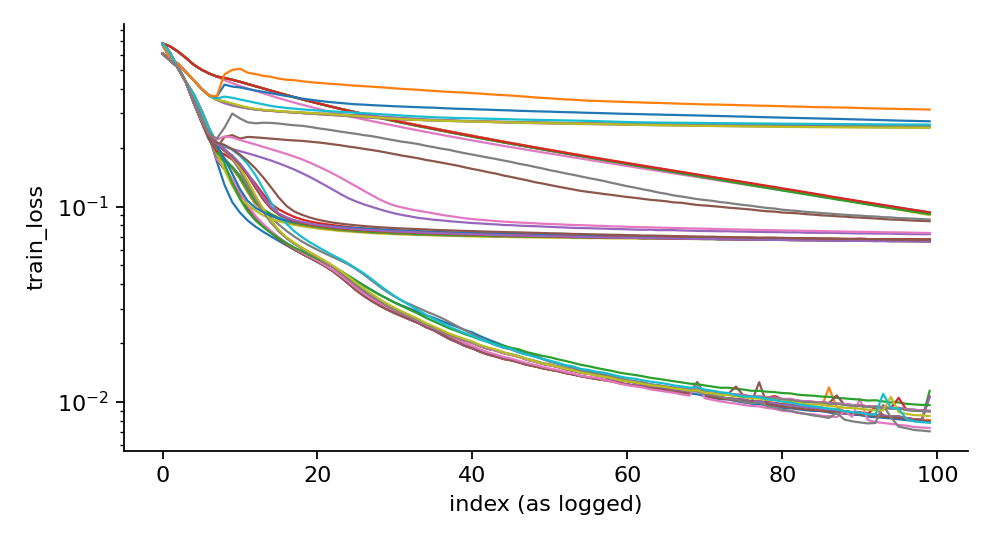
\includegraphics[width=\textwidth]{curve_train_loss.png}
\caption{\texttt{train\_loss}, the mean over seeds per cell.}
\label{fig:curve-1}
\end{figure}
\begin{figure}[tbp]
\centering
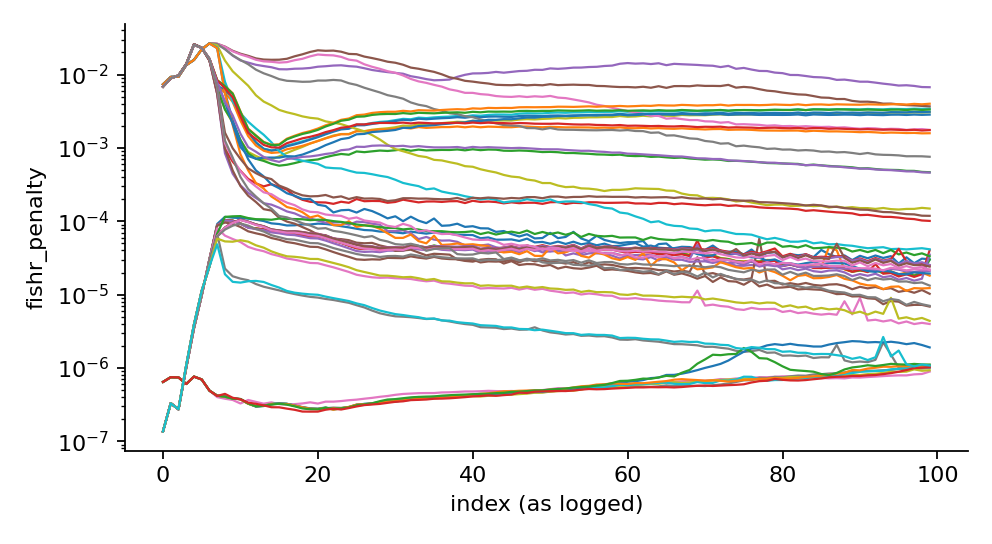
\includegraphics[width=\textwidth]{curve_fishr_penalty.png}
\caption{\texttt{fishr\_penalty}, the mean over seeds per cell.}
\label{fig:curve-2}
\end{figure}
\begin{figure}[tbp]
\centering
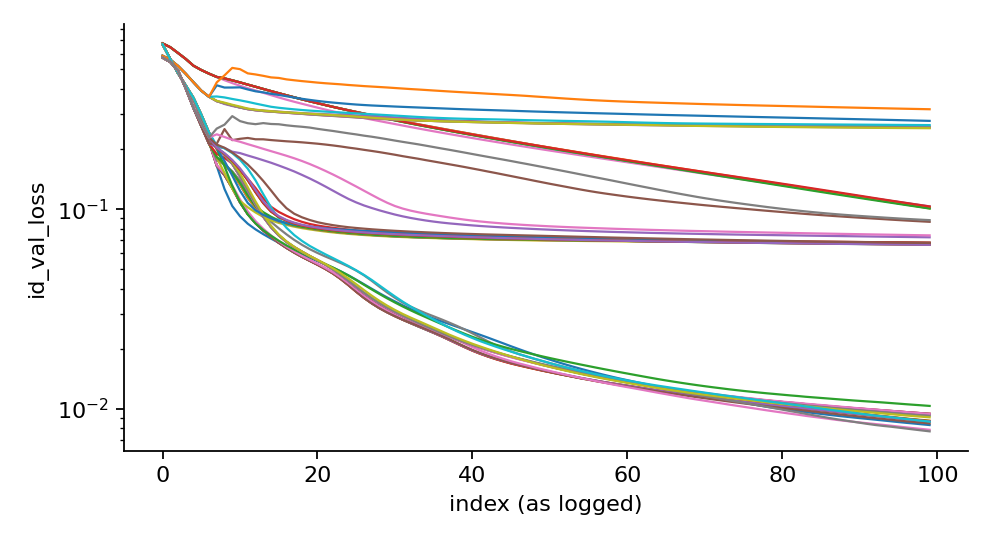
\includegraphics[width=\textwidth]{curve_id_val_loss.png}
\caption{\texttt{id\_val\_loss}, the mean over seeds per cell.}
\label{fig:curve-3}
\end{figure}

\section{Configuration}
The base configuration every run shares (frozen hash \texttt{bd73c304e6b9}); factor levels are in \autoref{tab:summary-ood_len_f1}.
{\footnotesize
\begin{verbatim}
task:
  name: QuickselectDataset
  value_range:
  - 1
  - 10
  target_range: null
  weight_range: null
  adversarial_range:
  - 10
  - 30
  noise_prob: 0.0
data:
  train_lengths:
  - 4
  - 5
  - 6
  - 7
  - 8
  ood_lengths:
  - 12
  - 16
  - 64
  ood_value_range:
  - 11
  - 21
  ood_noise_range:
  - 1
  - 5
  ood_noise_prob: 0.5
  n_per_length: 20000
  n_eval_per_length: 2000
  curve_eval_limit: 256
model:
  d_model: 64
  n_heads: 2
  num_layers: 1
  dropout: 0.0
  tropical_impl: legacy
optim:
  lr: 0.0001
  epochs: 100
  batch_size: 100
  eval_batch_size: 256
fishr:
  ema: 0.95
  anneal_iters: 1500
  reset_optimizer: true
\end{verbatim}
}
Store: \texttt{campaigns/tropical/Quickselect/results}.
\end{document}